\documentclass[12pt, oneside, openany]{report}
%\usepackage{IEEEtrantools}

\usepackage[lmargin=2cm, rmargin=2cm, tmargin=2cm, bmargin=2.5cm, footnotesep=2cm, footskip=1cm]{geometry}
\linespread{1.5}
\usepackage{hyperref}
\usepackage{mathptmx}
\usepackage[table,xcdraw]{xcolor}
\usepackage{lscape}
\usepackage{longtable}
\usepackage{booktabs}
\usepackage{hyperref}
\usepackage[utf8x]{inputenc}
\usepackage[english]{babel}
\usepackage[
    backend=biber,
    style=ieee,
    backref=true,
    isbn=false,
    isbn=false,
    natbib=true,
    defernumbers=true
    ]{biblatex}
\usepackage[section]{placeins}
\usepackage[parfill = 20pt]{parskip}

\DeclareBibliographyCategory{cited}
\AtEveryCitekey{\addtocategory{cited}{\thefield{entrykey}}}
%\usepackage{filecontents}
\addbibresource{references.bib}
\nocite{*}

\AtEveryBibitem{
    \clearfield{urlyear}
    \clearfield{urlmonth}
}
\usepackage{float}
\usepackage{listings}

\definecolor{codegreen}{rgb}{0,0.6,0}
\definecolor{codegray}{rgb}{0.5,0.5,0.5}
\definecolor{codepurple}{rgb}{0.58,0,0.82}
\definecolor{backcolour}{rgb}{0.95,0.95,0.92}

\lstdefinestyle{mystyle}{
    backgroundcolor=\color{backcolour},   
    commentstyle=\color{codegreen},
    keywordstyle=\color{magenta},
    numberstyle=\tiny\color{codegray},
    stringstyle=\color{codepurple},
    basicstyle=\ttfamily\footnotesize,
    breakatwhitespace=false,         
    breaklines=true,                 
    captionpos=b,                    
    keepspaces=true,                 
    numbers=left,                    
    numbersep=5pt,                  
    showspaces=false,                
    showstringspaces=false,
    showtabs=false,                  
    tabsize=2
}

\lstset{style=mystyle}



%\usepackage[style=authoryear, defernumbers=true, backend=biber,dashed=false, maxnames=999,maxcitenames=2,giveninits=true,urldate=long,uniquename=false,uniquelist=false
%]{biblatex}



%\addbibresource{biblio.bib}

%% pretty captions
\usepackage{caption}
\usepackage{subcaption}
%%% allows you to create Rules, Definitions, Lemmas, Theorems etc.
\usepackage{amsthm}
\usepackage{amsmath}
\usepackage{amsfonts}
\usepackage[]{algorithm2e}
\usepackage{tcolorbox}
\usepackage{minted}

\newtheorem{theorem}{Theorem}
\newtheorem{definition}{Definition}
\newtheorem{lemma}{Lemma}
\newtheorem{Rule}{Rule}
\numberwithin{definition}{chapter}
\numberwithin{theorem}{chapter}  
\numberwithin{lemma}{chapter}  
\numberwithin{Rule}{chapter}  
\numberwithin{equation}{chapter} 
\newcommand\tab[1][1cm]{\hspace*{#1}}

\usepackage[super]{nth} 
 
\usepackage{graphicx}
\usepackage{wrapfig}
\usepackage{placeins}
\usepackage{pdfpages}
\usepackage{attachfile2}
\usepackage[font=footnotesize,labelfont=bf]{caption}

%\usepackage[utf8]{inputenc}
\usepackage[T1]{fontenc}
\usepackage{csquotes}
\usepackage{jupynotex}
\usepackage{pdfpages,caption}
\usepackage{blindtext}
\usepackage{lastpage}

\setlength{\headheight}{15pt}
\usepackage{fancyhdr}
\pagestyle{fancy}
\fancyhf{}
\fancyhead{}
\fancyhead[R]{\nouppercase{\leftmark\hfill\rightmark}}
\renewcommand{\headrulewidth}{0.1pt}
\fancyfoot{}
\renewcommand{\footrulewidth}{0.1pt}
\fancyfoot[R]{Page \thepage \hspace{1pt} of \pageref{LastPage}}

% Redefine the plain page style
\fancypagestyle{plain}{%
  \fancyhf{}%
  \fancyfoot{}%
  \fancyfoot[R]{Page \thepage \hspace{1pt} of \pageref{LastPage}}%
  \renewcommand{\headrulewidth}{0pt}% Line at the header invisible
  \renewcommand{\footrulewidth}{0.1pt}% Line at the footer visible
  }

%\renewcommand{\footrulewidth}{0.4pt}
%\fancyhead{}
%\fancyhead[L]{SHORTENED TITLE} %%% CHANGE AS APPROPRIATE (you may need to use a shortened form of the title)
%\fancyhead[R]{Student ID: .......} %%% CHANGE AS APPROPRIATE

%\usepackage[compact]{titlesec}
%\titlespacing{\chapter}{0pt}{*3}{*2.5}

\usepackage[compact, raggedright]{titlesec}
\titlespacing{\chapter}{0pt}{0pt}{2pt}
\titlespacing{\section}{0pt}{10pt}{2pt}
\titlespacing{\subsection}{0pt}{20pt}{5pt}
%\titlespacing{\subsubsection}{0pt}{*0}{*0}

%\titlespacing*{〈command 〉}{〈left〉}{〈before-sep〉}{〈after-sep〉}[〈right-sep〉]

\titleformat{\chapter}{\normalfont\huge\bf}{\thechapter}{20pt}{\huge\bf}
%% prevents Chapter 1 (then new line and Introduction) - turns into 1. Introduction

%% Call your references "References" rather than Bibliography, then also allow for a separate Bibliography if needed.

%\DeclareSourcemap{
 % \maps[datatype=bibtex]{
  %  \map{
   %   \perdatasource{references.bib}
    %  \step[fieldset=keywords, fieldvalue={, primary}, append]
    %}
    %\map{
    %  \perdatasource{biblio.bib}
    %  \step[fieldset=keywords, fieldvalue={, secondary}, append]
    %}
  %}
%}
%
\DeclareNameAlias{sortname}{last-first}
\DeclareFieldFormat{edition}{%
  \ifinteger{#1}
    {\ifnumequal{#1}{1}%
     {}%
     {\mkbibordedition{#1}~\bibstring{edition}}%
    }
    {#1\isdot}}

\DeclareFieldFormat[article,inbook,incollection]{title}{#1\isdot}
\DeclareFieldFormat[article,inbook,incollection]{citetitle}{#1\isdot}

\newrobustcmd{\MakeTitleCase}[1]{%
  \ifboolexpr{test {\ifentrytype{article}} or test {\ifentrytype{inbook}} or test {\ifentrytype{incollection}}}
    {#1}
    {\MakeSentenceCase{#1}}}

\DeclareFieldFormat{urldate}{\bibsentence\mkbibbrackets{\bibstring{urlseen}\space#1}}
\DeclareFieldFormat{url}{\bibstring{urlfrom}\addcolon\space\url{#1}}

\renewbibmacro*{journal}{%
  \iffieldundef{journaltitle}
    {}
    {\printtext[journaltitle]{%
       \printfield[titlecase]{journaltitle}%
       \setunit{\subtitlepunct}%
       \printfield[titlecase]{journalsubtitle}}
       \ifboolexpr{
         not test {\iffieldundef{url}}
         or
         not test {\iffieldundef{urldate}}
         or
         not test {\iffieldundef{doi}}
         or
         not test {\iffieldundef{eprint}}
       }
         {\nopunct\bibstring[\mkbibbrackets]{online}}%
         {}}}

\renewbibmacro*{journal+issuetitle}{%
  \usebibmacro{journal}%
  \setunit*{\addspace}%
  \iffieldundef{series}
    {}
    {\newunit
     \printfield{series}%
     \setunit{\addspace}}%
  \newunit
  \usebibmacro{volume+number+eid}%
  \setunit{\addspace}%
  \usebibmacro{issue+date}%
  \setunit{\addcolon\space}%
  \usebibmacro{issue}%
  \newunit}

\NewBibliographyString{online}
\DefineBibliographyStrings{english}{%
  urlseen    = {accessed},
  online     = {online},
}
%\addbibresource{example.bib}
\renewcommand*{\nameyeardelim}{\addcomma\addspace}
\renewbibmacro{in:}{%
  \ifentrytype{article}{}{\printtext{\bibstring{in}\intitlepunct}}} % removes "In" preceeding journal title
\setcounter{tocdepth}{2} % allow only sections (not subsections in table of contents)

\begin{document}
\addtolength{\topmargin}{-20pt}
\begin{titlepage}
    \begin{center}
         \centering
         
\includegraphics[width=0.2\textwidth]{images/CUident_RGB.jpg}
         
        \Huge
        \textbf{XAI\&I: Closing the Accuracy Gap Between Self-Explanatory AI and Black Box Convolutional Neural Networks}
        
       % \vspace{0.5cm}
       % \LARGE
         % comment out if irrelevant
        
        \vspace{1.5cm}
        
        \textbf{KOZLOWSKI, THEODOR}
   		  \vspace{1.5cm}
        
        \Large{Supervisor: Dr Catherine Teehan}
            \vspace{0.25cm}
            
        \Large{Moderator: Professor Steven Schockaert}
       
        \vspace{0.5cm}
        
        MSc Computing
        
        \vspace{0.5cm}
          \Large
        School of Computer Science and Informatics\\
       Cardiff University \\
       \vspace{0.5cm}
       \today
        
    \end{center}
    

    
\end{titlepage}
\thispagestyle{plain}
\section*{Declaration of own work}
This  study  was  completed  for  the  MSc  in  Computing  at Cardiff University. The  work  is  my  own. Where the work of others is used or drawn on it is attributed.

\begin{flushright}
Theodor Roman West Kozlowski
\end{flushright}

\section*{Acknowledgements}

\tab I would like to thank:
Dr Jacques A. Grange, Dr Mark K. Johansen, Henrijs Princis and Aissa Amadou-Dioffo for the camaraderie and fermentation for the project.

Dr Catherine Teehan for your assistance throughout.

Dr Nicholas Martin, Professor Robert Honey, Dr Qiyuan Zhang, Professor Phil Morgan, and everyone in the IROHMS and HuFEX lab for your insightful conversations and critiques.


{\pagestyle{plain}
\tableofcontents
\cleardoublepage}
{\pagestyle{plain}
\listoftables
\cleardoublepage}
%\addtocontents{toc}{~\hfill\textbf{Page}\par} % comment this line out if you want to remove "Page"
\setlength{\headheight}{40pt}
\chapter{Introduction}

Innovations in Artificial Intelligence (AI) have progressed at rapid pace over the last decade, with AI systems often matching or surpassing that of human capability. The complexity of systems deployed in both public and private domains is increasing exponentially, and their use is progressively becoming interwoven within our everyday lives. Their ubiquity extends from from virtual assistants and smart speakers, to more common, yet often overlooked applications such as facial recognition, digital photo-tagging, and recommendation engines.

Despite advancements in new AI technologies, from convolutional neural networks (CNNs) to generative artificial intelligence (GAI), such as large language models (LLMs), there is an insufficient availability of easily accessible and effective tools for interpreting or explaining the decisions made by these models. This lack of interpretabilty and explainability reduces one's ability to hold an AI system and its outputs accountable, increasing the risk for misuse in fraudulent activities or the spreading of deepfakes. Furthermore, a resultant reduction in trust can lead to the potential underutilisation by experts for whom require justifications for making critical decisions, such as medical diagnosis. 

As a result of the numerous concerns posed, research in the field of Explainable Artificial Intelligence (XAI) has become imperative, and in some instances, mandatory in certain domains, driven by the enaction of new legislation by governing bodies across the world (\cite{worldeconomicforumPresidioRecommendationsResponsible2023}, \cite{goodmanEuropeanUnionRegulations2017a}).

This project poses a new methodology for assessing and improving upon a specific form of XAI, that of \emph{sequential} concept bottleneck models (CBMs). Typically, concept bottleneck models are developed through the incorporation of expert concepts into a supervised learning AI model, from which they firstly produce a set of predicted interpretable features/concepts that are subsequently used for the task of predicting an outcome/classification.

The research undertaken in this project builds upon the model proposed by Grange et al. \cite{grangeXAISelfexplanatoryAI2022}, of which I was one of the co-authors. The model developed in the paper is designed with the intention of being inherently interpretable and self-explanatory, inspired and informed by a vast body of psychological research on categorisation theory, in particular that of Nosofsky et al. whose dataset \cite{nosofskyDevelopmentFeaturespaceRepresentation2018} underpins the work.

There were a number of limitations and questions left unanswered in the paper, such as the relationship between the concept features used, how they are interpreted and used for classification, and the effect they have upon accuracy. Incidentally one was left contemplating if, due relatively small gap in classification accuracy between the proposed self-explanatory model and that of a black-box model (i.e. one which is natively uninterpretable), if this gap could be closed through further research.


\section{Aims and Objectives}

Subsequently, the primary aim of this project was to build upon and enhance Grange et al.'s self-explanatory XAI model \cite{grangeXAISelfexplanatoryAI2022}, with the intention of improving classification accuracy to match or surpass that of a black-box model, whilst preserving the capacity to predict expert-intelligible features. This endeavour aimed to  further deepen upon the mutual understanding of human and AI feature abstractions.

To meet this aim, the first objective involved the development of an additional network classifier layer, of which could provide some degree of flexibility for the network to continue learning. Once completed, the evaluation of classification accuracy and concept alignment could be explored through the analysis of results using three primary research methods: manipulation of network training variables, removal of a single weakly aligned feature value from the training data, and alteration of a single feature/concept to binary or continuous/scalar in the training data.

Meeting these requirements, necessitates the development of tools to expedite data analysis, such as automation and data visualisation, enabling a deeper understanding of the effects of the proposed research methods.% standard chapter format
\chapter{Background} \label{Background}

\section{The Need for Explainable AI}

To define the problem that needs to be address, a thorough literature review has been undertaken to fully expose and understand the capabilities and limitations facing the relatively new field of XAI. This requires a broad approach, considering insights from multiple academic fields beyond that of computer science, incorporating findings from the fields of psychology, sociology, philosophy, law, and politics. These investigations ultimately underpin the reasoning behind this project:

\begin{enumerate}
    \item The need for explainable AI: 
        \begin{enumerate}
        \item Dampen alarm amongst all sectors and demographics of digitalised societies
        \item To fulfil existing and proposed legislative requirements
        \item A bulwark to societal risks through the reparation of trust and enabling of accountability
        \item To enable the productive and positive use of AI for all; acknowledging domain context, end users needs and cognitive ability
        \end{enumerate}
    \item How should one define explainability and interpretability? The ubiquitous interchangeable use of terminology by researchers and practitioners e.g. transparency, interpretability, and comprehensibility, often used interchangeably 
    \item The importance of interdisciplinary collaboration and empirical evidence. This requirement needs to be fulfilled to its fullest to demonstrate the validity of the XAI research and/or development e.g. Example through the rigorous use of psychological analytical methods. I comment that one such field ripe for interdisciplinary knowledge sharing, is field of categorisation theory, amongst others such as human factors/ergonomics. XAI algorithm researchers and developers must consider the ways in which the human brain works, with many of the tasks proposed to be solved by AI previously have been done by humans, and if not solved, then used as an assistive tool, of which humans need to be able to interpret.
    \item A critical analysis of the most relevant, prominently used and cutting edge XAI methods. This dissection of the research attempts to inform the design of this research project, with a pronounced focus on that of “Concept Bottleneck Networks” (CBMs) and “Convolutional Neural Networks” (CNNs). The intended goal with these methods is to accurately expose inherently interpretable image features/concepts that can be used as by humans to aid with comprehending a models decision/category classification. A broad analysis is undertaken, looking at two broad strands of methodology inherently interpretable and post-hoc models: the problems pertain to solve, their sufficiency in providing the desired level explainability to their intended users, how the underlying algorithms work and the limitations they face: by design, dataset, lack of domain knowledge, or empirical evidence garnered through experimentation.
\end{enumerate}

The desire for explainability (transparency, understandability, comprehensibility, interpretability etc.) in automation is not a new field, however with the increased opacity of AI decision making and their use by all walks of life (knowingly or not), new methods are required to be able to hold to account, trust and ultimately adopt these new technologies. The term Explainable AI (XAI) was only officially defined in 2017 in a report for the United States of America’s “Defence Advanced Research Projects Agency” (DARPA) \cite{gunningExplainableArtificialIntelligence2017}:

\emph{“XAI will create a suite of machine learning techniques that enables human users to understand, appropriately trust, and effectively manage the emerging generation of artificially intelligent partners”.}

\vspace{1cm}

\subsection{Dampening alarm}

The voracious pace at which Artificial Intelligence (AI) technologies continue to be developed, has raised alarm amongst experts, academics, and society at large, with little recourse to hold its resultant outputs to account. Examples of this include “Correctional Offender Management Profiling for Alternative Sanctions” (COMPAS) system used in the USA to predict a criminal defendant’s likelihood of being repeat offender, of which those in the criminal justice system have become increasingly dependent on. Data analysis as shown that COMPAS makes multiple errors in classification, with an overt inclination to racially profile and mis-classify black defendants as being a higher risk of becoming recidivists compared to their white counterparts \cite{larsonHowWeAnalyzed2016}. The COMPAS algorithm lacks in delivering a clear explanation for its classification, and concurrently due to its secrecy, lacks any form of transparency, removing the opportunity for scrutiny and a sense of procedural fairness for both the defendant and the public \cite{rudinAgeSecrecyUnfairness2020}. The societal use and trust in the technology is convoluted; polarising many due to a lack of an inclusive and transparent sharing of knowledge and information, with many individuals relying solely on information extrapolated from their AI curated media “bubble”, television channel or newspaper, often misinterpreting or overstating the truth for the purpose of supporting their own goals - ones attention, clicks (likes, sharing etc.), advertising or supporting a political agenda.

The development AI tools, thus far has been lead by "practitioners, disproportionately white, male, and advantaged" \cite{lazarAISafetyWhose2023}, creating a perception akin to that of a mono-culture. This lack of ideological and demographic diversity is particularly worrying if harms to society are to be effectively mitigated.

Most recent concerns observed globally have been surrounding the increased application of Generative AI in an ever-expanding set of domains. Deepfakes have arisen in a variety of contexts, from images and videos of actions that have never taken place, to the cloning of voices (\cite{ElevenLabsGenerativeAI}, \cite{SpeechifyCompleteAI2022}) for the criminal manipulation of others, resulting in the divulgence of personal or classified information, often with the intent to obtain money (\cite{federaltradecommissionconsumeradviceScammersUseAI2023}, \cite{pashentsevPalgraveHandbookMalicious2023}). Despite instances such as these clearly supporting a negative perception of voice cloning AI in the public psyche, there are also tremendous benefits. Take for example, a minor instance of a radio or podcast interviewee, who, with consent, will not have to return to the studio to re-record a mispronunciation or incorrect statistic, and in turn potentially saves considerable carbon emissions as a result of travel, as well as a host of peoples time and effort. 

At the extreme end of this spectrum, South Korean president elect \emph{Yoon Suk-Yeol} used a deepfake “AI avatar” in 2022, purportedly helping him to win the younger vote \cite{SouthKoreaPresidential2022}. It’s quite clear to see how this has use of AI has the potential for misuse, misleading people as to the ability or intent of a politician or influenced by nefarious actors out of sight. One such occurrence happened in June 2022 when the mayors of many European capitals were duped in a video conference by a deep fake avatar of Kyiv’s, Vitali Klitschko \cite{pashentsevPalgraveHandbookMalicious2023}. Other domains include that which copy the style of human artists both visually and audibly e.g. fake cover versions of songs using So-VITS-SVC \cite{SoftVCVITSSinging2023}, synthesising new music in the style of artist with OpenAI’s Jukebox \cite{openaiJukebox2023}, the recreation of damaged artworks \cite{googleKlimtVsKlimt2021}, or mimicking of an artist’s style to create new works using as thought they were alive today using OpenAI’s DALL-E 2 (\cite{DALL}, \cite{evansClimateCrisisPaintings2022}). Perhaps the most prevalent usage has been that of using ChatGPT \cite{ChatGPT} and other such Large Language Models (LLMs), to generate fake text content for the web or to write assessed work for academics and students, despite the clear limits currently present e.g. the propensity to hallucinate false academic references (\cite{alkaissiArtificialHallucinationsChatGPT2023}, \cite{waltersFabricationErrorsBibliographic2023}). The extent to which LLMs should be allowed to be incorporated is hotly debated between both students and academics \cite{attewellExploringRoleGenerative2023}. Despite generative AI not being the subject focus of this research project, the rise in deepfakes has placed an even greater emphasis on the inadequacy and necessity for XAI across all domains, as but one of the many buttresses required to deliver this new technology in a responsible and accountable manner.

\subsection{Legislation}

As AI models increase in their capacity for purportedly accurate decision making, they are often so inherently complex, often referred to as the “black box problem”, that even experts in the field are challenged to comprehend them. This inherent opacity has elevated the demand for greater transparency and comprehensibility due to concerns over increased over reliance, lack of accountability and potential inherent biases within the data used to train AI models. Examples that bring this into light include the European Union’s (EU) General Data Protection Regulations (GDPR) that took effect in 2018,  effectively giving a user the “right to explanation” \cite{goodmanEuropeanUnionRegulations2017a}, with proposed revision and changes discussed in the recent “Study on the impact of artificial intelligence on the infringement and enforcement of copyright and designs” by the European Union Intellectual Property Office \cite{europeanunionintellectualpropertyoffice.StudyImpactArtificial2022}. Moves in this direction could also be seen back in 2016 when Bulgaria paved the way in requiring most government software to be open source \cite{coldeweyBulgariaNowRequires2016}, shortly followed by the creation of a New York Task force to investigate ways in which automated systems can be made more transparent \cite{wiggersNewYorkCity2018}. For without the means from which one can be allowed to the opportunity to trust AI in an intelligible, explainable format, the result will leave the user isolated, eroding trust and hampering adoption and the merits AI can bring to society, particularly in those of a critical nature, such as health and safety. 

\subsection{Societal risks, reparation of trust and enabling of accountability}

I hypothesise that one could extrapolate from research in the domains of both computer science, cognitive psychology, and governing body reports (national and global), that without a legally enforced systems for explanatory AI at all levels, there is a great societal risk of political extremism and unrest due to an erosion in trust, a lack of accountability, and subsequently the human propensity to feel a loss of control over ones surroundings (\cite{vanprooijenInfluenceControlBelief2015}, \cite{vanprooijenWhyEducationPredicts2017}). The spread of fake media, and subsequently a propensity to be vulnerable to belief in conspiracy theories. This was made quite apparent with the abundance of fake news propagated through social media, forums, and alternative news channels during the COVID19 pandemic \cite{apukeFakeNewsCOVID192021}. Zellers et al.'s paper “Defending Against Neural Fake News” \cite{NEURIPS2019_3e9f0fc9}, could not have been timelier, with it's publication in 2019, just prior to the COVID19 pandemic. One of the most interesting points noted in the paper was that human readers were often prone to perceiving machine generated text as more trustworthy than human-written. Many means of automated fact checking have emerged and is well summarised by Guo et al. \cite{guoSurveyAutomatedFactChecking2022}, who notes that not only text processing, but multi-modal (image, audio, and video) forms of fact checking are required, however its limitations will be dependent on large-scale annotated datasets paired with evidence beyond that of metadata being required. Van Prooijen et al. (\cite{vanprooijenInfluenceControlBelief2015}, \cite{vanprooijenWhyEducationPredicts2017}) conducted research into this domain in multiple research papers. In 2015 Van Prooijen et al. conducted two studies in an applied setting, one measuring participants looking into the beliefs about conspiracy theories and public policy, and the other using a data set collected just prior to the year 2000, surveying attitudes to the threat of the Y2K bug, also known as the millennium bug, alongside beliefs in conspiracy theories that were prevalent at the time. The research shows that the “human need for control is closely coupled with their tendency to believe in conspiracy theories”. In 2017 Van Prooijen et al. went further by exploring the question of why education attainment is often used to predict belief in conspiracy theories. The results in the study conclude that there are at least two mediators in this link; that of “cognitive complexity” (analytical thinking vs belief in simple solutions) and “feeling of control” (can citizens influence government, can citizens express their thoughts and feelings about government decisions etc.). 

This analysis, despite being beyond the scope of XAI intended for use by experts, for which this is subject of this dissertation, remains pertinent. For if individuals and/or society are to trust and hold to account expert users of AI, an elucidation, and comprehension of the constraints and limitations of a systems functionality is imperative. This further underlines the need for a positive and transparent dialectic between governments, technology enterprises and the broader society, to disseminate accurate information as to the true capabilities and limitations of AI \cite{worldeconomicforumPresidioRecommendationsResponsible2023}. 

\subsection{AI for all: domain context, user needs and cognitive ability}

A wide variety of users and stakeholders engage with AI tools e.g. virtual assistants, smart speakers and social robots, however many fail to notice their prevalence in broader domains such as facial recognition, digital photo-tagging, and recommendation engines \cite{zhangArtificialIntelligenceAmerican2019}. As such, holding there systems accountable requires a host of different means, depending upon the domain, the user, their needs and cognitive ability (\cite{goodmanEuropeanUnionRegulations2017a},\cite{amarasingheImportanceApplicationGroundedExperimental2023}, \cite{hoffmanEvaluatingMachinegeneratedExplanations2023}, \cite{hoffmanMeasuresExplainableAI2023}, \cite{jesusHowCanChoose2021}, \cite{mohseniMultidisciplinarySurveyFramework2021}, \cite{sovranoExplanatoryArtificialIntelligence2022}, \cite{wangChatCADInteractiveComputerAided2023}, \cite{zhangMayAskFollowup2023}, \cite{danksGovernanceExplainability2022}, \cite{hassijaInterpretingBlackBoxModels2023}, \cite{barredoarrietaExplainableArtificialIntelligence2020}) . In a study comprised of cognitive interviews with senior and mid-career professions \cite{hoffmanExplainableAIRoles2023}, all of whom have experience in AL and/or autonomous systems, and hold post-graduate degrees. Despite his insights being illuminating, they pertain to a limited range of user demographics (18 participants – 16 male, 2 female), showing that an explanation (global or local) is not always needed depending on the role of the individual, their style and circumstance. Trust is a key issue, particularly in the individuals developing the AI tool, with training and troubleshooting being key. However, all those questioned did desire the knowledge that they needed a “satisfactory understating of something, either the AI or the data that was fed to it, at least some of the time. The study underlines the importance of a Human-Computer Interdependence approach to development, whereby the design and evaluation of an AI (and XAI) system, is evaluated in context, including edge cases. The underlying message in this paper is that “individuals prefer to engage in explanation, rather than being passive recipients of explanatory materials” \cite{hoffmanExplainableAIRoles2023}.

Hoffman's research however ignores the prevalence of AI outside of the professional domain. The target audience with which XAI is required is far more diverse, and should be considered the key grounding point from which one should start by first fully understanding, prior to the development of an XAI tool: who is the target audience, and what why do they need it? \cite{barredoarrietaExplainableArtificialIntelligence2020}. This requires knowledge of the user’s cognitive skills, goals, and subsequent ability to understand and comprehend what the XAI tool is showing to them.

\section{How should one define explainability and interpretability?}

The challenges facing the field of XAI concern many researchers, as demonstrable with the veritable increase in papers that undertake the task of surveying and taxonomizing the wide variety of XAI approaches and definitions. Samek et al. \cite{samekExplainableAIInterpreting2019} outline this very point, stating that a “theory of explainable AI, with a formal and universally agreed definition of what explanations are, is lacking”. 

One interpretation of "Interpretability" can be described as a passive characteristic by which a human observer can make sense of a model, a concept that can also be expressed by the term "transparency". Conversely, the term "explainability" should be understood as an active characteristic of a model, clarifying it’s intent as an interface between the user and the decision making process. That is, it endeavours to deliver an accurate proxy of the decision in a format comprehensible to humans \cite{guidottiSurveyMethodsExplaining2019}. 

Barredo Arrieta et al. \cite{barredoarrietaExplainableArtificialIntelligence2020} further contribute to clarification by addressing the multitude of terms frequently used in the field. "Understandability" (or "intelligibility"), should be understood as the ability for one to grasp how a model works, without the need for a full explanation of its structure or algorithmic methods for processing data. "Comprehensibility" (or "interpretability") on the other hand, is akin to the ability of an ML model's ability to present learned knowledge in a format that is inherently interpretable by humans: incorporating both quantitative and qualitative information in an integrated manner. The term "transparency" should be considered primarily when judging the varying degrees of understandabilty (or "intelligibility"): simulatable models, decomposable models and algorithmically transparent models \cite{liptonMythosModelInterpretability2016}.

Mohseni et al. \cite{mohseniMultidisciplinarySurveyFramework2021} propose that common terminology can be broken down under two high-level concepts, "Intelligible Systems" and "Transparent AI" \cite{mohseniMultidisciplinarySurveyFramework2021}, both subsequently comprised of a set of desired properties and desired outcomes (see Table 1 \cite{mohseniMultidisciplinarySurveyFramework2021}). "Interpretable AI", here defined as being a low complexity ML algorithm, and "Explainable AI", defined in a manner not dissimilar to Guidotti et al., are both categorised as practical approaches for implementing "Transparent AI" \cite{mohseniMultidisciplinarySurveyFramework2021}.


\section{The importance of interdisciplinary collaboration and empirical evidence}

It is imperative that that interdisciplinary collaboration and empirical evidence for the validity of XAI developments takes place, and should not be understated.

As AI systems increase to be seamlessly interwoven into our everyday lives, the volume of high quality peer reviewed research required in order to keep abreast of new advancements, both in bare-bones AI (CNNs, LLMs, GAI etc.) and XAI, should be undertaken in a rapacious manner. However, the promises XAI tools make of delivering meaningful and comprehensible explanations are often limited, often due to the singularity of disciplinary insight of the authors. To counter this issue, experts from a diverse range of disciplines should be called upon, from computer science, machine learning (ML), human-computer interactions (HCI), psychology, philosophy, sociology, law, politics and so on \cite{cabitzaQuodEratDemonstrandum2023}.  Diverse perspectives are essential in giving insight on the multifaceted challenges that each academic, and professional domain faces, as well as society as a whole \cite{lazarAISafetyWhose2023}.

Two disciplines that are progressively engaging in collaborative endeavours are, computer science, encompassing areas such as ML and HCI, and psychology (\cite{grangeXAISelfexplanatoryAI2022},\cite{hoffmanEvaluatingMachinegeneratedExplanations2023}). These combined efforts are driving the development of some of the most advanced XAI tools, with the aim of incorporating psychological theories of human cognition, such as categorisation, decision making, and measurements of trust, alongside novel AI algorithms and mixed modalities. Experimental-psychologists are in a unique position, possessing the requisite tools to empirically test XAI systems in experimental settings. Furthermore, ethical domains such as philosophy and sociology are increasingly entering the discourse (\cite{lazarAISafetyWhose2023}, \cite{lazarPowerAINature2022}, \cite{bennWhatWrongAutomated2022}, \cite{zimmermannPoliticalPhilosophyData2022}), providing a crucially needed evaluation of AI legitimacy and safety within the domains it is employed \cite{greeneAIGovernanceMultistakeholder2022}.

Various methods and tools for psychometric analysis and evaluations of AI and XAI have recently been developed, particularly in regards to the concept of trust (\cite{hoffmanMeasuresExplainableAI2023}, \cite{kleinMinimumNecessaryRigor2023}, \cite{hoffmanEvaluatingMachinegeneratedExplanations2023}, \cite{perrigTrustIssuesTrust2023}). The concept of "trust" is intriguing in its ambiguity; a multidimensional factor of on going debate as to its meaning, particularly in the field of Human Factors and Ergonomics. Few AI researchers undertake a considered approach when assessing trust in their work, with many referring to a single definition by Lee and See \cite{leeTrustAutomationDesigning2004a} \cite{uenoTrustHumanAIInteraction2022}.

The most commonly used tool in AI research has been the "Trust between People and Automation" scale (TPA) \cite{jianFoundationsEmpiricallyDetermined2000}, however a more recent metric has been developed with the specific purpose of evaluating XAI, the "Trust Scale for Explainable AI" scale (TXAI) \cite{hoffmanMeasuresExplainableAI2023}. Despite TPA being the most commonly used, the majority of AI studies rely on defining their own questionnaires and definitions of trust, making it almost impossible to validate one AI model against another \cite{uenoTrustHumanAIInteraction2022}. In light of this, TPA and TXAI have been evaluated empirically in the context of AI for the first time through an online study comprised of 1368 participants \cite{perrigTrustIssuesTrust2023}. Results from the study suggest that TXAI (an 8 item questionnaire, using a 5 point Likert-type scale) is most fit for purpose, however the 6th item ("I am wary of the AI") should be removed, leaving no negatively worded items in the scale, preventing misinterpretation by participants and miscoding by researchers alike. These suggestions are congruent with the set of best practices proposed by Schrum et al. \cite{schrumConcerningTrendsLikert2023}, who's research into the use of Likert scales for statistical analysis of human-robot interaction (HRI) experiments, is highly transferable to the domain AI. 

\begin{figure}[H]
  \centering
    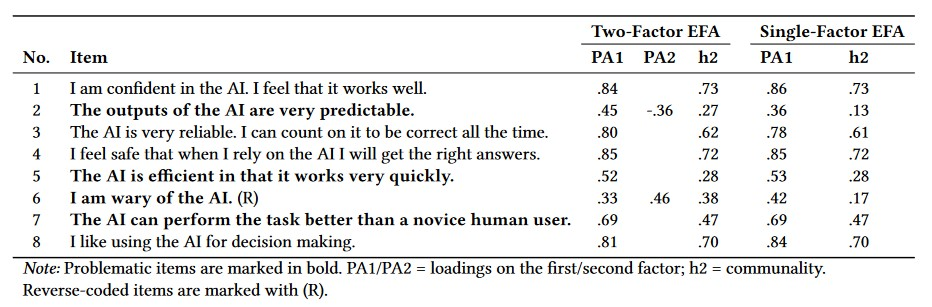
\includegraphics[width=0.8\textwidth]{images/Taken from Perrig et al - Trust tissues with trust scales - review of TXAI by Hofman - 2023.jpg}
  \caption{8 item scale from Hoffman et al \cite{hoffmanMeasuresExplainableAI2023}. As presented in: \cite{perrigTrustIssuesTrust2023}.}\label{fig:CorrectingTXAI}
\end{figure}


Complementary to the assessment of trust, Klein et al. \cite{kleinMinimumNecessaryRigor2023} have set out a framework of 11 requirements by which to guide researchers to run smaller efficient experiments to evaluate human-AI work systems. This new methodology of "Minimum Necessary Rigor" for empirical evaluation of AI is considered necessary in light of the limitations of existing practices which suffer from at the consequence of "rigor mortis": requiring significant funds, large participant pools and complex design and often providing answers no longer required by the time of completion. This method is somewhat contrary to common practice, which promotes the use of a calculating a required sample size for achieving a statistically significant effect on a parametric test \cite{erdfelderGPOWERGeneralPower1996}. This new methodological approach should be being welcomed in light of the voracious pace of AI development, however there is yet any evidence in the literature of its use in practice at time of writing. As such, one should see this proposal as a springboard for discussion, enticing academics to put it into practice and potentially embark on further well scoped, and replicable evaluation methods. Therefore until adequate evidence of its sufficiency is obtained, one should be sceptical until proven otherwise.

In order to build out human centred XAI systems numerous studies and frameworks have been built (\cite{mohseniMultidisciplinarySurveyFramework2021}, \cite{uenoTrustHumanAIInteraction2022},\cite{hoffmanIncreasingValueXAI2023}, \cite{hoffmanMeasuresExplainableAI2023}, \cite{collinsHumanUncertaintyConceptBased2023}) with strong evidence suggesting that feedback modalities with AI systems are key to the their use, with the ability to converse "improving comprehension, acceptance trust and collaboration" \cite{zhangMayAskFollowup2023}. However the use of LLMs as the sole tool for human computer interaction with AI poses significant ethical risks in light of the current lack of XAI methods being deployed \cite{zhaoExplainabilityLargeLanguage2023}.

The fundamental purpose of XAI tools, beyond that of academic research, is that they are intended for practical use in real world domains, in high-stakes decision making, such as medical diagnosis, automated driving, detecting deep-fakes or LLM generated text. This fundamentally requires incorporating the user from inception to deployment. 

High-stakes decision tasks are a prime use case for XAI, yet due to their nature, often problematic to study due to the requirement of developing experiments that are abstracted from the reality.

Examples such as ChatCAD \cite{wangChatCADInteractiveComputerAided2023} demonstrate the possible capabilities in the realm of medical diagnosis and engagement, enabling patients whom may not have access to a doctor the ability to question and garner further insight into their condition. However, ChatCAD has not been discussed nor reviewed by medical practitioners, highlighting the need for far greater interdisciplinary collaboration. 

Leichtmann et al. conducted an exploratory study into the use of XAI \cite{leichtmannEffectsExplainableArtificial2023}, assessing the use of XAI for the high-stake task of deciding if a mushroom is edible or poisonous. The XAI interface delivered an attribution-based example using Grad-CAM \cite{selvarajuGradCAMVisualExplanations2017}, of which the results were statistically significant in improving participants performance in mushroom picking. There are however multiple limitations with this study, such as being restricted to conducting it online rather in the field, and by the sole use of Grad-CAM, of which despite performing better than  LIME \cite{ribeiroWhyShouldTrust2016}, still pertains the intrinsic issues that befall all visual mapping tools.

Alternative XAI methods such as LIME, SHAP, SmoothGrad and Integrated Gradients that are more frequently used have garnered a larger pool of critical research, of which is tackled in the following chapter.

\section{Prior research - the foundation of this project}

To understand the motivations and subsequent approach that this project took, it is necessary for one to grasp the concepts, reasoning, and methodology of the research paper on which it builds upon, along with the limitations therein.

In 2022 Grange et al. \cite{grangeXAISelfexplanatoryAI2022} published a paper presenting a novel methodological approach for constructing an inherently understandable AI. Motivated by the desire to improve AI accountability, increase trust, and adoption, primarily in the high-stakes decision making applications involving health, safety and risk. 

The research approach was primarily grounded in the field of Psychology, drawing upon a body of research conducted by Nosofsky et al. (\cite{sandersTrainingDeepNetworks2020}, \cite{nosofskyTestsExemplarmemoryModel2018}, \cite{miyatsuFeatureHighlightingEnhances2019}) whose expertise and publications in the realm of human categorisation theory had recently highlighted the potential interest of Deep Neural Networks (DNNs) to the field.

Human categorisation theory encompasses various mathematical models, such as mixed representations and rules of the mind(\cite{ashbyNeuropsychologicalTheoryMultiple1998}, \cite{ericksonRulesExemplarsCategory1996}), as well as prototypes \cite{smithThirtyCategorizationResults2000} and exemplars (\cite{nosofskyAttentionSimilarityIdentificationCategorization1986a}, \cite{medinContextTheoryClassification1978}, \cite{kruschkeALCOVEExemplarBasedConnectionist1992}), of which the latter two are grounded upon the notion that categorisation is based upon similarity judgements. Prototype and exemplar model domain research has predominantly been constrained to the use of artificially created categories for systematic assessment and review due to the nature of the complexity of real-world categories. 

Recent advances in DNNs have been employed to predict human similarity judgements \cite{sandersTrainingDeepNetworks2020}, revealing the possibility of shared underlying properties for similarity judgements between AI systems and humans. This subsequently prompted psychologists to further explore the depths of these mutual interpretations. Grange et al. demonstrated this explicitly through a partially feature constrained model, which exhibited a strong correlation with the 8 feature dimensions identified by Nosofsky et al. \cite{miyatsuFeatureHighlightingEnhances2019} and the resultant multi-dimensional scaling (MDS) co-ordinates \cite{sandersTrainingDeepNetworks2020}.

\begin{figure}[H]
  \centering
    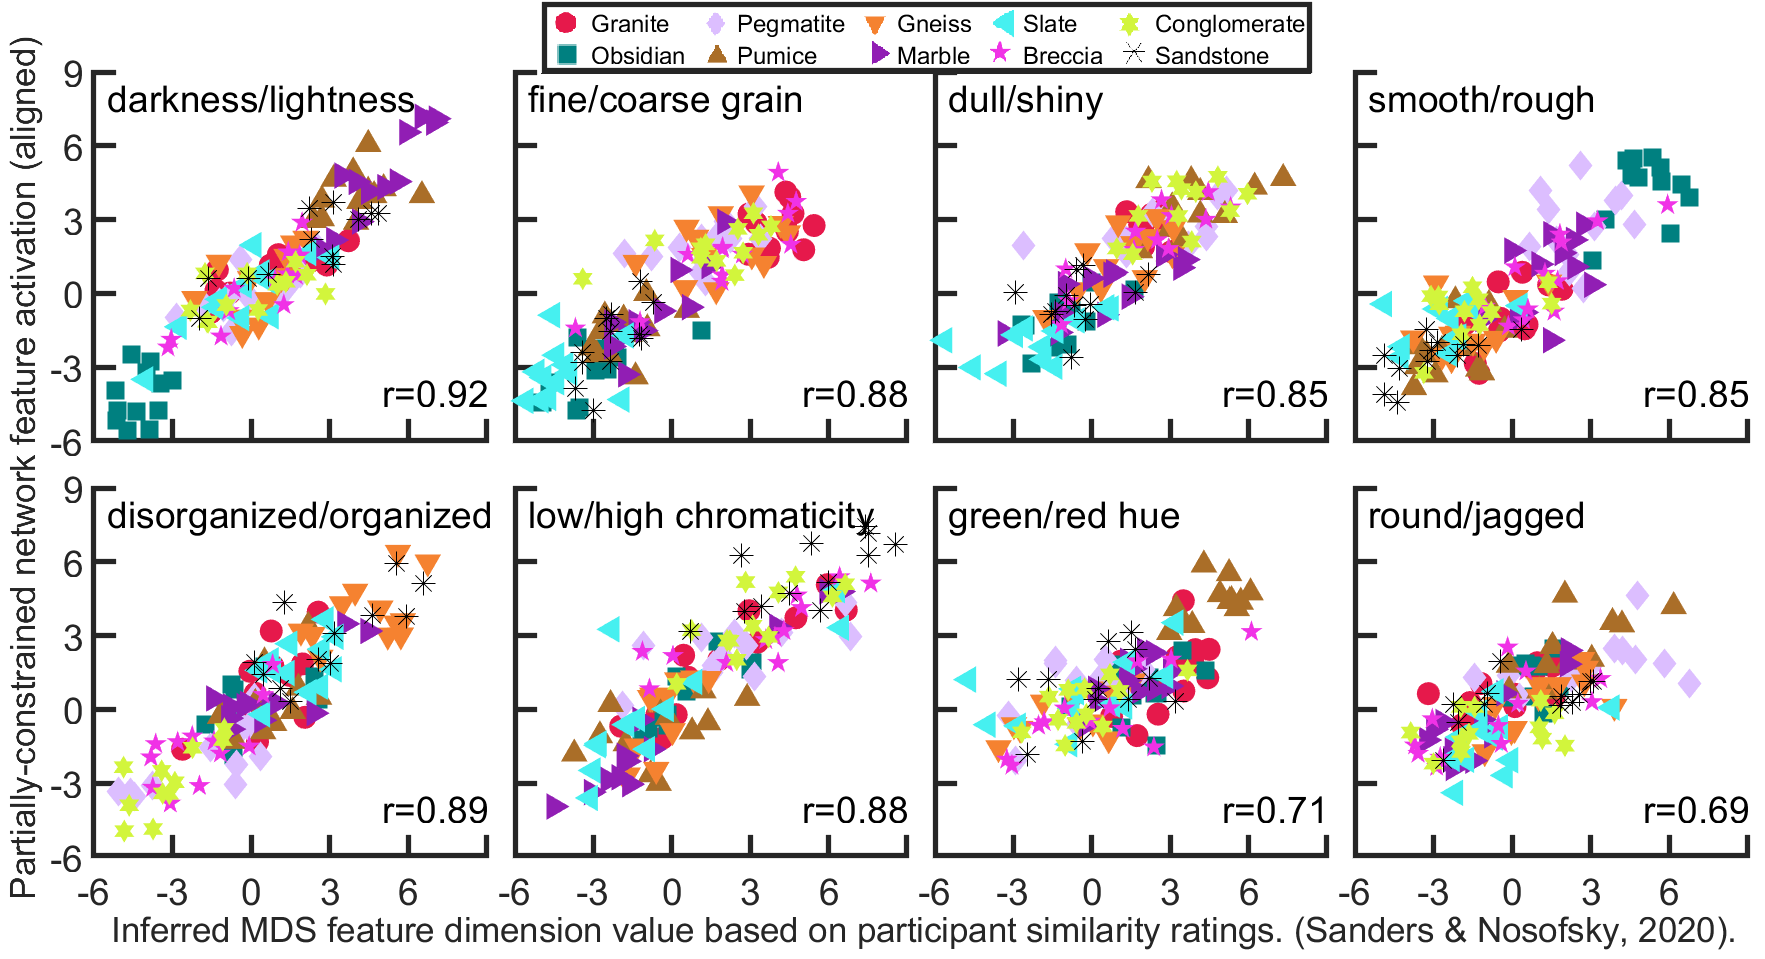
\includegraphics[width=0.8\textwidth]{images/KES2022- MDSvsNetwork Final.PNG}
  \caption{Abstracted features are found to be an affine transform of the Sanders and Nosofsky (2020) inferred MDS feature dimension values based on naïve participants’ similarity ratings. Each plot specifies the MDS feature dimension and the Pearson’s r correlation coefficient. As presented in: \cite{grangeXAISelfexplanatoryAI2022}.}\label{fig:AffineTransform}
\end{figure}

A prerequisite of any explainable and intelligible AI system is the establishment of a shared understanding of concepts. Humans, in general, are less adept at articulating their motivations for categorisation due to complex reasoning, lacking a formal basis on which to do so. On the contrary, domain experts are often intrinsically more adept to do so, equipped with knowledge needed to establish a basis for more profound comprehension of shared concepts between AI systems and experts.

Grange et al. chose the domain of rock classification primarily due to the availability of Nosofsky et al.'s real-world labelled dataset of images and concept/feature ratings, with assessed similarity properties. The similarity judgements from naïve participants enabled the collation of a large database of MDS co-ordinates, from which to input to a low-dimensional similarity space. Due to the high cost of building such a database, Nosofsky et al. circumvented the need to acquire further similarity ratings for new category instances by developing a DNN that successfully predicted MDS co-ordinates \cite{sandersTrainingDeepNetworks2020}.

It's worthy of note that the presence of expert-identified features, from which naïve participants made similarity judgements, expedited participants natural category learning \cite{miyatsuFeatureHighlightingEnhances2019}. As such, further motivating the use of this domain and dataset from which to develop an inherently understandable AI. 

Despite the impressive quality of the ratings data, the collection of rock images was limited in scale when compared to those used to train other AI models e.g. CUB \cite{wahCaltechUCSDBirds2002011Dataset2011}, which comprises of \emph{n} = 11,788 bird photographs. Nosofsky et al.'s set of rock images used in this paper significantly restricted, with 160 "full size" per rock category (n = 1,600), of which 320 random patches were generated and subsequently augmented (translated, flipped, rotated and scaled) to create a set of 480 (n = 4,800).

Thorough employing transfer learning, the penultimate layer of 2048 node activation's (referred to as the "Average Pooling Layer") were  utilised as input into a neural network. These activation's, denoted as  "X train", were combined with a dataset of manually annotated expert feature concepts (Y train), to train the network to predict equivalent expert features. These constrained predicted-feature concepts were subsequently utilised as training data for a single-layer classifier. The fully feature constrained network performed well, achieving a classification accuracy mean of 85.1\% (SD 0.7\%), only 1.7\% short of an unconstrained network’s accuracy mean of 86.8\% (SD 0.8\%).

\begin{figure}[H]
  \centering
    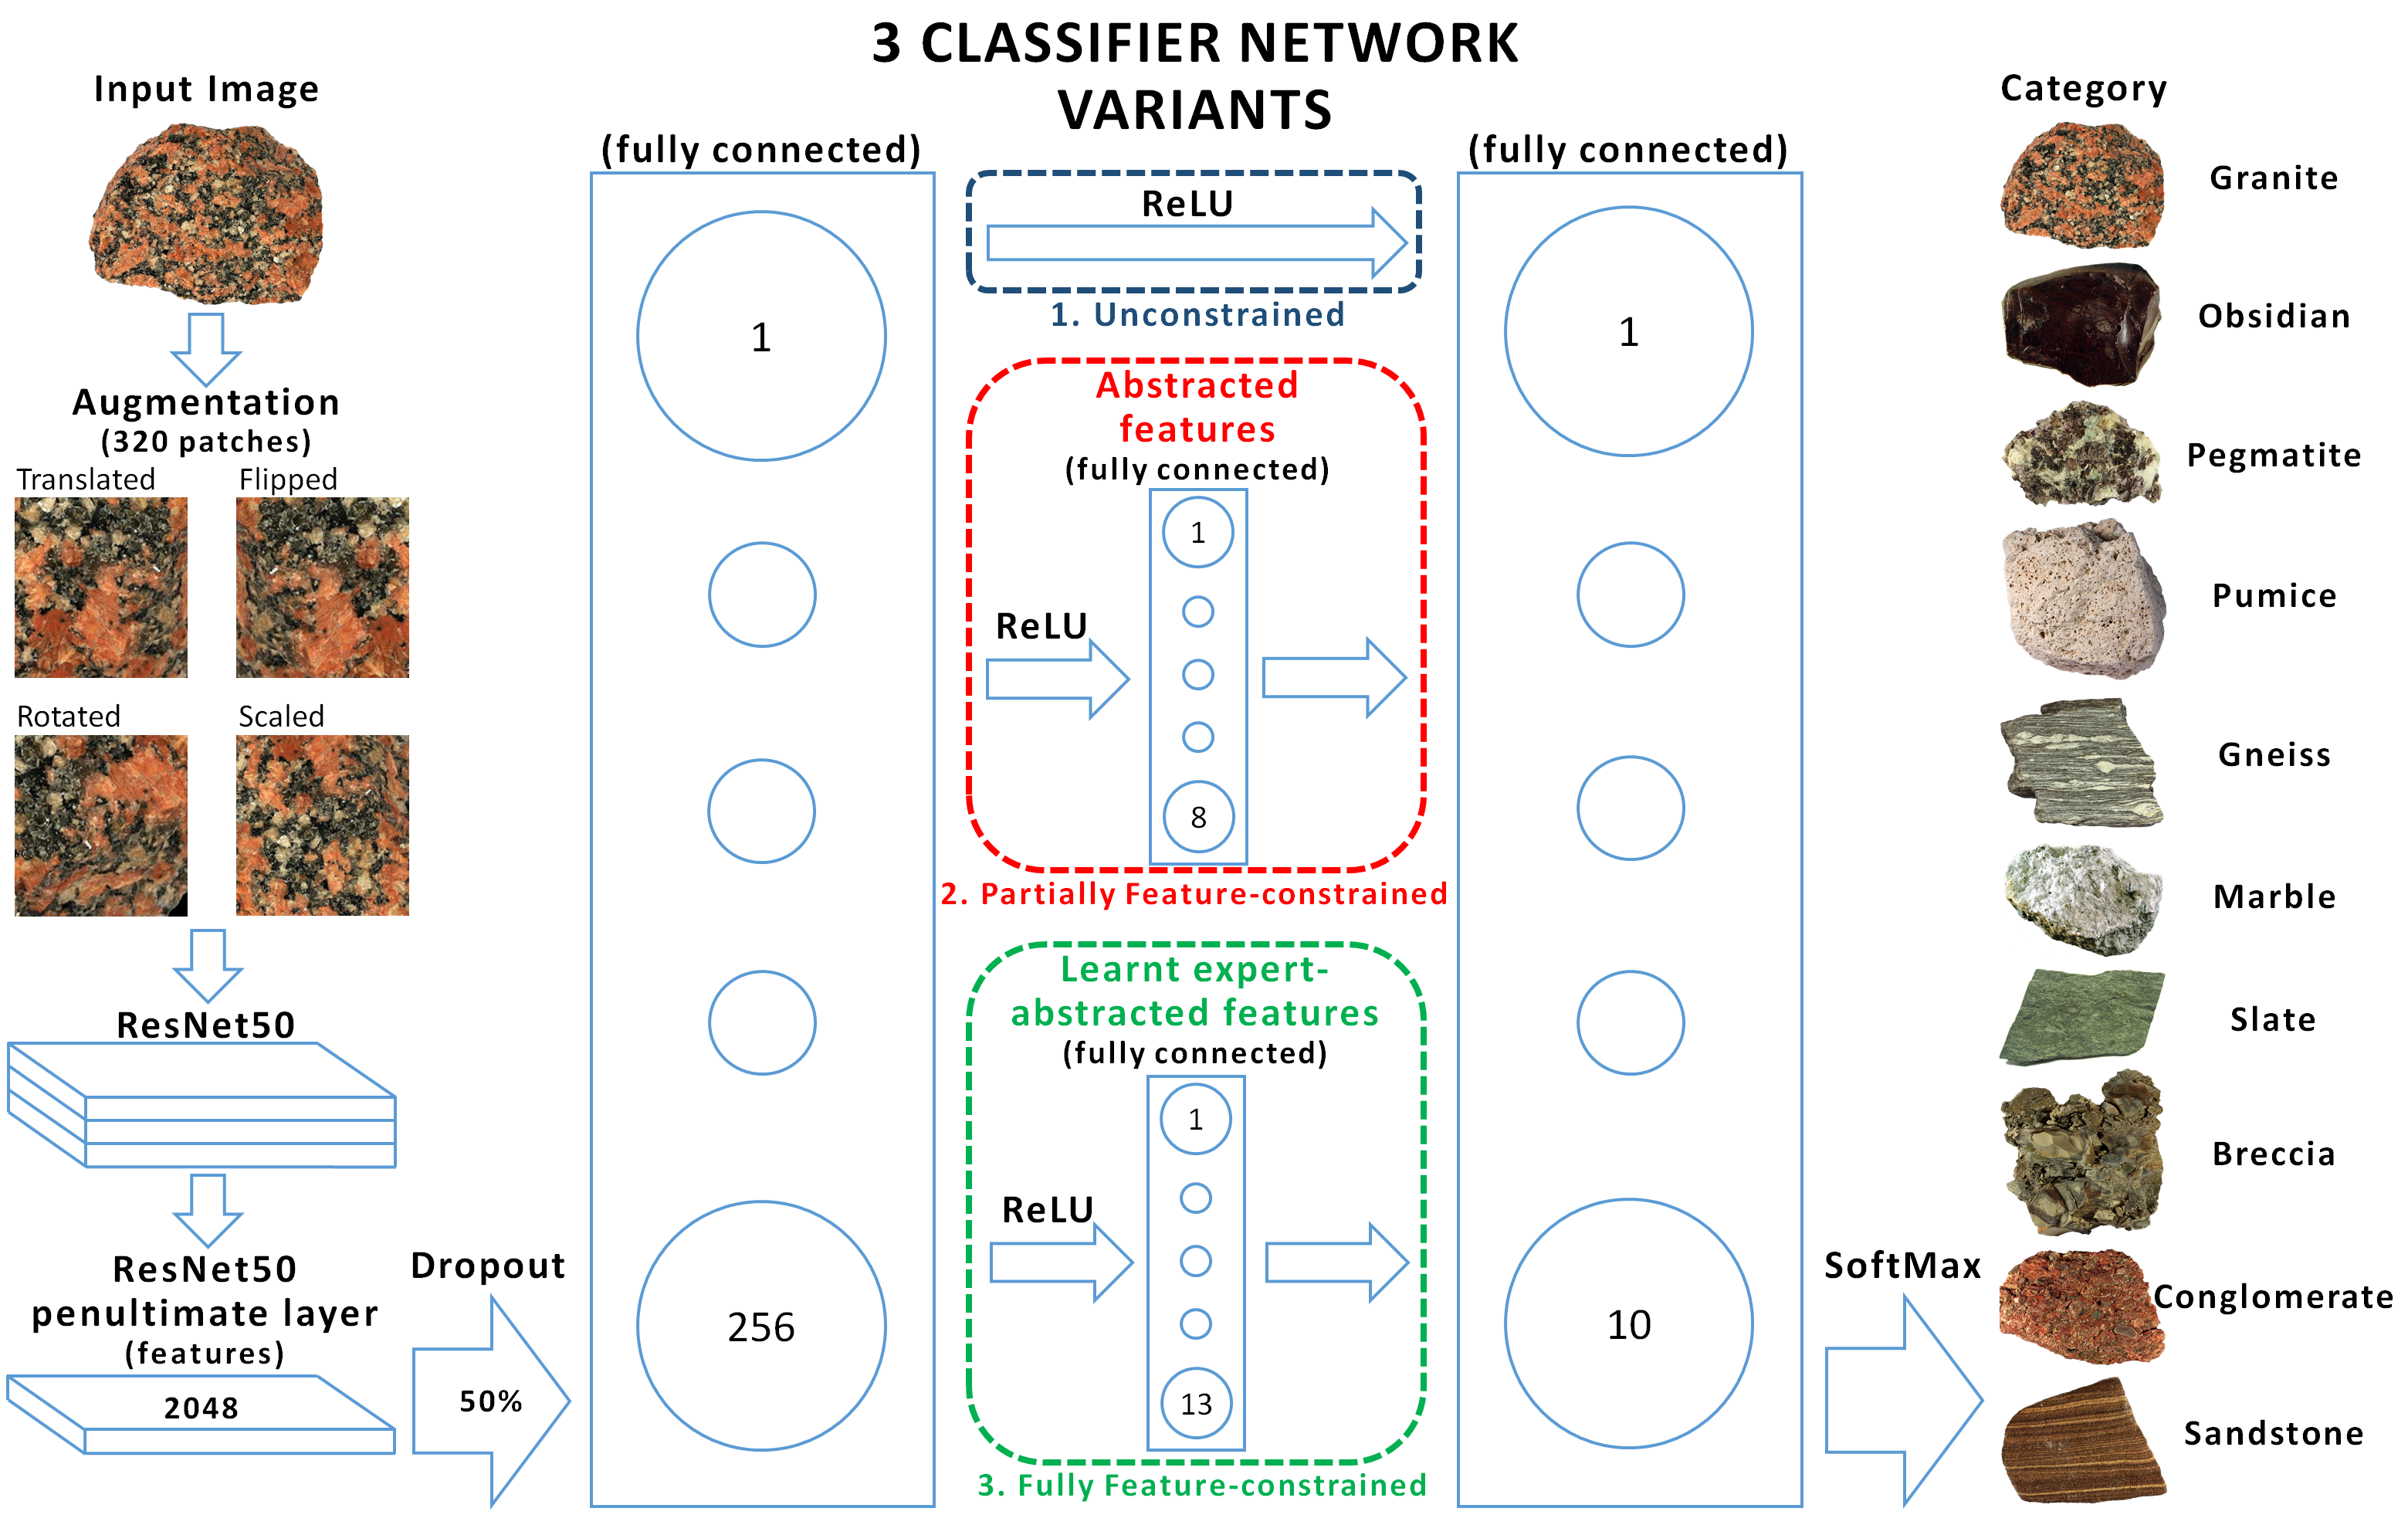
\includegraphics[width=\textwidth]{images/Figure1 - Networks 1-3.png}
    \caption{Illustration of the three classifier network variants making use of transfer learning with Renset50. Rock images are first augmented before being fed through Resnet50, the penultimate layer of Resnet50 is taken through a 50\% drop-out layer, a fully connected 256-node layer, then one of three paths before a 10-node category activation layer is passed through a SoftMax function: (1) an unconstrained variant path, where the 256 node layer fully connects to the 10-node layer through a ReLU function, (2) a partially feature-constrained variant path, where the 256-node layer activations are condensed, via a ReLU function, down to an 8-node, ‘Abstracted Features’ layer and (3) a fully feature-constrained variant path, where the abstracted feature layer is forced to be made of transfer-learned expert-abstracted features. As presented in: \cite{grangeXAISelfexplanatoryAI2022}.}\label{fig:Networks 1-3 XAI&I}
\end{figure}

The finding that an accuracy mean accuracy gap of only 1.7\% between that of the constrained and unconstrained black-box model is impressive. There is however a lack of analysis of features, assessing if any may overlap in knowledge representation, particularly when the correlation between the expert feature ratings and the predicted feature ratings is below that of those which highly correlate e.g. “Brightness Heterogeneity” (r=0.43) compared to “Roughness” (r=0.92).  Further review is also required to understand the nature of features that are rated in a continuous scalar fashion (soft coded) i.e. “Average Grainsize”, compared to that of those with binary ratings (hard coded) e.g. “Presence of Crystals”. A considerable body of research in similar methods shall be critiqued in this dissertation, in support of both binary and scalar methods of coding concepts. 

This begs the question of whether DNNs are interpreting non-binary concept/feature ratings beyond binary distinctions, as many of the features in this model lean towards continuous ratings. However, one should consider if the DNN is perceiving features that are visible in the image or features that are intrinsic to the category/classification type. For example, “Granite” always contains crystals, yet the extent to which they are present may not be equally visible from every image angle.

\section{A Review of Relevant and Recent XAI Methods}

As XAI developers and researchers alike strive to develop new insight and tools with the aim of delivering improvements on the interpretability and explainability of models for a wide variety of users, there ultimately lies a distinction between which route they choose to take to deliver on these promises. This varies dramatically based upon the domain scope (local or global), stage (ante-hoc or post-hoc) and the output format (numerical, visual, textual or mixed) \cite{yangSurveyExplainableAI2023}.

Chen at al. \cite{chenConceptWhiteningInterpretable2020} propose defining interpretability and explainability methods based upon stage alone:
\begin{enumerate}
    \item Ante-hoc, inherently interpretable models (\cite{chenConceptWhiteningInterpretable2020}, \cite{kohConceptBottleneckModels2020}, \cite{havasiAddressingLeakageConcept2022a}, \cite{rudinInterpretableMachineLearning2021}, \cite{eltonSelfexplainingAIAlternative2020}, \cite{grangeXAISelfexplanatoryAI2022})
    \item Post-hoc explanations for existing neural networks (\cite{ribeiroWhyShouldTrust2016}, \cite{lundbergUnifiedApproachInterpreting2017},\cite{zeilerVisualizingUnderstandingConvolutional2014},\cite{simonyanDeepConvolutionalNetworks2014}, \cite{smilkovSmoothGradRemovingNoise2017}, \cite{selvarajuGradCAMVisualExplanations2017})
\end{enumerate}

The majority of XAI methods fall into the category of post-hoc explanations, with vastly different levels of explanation given with equally as wide levels of comprehensibility. Post hoc methods, such as heat maps and saliency maps (\cite{ribeiroWhyShouldTrust2016}, ,\cite{zeilerVisualizingUnderstandingConvolutional2014},\cite{simonyanDeepConvolutionalNetworks2014}, \cite{fongInterpretableExplanationsBlack2017},\cite{smilkovSmoothGradRemovingNoise2017}, \cite{selvarajuGradCAMVisualExplanations2017}, \cite{sundararajanAxiomaticAttributionDeep2017}), being the most common and often used within industry \cite{holzingerXxAIExplainableAI2022a}. 

\begin{figure}[H]
  \centering
    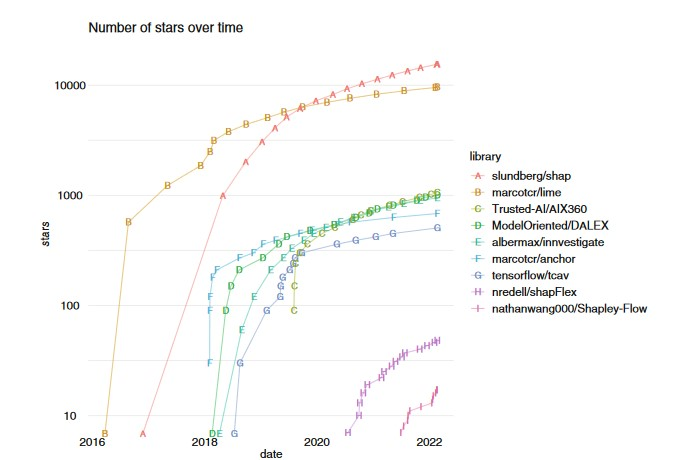
\includegraphics[width=0.8\textwidth]{images/most popular XAI toolboxes - GitHub Stars - xxAI 2022.jpg}
  \caption{The most popular XAI repositories on GitHub (number of stars) as presented in: \cite{holzingerXxAIExplainableAI2022a}.}\label{fig:Popular XAI Tool}
\end{figure}

This methodological approach tackles the delivery of an explanation by weighting each pixel of an input image, producing a visual image of to the end user, with the aim of showing the importance each pixel made to the final classification. This can be problematic, as many of these methods can only highlight the edges of an image, offering little of use in terms of an explanation i.e. the differences between one class and another (\cite{rudinStopExplainingBlack2019}. Saliency maps are also prone to to sensitivities in the data or model, and as such, potentially misleading if used as a sole means of assessment \cite{adebayoSanityChecksSaliency2018a}.

The misleading nature of saliency maps is supported by Kim et al. \cite{kimInterpretabilityFeatureAttribution2018} in an experiment measuring the perceived importance of an image and concept. Participants were shown four images with concept captions (produced using Concept Activation Vectors \cite{kimInterpretabilityFeatureAttribution2018}), each with two corresponding saliency maps (SmoothGrad \cite{smilkovSmoothGradRemovingNoise2017} and Integrated Gradients \cite{adebayoSanityChecksSaliency2018a}) and asked to rate the importance of the image to the model (10-point Likert scale), the importance of the caption (10-point Likert scale), along with their confidence in their answer (5-point Likert scale). The results indicate that due to the percentage of correct answers rated as very confident being equivalent that of incorrect answers, that saliency maps have a tendency to be misleading. There was also a degree of decorrelation in accuracy between the two saliency maps i.e. when one correctly communicated a concept, it was not always true with that of the other. This further supports the notion that post-hoc saliency methods are frequently fragile and limited in their ability to deliver a useful, explanation. This supports the need for inherently interpretable models, of which this research project attempts to tackle.

\subsection{Concept Bottleneck Models}

The emergence and growth in research on Concept Bottleneck Models (CBMs) has been motivated with two key benefits in mind when approaching the task of XAI. Firstly, there is the promise that class classification predictions can be explained using high-level human interpretable concepts produced by a concept predictor \cite{grangeXAISelfexplanatoryAI2022}. Secondly, that a human operator can intervene, altering concept values and monitoring the effect this has on the final prediction \cite{havasiAddressingLeakageConcept2022a}. 

One of the first propositions in this field was that of “Concept Whitening”(CW) \cite{chenConceptWhiteningInterpretable2020}. This purportedly inherently interpretable model, places a bottleneck in a CNN, replacing a batch normalisation (BN) layer with a novel CW layer. By doing so, the latent space of a neural network is “disentangled”, constraining the neurons in the network to realign to the axes of predefined concepts understandable by humans. The research method uses ResNet18, with experiments conducted that assert that the 16th layer provides the clearest approximation of concept alignment. This focus on the penultimate layers of the model, is congruent with the idea that higher-level semantic concepts are present in the latter layers of CNNs (\cite{zhouInterpretingDeepVisual2017}, \cite{grangeXAISelfexplanatoryAI2022}). All experiments using this combination are trained using the Places 365 dataset, with either three or seven simultaneous concepts from the MS COCO dataset.  

It can be argued that the concepts being defined here are quite primitive and limited in dimensionality e.g. “air-plane”, “bed” or “person”, and as such fail to deliver, beyond that of the clarity of a single concept in an image, and is somewhat analogous to a "grandmother cell" in neuroscience. It therefore falls short of denoting the deeper semantic descriptors of an images features e.g. if the image is that of an  air-plane, why is it so? Presence of wings, flying in the sky, shape etc. Rather the output focuses on what it is not e.g. an air-plane is not a table, bed or boat. This is a clear limitation of the training data used (Places 365 \& MS COCO), of which is such granular details are not inclusive. Consequently, the paper concludes, that if a full explanation on each computation were to be delivered then this would lead to a restriction on flexibility, however one may determine that the complexity would be considerably reduced if only applied within an a single expert domain. The transference of the CW model to an expert domain is attempted, focusing on skin lesions, however it is limited by the use of only two concepts, age and legion size, of which age is discovered to play no importance to classification. Opposingly, the size of the legion (>=10) is in the third quartile of importance (of 512 axes), a concept that is know to be used by physicians for diagnosis of skin lesions \cite{walterUsing7pointChecklist2013}. This brief insight into the importance of expert domain knowledge reinforces the need for the incorporation of well defined concepts based upon existing empirical evidence, reinforcing the body research undertaken in this project.

The pursuit of a delivering a comprehensive explanation has led to the prolific development of new concept bottleneck models (CBM), both ante and post-hoc (\cite{kohConceptBottleneckModels2020}, \cite{margeloiuConceptBottleneckModels2021}, \cite{havasiAddressingLeakageConcept2022a}, \cite{yuksekgonulPosthocConceptBottleneck2022}). 

Koh et al. \cite{kohConceptBottleneckModels2020} offer three CBM models for exploration: 
(1)	Independent bottlenecks, whereby concepts and classification are learnt in separate algorithms, with the resultant learnt concepts used for classification at test time.
(2)	Sequential bottlenecks, whereby the concept is learnt, with the learnt concepts used to inform classification learning.
(3)	Joint bottlenecks, whereby the concept and classification are both learnt in combination during training, whereby $\lambda$ regularisation factor is adjusted using the combined losses  

The findings illuminate that not only by using human annotated data for training, but along with the intervention by an expert (particularly independent bottlenecks), a model can be updated if an artefact is incorrectly identified as a concept/feature, substantially improving accuracy beyond that of a standard model, with an overall observation that there is not in fact a trade-off between high task accuracy and high concept accuracy \cite{kohConceptBottleneckModels2020}.

Due to the improved levels of predictive performance (analysis of Root Mean Squared Error - RMSE) through concept refinement, Koh et al. take preference to the proposed joint CBM model. Yet it is noted that the benefits of intervenability in joint models is detrimental to performance. To the contrary, independent models benefited the most from expert intervention of concept prediction using ground truths.

The quality of the output of all three models proposed by Koh et al. is interrogated by Margeloiu et al.'s \cite{margeloiuConceptBottleneckModels2021} three desiderata of a CBM:
1.	Interpretability: Being able to note which concepts are important for the targets. 
2.	Predictability: Being able to predict the targets from the concepts alone. 
3.	Intervenability: Being able to replace predicted concept values with ground truth values to improve predictive performance.

The methodology used by Margeloiu et al. to critique Koh et al.’s three CBM models, requires the development of a concept oracle model (CO); a model using ground truths to predict target images. The CO is used to compare through the correlation of the root mean square error (RMSE) of each CMB model and CO. The finding suggests that independent CMBs and COs have a far higher coefficient of determination. This observation aligns with the hypothesis that predicted concepts (as per sequential and joint CBMs) are not used as intended, but rather as proxies to incorporate target information, shown with a vastly reduced RMSE as the level of concept intervention increases, particularly that of independent CBMs (see Fig 4 in \cite{kohConceptBottleneckModels2020}). It is suggested by Margeloiu et al. that one of the reasons for low correlation of concepts in sequential and joint CBMs to COs is a result of the use of one-hot encoding for concept values i.e. concepts are binary (0 or 1). Leading on to suggestions of further study, through the analysis of the variability of concept representations by means of binary and scalar concepts, and one-hot encoded categoricals. It should be noted that some analysis of binary and scalar concepts is tackled later on within this research project manuscript. Margeloiu et al. also take on the use of saliency maps (Integrated Gradients with Gaussian Noise baseline) to try and assess the predicted concepts visually, showing attention across the whole image rather than that of the defined feature, however, as commented by many others, saliency maps are unable to map concepts in any meaningful manner (\cite{rudinStopExplainingBlack2019}, \cite{adebayoSanityChecksSaliency2018a},\cite{kimInterpretabilityFeatureAttribution2018}).

\subsection{Post-hoc Concept Bottleneck Models}

Complementary to the development of CMBs, much research has been undertaken in the development of post-hoc CBM (PCBM) methods (\cite{havasiAddressingLeakageConcept2022a}, \cite{yuksekgonulPosthocConceptBottleneck2022}, \cite{daneshjouSkinConSkinDisease2022}), of which attempt to address multiple issues, such as the loss of concept clarity or “leakage” \cite{mahinpeiPromisesPitfallsBlackBox2021}. It is speculated that the cause of leakage may be the result of an overlap of concepts in the concept predictor layer due an insufficient concept set being available e.g. some classifications may require more concepts than others, or that “soft” concepts i.e. non-binary concepts (probabilities, often between 0 and 1) allow unintended information to be conveyed. In conclusion, resultant leakage muddies both interpretability and the ability to effectively intervene on the concept predictor. The alternative to soft CBMs is that of hard CBMs, whereby concepts are binary. One may consider this approach to be more truthful, as leakage between concepts is prevented, yet this method is prone to lower classification accuracy unless all concept details are captured correctly. There is no flexibility for the system to leak knowledge into another concept, thus  thorough domain knowledge is required to prevent miscoding concepts, either by not getting the quantity correct, through human error in labelling the training data, or a mutual lack of understanding between the user, the domain, the input, and the models deliverables (perhaps there is hidden knowledge the model requires that is not innately intelligible by humans). This notion is contrary to the supposition by Margeloiu et al. that hard CBMs may be responsible for the low correlation of concepts in sequential and joint CBMs. 
A conclusion may be drawn that naturally, some concept features could always be considered binary due to their intrinsic nature e.g. obsidian rocks will always have a glass like texture, or marble being composed of crystals. However, it is less clear if the network would benefit from further granularity, i.e. how much of said concept is present in the image used for training.

Havasi et al. \cite{havasiAddressingLeakageConcept2022a} propose two further means of addressing leakage and improving performance of hard concept CBMs: (1) a side channel model and (2) an auto-regressive architecture. Prior to using either tools a model is first analysed to see if the concepts are sufficient in predicting the final label classification, or if more information is desired – the lack of a Markovian assumption. The side channel model is a small single layer which is trained concurrently with the hard CBM from a set of latent concepts, with the flexibility to infer how many concepts are required for label prediction. This side-channel enables one to estimate the completeness of the original concepts, and therefore can be used as a form of diagnosis to infer if there are key concepts missing. Yet, on closer inspection it is clear that much of the side channel information has the propensity to deliver concepts uninterpretable by humans – something that may or not be desirable depending upon the domain and accuracy required by the end user. The second tool is that of an auto-regressive architecture that allows for hard CBMs to learn correlations between concepts, therefore re-weighting concepts, with interventions also affecting concept predictions of prior concepts. They note that normalisation is of upmost importance to ensure that correct predictive distribution. Both methods come at the cost of increased  computation; however they do put hard CBMs at an accuracy level equivalent to that of soft CBMs. This may be desirable in some domains whereby concept knowledge is always translatable in a binary manner, however in many domains this is not always the case, and if applied then the initial mandate, to enable human interpretability, is lost.

A novel post-hoc CBM (PCBM) model is proposed by Yuksekgonul et al. \cite{yuksekgonulPosthocConceptBottleneck2022}, attempting to tackle three key limitations of CBMs: access to data i.e. the laborious task of annotating or collating a concept dataset, increasing performance, and the enablement of intervention by human input. The first task of collating a concept databank is approached in two ways, through utilising Concept Activation Vectors (CAVs) or with state of the art (SOTA) multi-modal models such as "Contrastive Language Image Pre-Training" (CLIP) \cite{radfordLearningTransferableVisual2021}. 
The use of a CAV is utilised by learning concepts selected by a domain expert, or automatically from the data, that positively or negatively associate with the image. This method is pragmatic in that it does not require the training data to mirror the data used to train the backbone model, as per requirement of a CBM. A linear standard vector model (SVM) is then used to learn the corresponding CAV, using the positive and negative examples to denote the vector notal to the linear classification boundary.

The second method for constructing a concept bank is through the utilisation of the text encoder from the multi-modal model CLIP, of which contains both text and image encoders to map a description to a shared embedding space. A concept description vector is obtained through collating the relevant text embeddings to be utilised in combination with an open knowledge graph, ConceptNet \cite{speerConceptNetOpenMultilingual2017}, to collate the relationships between classes and concepts. 

Once a concept subspace is learnt through either CAV or CLIP, a sparse linear model or decision tree is used for prediction due to the inherent clarity and insight with which one can observe a decision being made. It is noted that the richness of the concept subspace is important to the performance accuracy of the PCBM, of which would no doubt disincentivise any potential user for uptake over that of a normal model. An attempt to solve this issue is made by utilising a sequential residual predictor, that attempts to retain some of the original model’s accuracy, a concept denoted as Hybrid Post-hoc CBMs (PCBM-h). Despite this effort to debug the CBM model, there is still the  risk that one may be limited with a poor concept library, ill equipped to express and solve the task it is required, and potentially containing and reinforcing biases. Despite this, Daneshjou et al. \cite{daneshjouSkinConSkinDisease2022} successfully incorporates the PCBM methodology into a novel work flow, using expert dermatologist defined concepts to develop SkinCon. A dataset of existing image annotations was used, and clarified using expert intervention..

Others have approached the matter of concept completeness/sufficiency and discovery in alternative means, such as ConceptSHAP \cite{yehCompletenessawareConceptBasedExplanations2019}. Yeh et al.’s method delivers a completeness score, shedding light on how sufficient concepts are for delivering an explanation, along with a means of to alight how important each concept is to an input by adapting the widely used Shapley value method \cite{shapley17ValueNPerson1953}. The method uses concepts that are common across all classes as opposed to one, postulating that shared class concepts are useful for interpretation of the model, e.g. one may determine through analysis of the concepts by nearest neighbour, that the shape of an animal’s head is important and shared between multiple classes. In an expert domain, the idea of shared concepts is often common place due to the scope being local rather than global. A quick alternative to this method, often used, is to calculate the L2 norm of a the weights in a model to deride which features are most important. However, unlike Shapley values, L2 norm cannot capture the nuanced interaction between individual features in the same way. As such, the incorporation of ConceptSHAP into the realm of CBMs is arguably a vital addition to the AI and ML practitioners toolbox.

\subsection{Concept Bottleneck Models and Large Language Models}

SOTA CBMs have begun leveraging the use of Large Language Models (LLMs), such as aiding with the laborious task of annotating data sets. Language Guided Bottlenecks (LaBo) \cite{yangLanguageBottleLanguage2023}, does so by aligning GPT-3's sentence based concepts using CLIP to form a bottleneck layer. There are some limitations, such as fine tuning the output of GPT-3, restricting the sentence length, and preventing the use of class names. Yet this is arguably preferable as the generated concepts can be controlled and chosen based upon a number of factors, such as interpretabilty, classification accuracy, and those which are highly discriminative and recognisable by CLIP. As such, this model strongly leans towards the the classification of being ante-hoc/inherently interpretable, as it essentially focuses on the fine tuning of CLIP. However the performance is restricted by the training data of GPT-3 (at least in this iteration), which excels in common categories, yet rapidly falls short with delivering higher granularity in more nuanced fields of enquiry, reducing it's potential use case for a number of expert domains. The concept of integrating LLMs, despite being out of the remit of this project, is one of significant future interest, particularly with the development of new LLMs that can be fine tuned to focus on specific expert domains. Yet, as previously noted, LLMs are vastly more difficult to explain in comparison to current NN methods, requiring whole new methodologies in the realm of XAI \cite{zhaoExplainabilityLargeLanguage2023}.  

Other developments incorporating LLMs explore the incorporation of multiple models and multiple input modalities e.g. ChatCAD \cite{wangChatCADInteractiveComputerAided2023} for medical image diagnosis. ChatCAD leverages multiple SOTA computer aided diagnosis (CAD) networks e.g. a disease classifier, lesion segmentor, and report generator, from which a combined prompt text can be generated for input into an LLM such as ChatGPT. In doing so a condensed report of the diagnosis is produced, leveraging the the models knowledge of the medical field \cite{gilsonHowDoesChatGPT2023}, and enabling the user to interrogate the report through conversational enquiry. 

Zhang et al. \cite{zhangMayAskFollowup2023} support the notion of free-form conversation with a network, demonstrating that comprehension, acceptance, trust and collaboration are significantly improved between the user and AI model. However their experiment is not without limitations, such as the use of the wizard-of-oz methodology and only two two feature attribution tools (LIME and Grad-CAM) being used as a means of explanation (the limitations of which have previously been stated).

Further developments in multi-modal LLMs such as NExT-GPT \cite{wuNExTGPTAnytoAnyMultimodal2023} indicate the possibility to deliver upon potentially higher levels of explainability as well as inclusivity via the use of modality switching e.g. from natural language text, to image, video or audio, subsequently delivering a more human like means of interaction. NExT-GPT does so by the use of modality-switching instruction tuning (MosIT), in combination with a manually curated high quality dataset. Despite the impressive possibilities of this model (requiring only 1\% of the parameters to be updated during training for each new modality), with hopes of incorporating additional modalities in its next iteration e.g such as tables, figures, heat maps and so on; the manual curation of a bespoke dataset (MosIT) is somewhat concerning. As with all data sets, there is always the risk of human bias being encoded, unconsciously or otherwise, through the selection of data and its subsequent annotations. This further highlights the need for legislation and the regulation of data used to train such models. 

With the ever increasing complexity of AI systems that combine multiple models and modalities (\cite{wangChatCADInteractiveComputerAided2023}, \cite{wuNExTGPTAnytoAnyMultimodal2023},\cite{yangLanguageBottleLanguage2023}), it will become an ever increasing challenge to incorporate explainability and interpretabilty throughout. Therefore, the use of accurate, explainable, and interpretable CBMs hold a strong defence to be included as an essential item in a developers toolbox when delivering a trustworthy complex AI system, offering a glimmer of transparency, in light of other elements which may appear opaque.
\chapter{Approach, Methodology and Results}
\section{Approach}

The approach to enhancing network accuracy whilst preserving human aligned concepts, was formulated through a series of informal discussions with departmental colleagues and co-authors as noted in \cite{grangeXAISelfexplanatoryAI2022}. Consequently, both I and others, were already invested in the idea, so the decision to commit to the further utilisation of the existing model that had been researched and developed made logical sense. The decision to approach the project using this existing constrained sequential CBM and expert-rated data set \cite{grangeXAISelfexplanatoryAI2022} as a starting point provided me with the advantage of being able to meet the aims and objectives of the dissertation within the given time frame, without building a network from scratch.

The use of this model and subsequent dataset also had the distinct advantage of empirical evidence for the validity of the feature concepts in the research conducted by Nosofsky et al. (\cite{nosofskyDevelopmentFeaturespaceRepresentation2018}, \cite{miyatsuFeatureHighlightingEnhances2019}, \cite{sandersTrainingDeepNetworks2020})., The data set was also unique in its use of combining both \emph{soft}, information rich, scalar concepts (in this instance between 1 and 9), and \emph{harder} binary concepts (1 or 9). The reasoning for using a scale of 1-9 is rooted in the initial dataset of MDS co-ordinates from Nosofsky et al. It was, and remains, unclear if this a-typical method of rating feature concepts improves performance in comparison to other \emph{soft} CBM models, of which use probability ratings between 0-1. It is also worthy of noting that in previous iterations of the network (in the build up to \cite{grangeXAISelfexplanatoryAI2022})  that a model gradients function was used, penalising any feature concepts that were rated as -1 i.e.  not present. However this method of rating concepts was removed due to the analysis showing a reduction in the accuracy of classification and weak concept alignment. Evidence in the literature for improved classification accuracy when using \emph{soft} scalar concepts has been pointed to as a potential result of information \emph{leakage} \cite{havasiAddressingLeakageConcept2022a} i.e. soft concepts may be misrepresenting the data, and therefore muddying the interpretability of the model. Yet with binary concepts, despite being more truthful, they often penalise the accuracy of the classification. This has been hypothesised as a potential result of the lack of required concept features needed by the model. The discovery of this in the literature only served to strengthen my initial thoughts on the matter and concluded that it was a worthy avenue of research within this project. 

Amongst other proposals considered, was that of joint training through a combined loss function, akin to Koh et al. \cite{kohConceptBottleneckModels2020}. However, I believed there was a pressing need for a deeper understanding of what the existing sequential CBM model had learnt with regards to the validity of the concepts. This was further supported by claims from Margeloiu et al. \cite{margeloiuConceptBottleneckModels2021}  that joint CBMs have a tendency towards a low correlation of concept values, and that the benefits that may be had from intervention are in fact detrimental to performance.

The desire to understand more about the sequential CBM developed by Grange et al. and the concepts it had learnt, eventually fostered the novel idea that the weights and biases (\emph{w} + \emph{b}) learnt by the existing CBM \cite{grangeXAISelfexplanatoryAI2022} could be used to initialise a new CBM classifier. The decision to take this approach was based on the notion that by giving the network some additional degrees of freedom to learn, greater classification accuracy may be achieved (akin to that of a black box) whilst regaining the existing highly correlated expert feature values. Additionally, the appended hybrid network could serve as a tool for assessing the quality of the learnt expert feature values in the sequential bottleneck model via comparative correlation. In turn, allowing the user to intervene with the training data.

The framework of the approach adopted comprised of the following steps: 

\begin{itemize}
\item Utilisation of the model proposed by Grange at al. 2022 \cite{grangeXAISelfexplanatoryAI2022} as a foundational starting point

\item The development of an additional network classifier that employs the acquired knowledge embedded within the weights and biases of the previous CBM model \cite{grangeXAISelfexplanatoryAI2022}. Implementation in MATLAB \cite{MATLAB}, following the methodology of the previous model, will expedite development and subsequent data collection

\item Developing analytical tools with which to appraise the classification accuracy and concept alignment of the new hybrid classifier to that of the prior CBM and to the expert training data

\item Quantifying the effects on classification accuracy and concept alignment when using binary or continuous concept/feature ratings

\item Evaluating the impact on classification accuracy when removing a concept/feature with low correlation to the input dataset of human intelligible features

\item Investigating the outcomes on classification accuracy and concept alignment through the manipulation of network learning variables, such as the number of epochs, mini-batch size, and learning rate

\end{itemize}

Throughout the project an ongoing literature review was conducted in order to keep abreast of new developments in the field of XAI. The lack of clarity with regards to terminology in the domain was a considerable hindrance during the development of the initial sequential CBM \cite{grangeXAISelfexplanatoryAI2022}. As such it was essential that I made a continued effort to build a repository throughout the project to inform my decisions and prevent the replication of research already conducted in previous studies. I found many examples of post-hoc CBM methods (\cite{havasiAddressingLeakageConcept2022a}, \cite{yuksekgonulPosthocConceptBottleneck2022}, \cite{daneshjouSkinConSkinDisease2022}), and others that addressed the loss of concept clarity or “leakage” \cite{mahinpeiPromisesPitfallsBlackBox2021}, however I did not find evidence of the methodology as proposed in this work, being replicated elsewhere.

\section{Design and Implementation}

The development of the hybrid classifier network was completed in Matlab as planned. A snippet of the code can be see below:

\lstinputlisting[language=Matlab,firstline=559, lastline=605, caption= Matlab code for the Hybrid Network Classifier]{Code/networksAll.m}

The design developed continues the use of transfer learning as per \cite{grangeXAISelfexplanatoryAI2022}, taking in the 2048 features from ResNet50, with a 50\% dropout layer, in line with the previous CBM design. However, where the new hybrid classifier differs is in that the three fully connected layers are initialised with the weights and biases (\emph{w} + \emph{b}) learned from the constrained sequential CBM (see Figure ~\ref{fig:Hybrid classifier XAI&I}). The first fully connected layer consists of 256 nodes which are not allowed to learn (with a learning rate of $\eta$ = 0). In contrast, the subsequent fully connected layers, of 13 nodes in the concept layer and 10 nodes in the classification layer, are free to do so (with an initial learning rate of $\eta$ = 0.001). This flexibility in the model to deviate along only two of the feature layers (concept and classification layers), using the same number of nodes as per the previous CBM (except for the case of one experimental method of removing one concept, and subsequently one node in the concept layer), made it possible to evaluate the results against both the original CBM and the expert training data. This design ensured that the resultant concept features were prevented from straying too far outside of the bound of 1-9, as per the original training data.

One may view the hybrid classifier as an extension of a sequential CBM, due to the manner in which it relies upon the weights and biases of the preceding network classifier, thus in reference to the terminology used in the literature one could pertain that this model functions as a post-hoc sequential CBM.

\begin{figure}[H]
  \centering
    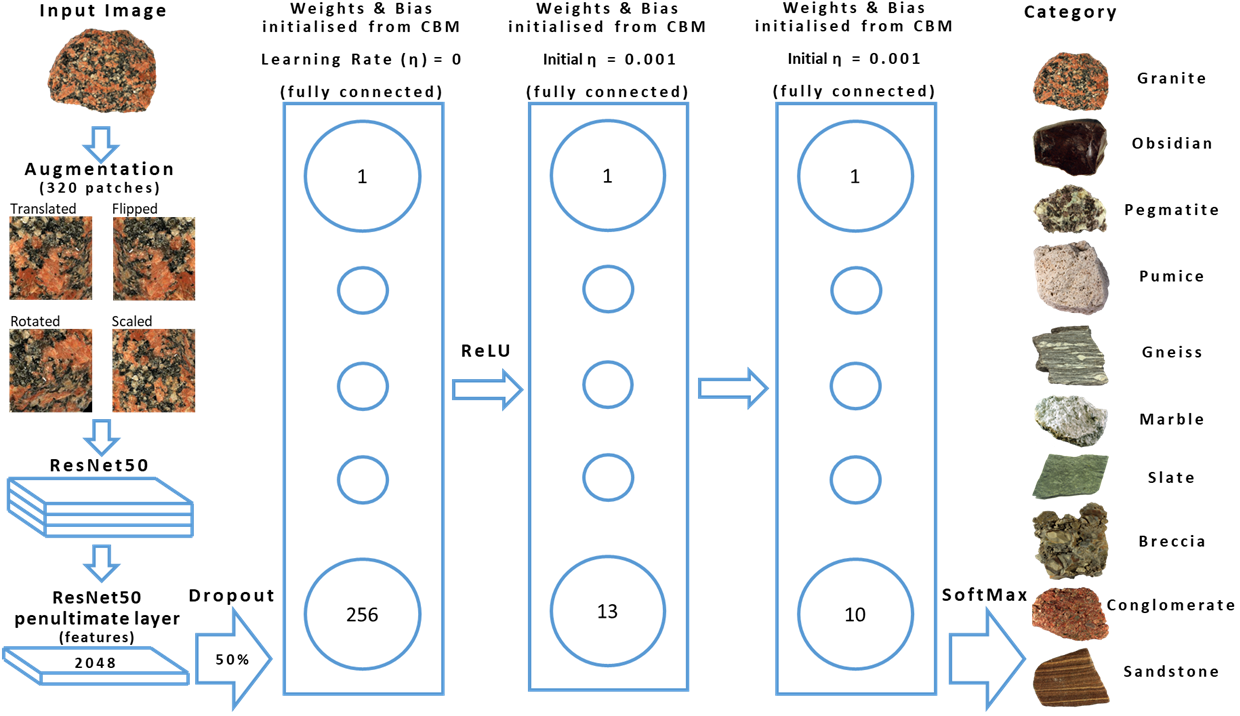
\includegraphics[width=\textwidth]{images/Hybrid Network Figure V2.png}
    \caption{The framework of the hybrid CBM classifier} \label{fig:Hybrid classifier XAI&I}
\end{figure}

Concurrently an partially feature constrained black-box model was developed akin to that in \cite{grangeXAISelfexplanatoryAI2022} (see figure \ref{fig:Networks 1-3 XAI&I}). The number of feature nodes was set to 13 in order to enable a a fair comparison to that of the hybrid CBM.

For one to achieve a sufficient set of data to equate to fair analysis of variance, the code was automated (see code ~\ref{lst:Automating 12 runs of 12 sets of validation images}) to complete 12 runs of 12 alternating validation sets. The output of each of which required collation and manipulation for analysis of accuracy, and concept alignment between each of the networks and that of the original set of expert ratings (an example of the training data used for Granite can be seen her \ref{An Example of 13 Expert Feature Ratings for Granite - As Used for Training})

Analysis of the immense collation of data from each permutation and manipulation of the models required the development of a plethora of Jupyter notebooks insights it held(\ref{fig:Code for the Analysis and Visualisation of Pearson's Correlation Co-Efficient of Feature Ratings Between Expert Feature Ratings, Sequential CBM and Hybrid Classifier CBM}, \ref{fig:Means and Standard Error of the Mean (SEM) Between Validation Sets - Analysis and Visualisation coded in Jupyter Notebooks using Plotly for Visualisation}, \ref{fig:Comparing the Accuracy of Rock Predictions - Hybrid - Continuous vs Binary Crystal Ratings}), with which manipulate the data and visualise it using the Python library \emph{Plotly} \cite{plotly} (see Appendix subsection: \ref{Data Visualisations}). This served as in order to expedite insight at a far greater pace.

\newpage
\section{Results}

My initial investigation took the form of manipulating training variables such as the number of epochs, mini-batch size and learning rate.

Through the analysis of training data visualisations it was clear that  validation accuracy of the original CBM was diverging from the training accuracy as I increased the number of epochs, a sign of the over-fitting the data. As such, the correlation of the output features with that of expert features was not negatively effected, with insignificant variance. The opposite was true when reducing the number of epochs, with a sweet spot between 175-200. As such, I decided to stick to the existing use of 200 epochs, as this made it simpler when comparing to previous iterations.

The manipulation of learning rate was of little benefit to the existing CBM model, reducing performance when the number of epochs was increased, yet was not significant enough to warrant further exploration. I believe this in part to be the benefit of the \emph{Adam Optimiser} \cite{Kingma2014Dec}, of which upon research appears to be a common effect due to its inherent ability to self-tune. Therefore I concluded that leave the learning rate at $10^{-3}$ (0.001) was adequate.

The manipulation of mini-batch size is another method typically used to prevent validation accuracy from diverging from training accuracy. I explored the use of reducing the size down to 256, which appeared to decrease divergence, however was of no benefit to performance. Upon further reading, many note that in some instance some over-fitting can be beneficial to a model, and as I was going to explore the benefits of appending the hybrid classifier, I returned to using a mini-batch size of 1024. 

For further analysis, some of the results of these manipulations can be seen in the appendix \ref{Feature Correlations - 13 Features - Continuous Scalar Crystal Rating 1 Run of 12 Alternating Validation Sets - Part 2}.

Despite there being no grand finding from the manipulation of training variables, the results from the use of the hybrid network were however successful, with the aim of achieving an improved accuracy in classification that is on par to that of a black-box model. The 13 feature hybrid CBM classifier achieved a classification accuracy of 87.8\% (SD 0.58\%), an improvement of 1.27\% in comparison to the partially feature-constrained model of 86.53\% (SD 4.39\%) and unconstrained network’s performance (mean 86.8\%, SD 0.8\%). Interestingly the 12 feature network, with the weakly correlated n the concept of \emph{Brightness Heterogeneity} removed (Continuous crystal rating CBM network \emph{r} = 0.43, Hybrid CBM network \emph{r} = 0.3, Binary crystal rating CBM network \emph{r} = 0.45, Hybrid CBM network \emph{r} = 0.27, \ref{Data Visualisations}) performed well achieving a higher classification accuracy mean of 88.36\% yet with a larger standard deviation of the means of 3.41\%.


\scriptsize
\begin{longtable}[c]{@{}llllll@{}}
 &
  \multicolumn{2}{c}{\textbf{13 Features}} &
  \multicolumn{1}{c}{\textbf{Unconstrained 13}} &
  \multicolumn{2}{c}{\textbf{12 Features}} \\
  \toprule
\endfirsthead
%
\multicolumn{6}{c}%
{{\bfseries Table \thetable\ continued from previous page}} \\
\endhead
%
 &
  \cellcolor[HTML]{E2EFDA}\textbf{Continuous} &
  \cellcolor[HTML]{FFE699}\textbf{Binary Crystal} &
  \cellcolor[HTML]{D9E1F2}\textbf{} &
  \cellcolor[HTML]{E2EFDA}\textbf{Continuous} &
  \cellcolor[HTML]{FFE699}\textbf{Binary Crystal} \\
  \toprule
\textbf{Runs/Val Sets} &
  \cellcolor[HTML]{FCE4D6}12/12 &
  \cellcolor[HTML]{FCE4D6}12/12 &
  \cellcolor[HTML]{FCE4D6}12/12 &
  \cellcolor[HTML]{FCE4D6}12/12 &
  \cellcolor[HTML]{FCE4D6}12/12 \\
  \toprule
\rowcolor[HTML]{E7E6E6} 
\textbf{C2} &
   &
   &
   &
   &
   \\
\textbf{Epochs} &
  \cellcolor[HTML]{E2EFDA}200 &
  \cellcolor[HTML]{FFE699}200 &
  \cellcolor[HTML]{D9E1F2}200 &
  \cellcolor[HTML]{E2EFDA}200 &
  \cellcolor[HTML]{FFE699}200 \\
\textbf{Learning Rate} &
  \cellcolor[HTML]{E2EFDA}{\color[HTML]{202124} 0.001} &
  \cellcolor[HTML]{FFE699}{\color[HTML]{202124} 0.001} &
  \cellcolor[HTML]{D9E1F2}{\color[HTML]{202124} 0.001} &
  \cellcolor[HTML]{E2EFDA}{\color[HTML]{202124} 0.001} &
  \cellcolor[HTML]{FFE699}{\color[HTML]{202124} 0.001} \\
\textbf{Learning Rate} &
  \cellcolor[HTML]{E2EFDA}{\color[HTML]{202124} 10\textasciicircum{}-3} &
  \cellcolor[HTML]{FFE699}{\color[HTML]{202124} 10\textasciicircum{}-3} &
  \cellcolor[HTML]{D9E1F2}{\color[HTML]{202124} 10\textasciicircum{}-3} &
  \cellcolor[HTML]{E2EFDA}{\color[HTML]{202124} 10\textasciicircum{}-3} &
  \cellcolor[HTML]{FFE699}{\color[HTML]{202124} 10\textasciicircum{}-3} \\
\textbf{Minibatch Size} &
  \cellcolor[HTML]{E2EFDA}{\color[HTML]{202124} 1024} &
  \cellcolor[HTML]{FFE699}{\color[HTML]{202124} 1024} &
  \cellcolor[HTML]{D9E1F2}{\color[HTML]{202124} 1024} &
  \cellcolor[HTML]{E2EFDA}{\color[HTML]{202124} 1024} &
  \cellcolor[HTML]{FFE699}{\color[HTML]{202124} 1024} \\
\textbf{Accuracy Mean - Val Set} &
  \cellcolor[HTML]{E2EFDA}83.66\% &
  \cellcolor[HTML]{FFE699}84.63\% &
  \cellcolor[HTML]{D9E1F2}\textbf{87.15\%} &
  \cellcolor[HTML]{E2EFDA}82.25\% &
  \cellcolor[HTML]{FFE699}82.48\% \\
\textbf{SEM - Val Set} &
  \cellcolor[HTML]{E2EFDA}0.52\% &
  \cellcolor[HTML]{FFE699}0.53\% &
  \cellcolor[HTML]{D9E1F2}0.83\% &
  \cellcolor[HTML]{E2EFDA}0.52\% &
  \cellcolor[HTML]{FFE699}0.57\% \\
\textbf{Accuracy Mean - Run Set} &
  \cellcolor[HTML]{E2EFDA}83.66\% &
  \cellcolor[HTML]{FFE699}84.63\% &
  \cellcolor[HTML]{D9E1F2}\textbf{86.53\%} &
  \cellcolor[HTML]{E2EFDA}82.25\% &
  \cellcolor[HTML]{FFE699}82.48\% \\
\textbf{STD of Means - Run Set} &
  \cellcolor[HTML]{E2EFDA}0.57\% &
  \cellcolor[HTML]{FFE699}\textbf{4.03\%} &
  \cellcolor[HTML]{D9E1F2}\textbf{4.39\%} &
  \cellcolor[HTML]{E2EFDA}\textbf{3.57\%} &
  \cellcolor[HTML]{FFE699}2.79\% \\
\textbf{SEM - Run Set} &
  \cellcolor[HTML]{E2EFDA}0.16\% &
  \cellcolor[HTML]{FFE699}1.16\% &
  \cellcolor[HTML]{D9E1F2}1.27\% &
  \cellcolor[HTML]{E2EFDA}1.03\% &
  \cellcolor[HTML]{FFE699}0.80\% \\
  \toprule
\rowcolor[HTML]{E7E6E6} 
\textbf{Hybrid} &
   &
   &
   &
   &
   \\
   
\textbf{Epochs} &
  \cellcolor[HTML]{E2EFDA}50 &
  \cellcolor[HTML]{FFE699}50 &
  \cellcolor[HTML]{D9E1F2} &
  \cellcolor[HTML]{E2EFDA}50 &
  \cellcolor[HTML]{FFE699}50 \\
\textbf{Learning Rate} &
  \cellcolor[HTML]{E2EFDA}{\color[HTML]{202124} 0.001} &
  \cellcolor[HTML]{FFE699}{\color[HTML]{202124} 0.001} &
  \cellcolor[HTML]{D9E1F2}{\color[HTML]{202124} } &
  \cellcolor[HTML]{E2EFDA}{\color[HTML]{202124} 0.001} &
  \cellcolor[HTML]{FFE699}{\color[HTML]{202124} 0.001} \\
\textbf{Learning Rate} &
  \cellcolor[HTML]{E2EFDA}{\color[HTML]{202124} 10\textasciicircum{}-3} &
  \cellcolor[HTML]{FFE699}{\color[HTML]{202124} 10\textasciicircum{}-3} &
  \cellcolor[HTML]{D9E1F2}{\color[HTML]{202124} } &
  \cellcolor[HTML]{E2EFDA}{\color[HTML]{202124} 10\textasciicircum{}-3} &
  \cellcolor[HTML]{FFE699}{\color[HTML]{202124} 10\textasciicircum{}-3} \\
\textbf{Minibatch Size} &
  \cellcolor[HTML]{E2EFDA}1024 &
  \cellcolor[HTML]{FFE699}1024 &
  \cellcolor[HTML]{D9E1F2} &
  \cellcolor[HTML]{E2EFDA}1024 &
  \cellcolor[HTML]{FFE699}1024 \\
\textbf{Accuracy Mean -  Val Set} &
  \cellcolor[HTML]{E2EFDA}87.80\% &
  \cellcolor[HTML]{FFE699}87.59\% &
  \cellcolor[HTML]{D9E1F2} &
  \cellcolor[HTML]{E2EFDA}87.55\% &
  \cellcolor[HTML]{FFE699}\textbf{88.36\%} \\
\textbf{SEM - Val Set} &
  \cellcolor[HTML]{E2EFDA}0.68\% &
  \cellcolor[HTML]{FFE699}0.70\% &
  \cellcolor[HTML]{D9E1F2} &
  \cellcolor[HTML]{E2EFDA}0.65\% &
  \cellcolor[HTML]{FFE699}\textbf{0.62\%} \\
\textbf{Accuracy Mean - Run Set} &
  \cellcolor[HTML]{E2EFDA}\textbf{87.80\%} &
  \cellcolor[HTML]{FFE699}87.59\% &
  \cellcolor[HTML]{D9E1F2} &
  \cellcolor[HTML]{E2EFDA}87.55\% &
  \cellcolor[HTML]{FFE699}\textbf{88.36\%} \\
\textbf{STD of Means - Run Set} &
  \cellcolor[HTML]{E2EFDA}0.58\% &
  \cellcolor[HTML]{FFE699}\textbf{2.94\%} &
  \cellcolor[HTML]{D9E1F2}\textbf{} &
  \cellcolor[HTML]{E2EFDA}3.43\% &
  \cellcolor[HTML]{FFE699}\textbf{3.41\%} \\
\textbf{SEM - Run Set} &
  \cellcolor[HTML]{E2EFDA}0.17\% &
  \cellcolor[HTML]{FFE699}0.85\% &
  \cellcolor[HTML]{D9E1F2} &
  \cellcolor[HTML]{E2EFDA}0.99\% &
  \cellcolor[HTML]{FFE699}0.98\%
  \\
\caption{Classification accuracy ratings comparing network variables. The first two columns use 13 expert feature ratings for training and compare implications of using continuous or binary ratings for the presence of crystals. The "13 Unconstrained" column represents a black-box model, limited only by the constraint of using a layer of 13 nodes prior to classification. The last two columns use 12 expert feature ratings, with the most weakly correlated feature "Brightness Heterogeneity" removed. A comparison is also drawn as to the implications of using continuous or binary ratings for the presence of crystals.}
\label{Classification accuracy ratings comparing network variables}\\
\end{longtable}

\normalsize
\chapter{Analysis}

To gain further insight as to what was happening with regards to the validity of the concepts I undertook some analysis of the importance of the weights, looking at L2 regularisation. The results below indicate towards a clearer lack of complexity for the network to understand the importance of feature concepts i.e. due to the hybrid network having lower weights (closer to 0) so prevents some over fitting is prevented perhaps. Further granular analysis of this scan be viewed in the appendix (\ref{Weights and calculated L2 regularisation values from a single run of a validation set (Images 1,2,3). Sequential CBM, 13 Features and binary rated crystals}.

\begin{table}[H]
\centering
\begin{tabular}{@{}lll@{}}
                      & \multicolumn{1}{c}{\cellcolor[HTML]{DDEBF7}\textbf{sCBM}} & \multicolumn{1}{c}{\cellcolor[HTML]{E2EFDA}\textbf{Hybrid}} \\
\textbf{All Concepts} & \multicolumn{1}{c}{\textbf{Sum L2}}                       & \multicolumn{1}{c}{\textbf{Sum L2}}                         \\
\rowcolor[HTML]{F2F2F2} 
\textbf{Granite}      & 6.0152  & 5.9691  \\
\textbf{Obsidian}     & 2.5668  & 1.5327  \\
\rowcolor[HTML]{F2F2F2} 
\textbf{Pegmatite}    & 14.0439 & 10.8745 \\
\textbf{Pumice}       & 12.7726 & 8.2170  \\
\rowcolor[HTML]{F2F2F2} 
\textbf{Gneiss}       & 12.2029 & 9.6233  \\
\textbf{Marble}       & 19.6444 & 15.0057 \\
\rowcolor[HTML]{F2F2F2} 
\textbf{Slate}        & 18.1869 & 12.0342 \\
\textbf{Breccia}      & 9.0980  & 7.0099  \\
\rowcolor[HTML]{F2F2F2} 
\textbf{Conglomerate} & 7.7457  & 6.1521  \\
\textbf{Sandstone}    & 11.0264 & 8.7511  \\
\rowcolor[HTML]{FFF2CC} 
\textbf{Total L2}     & \textbf{113.3028}                                         & \textbf{85.1696}                                           
\end{tabular}
\\
\caption{Analysing the complexity of concepts between the sequential CBM and Hybrid Classifier CBM using summed L2 values for all concepts.  Data from a single run of a validation set (Images 1,2,3)}
\end{table}
\chapter{Conclusions}

Upon completing my research and experimentation within the realm of self-explanatory AI, it has become self-evident that employing tools like concept bottleneck models have the potential to greatly contributes to the fostering trust in AI through the clarity and correlation of which they can convey human interpretable data. However, the use of the variety of XAI tools is without doubt very domain dependent. A key example of this is the critical domain of medical diagnosis and use of imaging for disease detection. As it stands the vast majority of AI tools used within the healthcare diagnosis domain come in the form of saliency maps \cite{holzingerXxAIExplainableAI2022a}. I believe that to truly foster trust and subsequently facilitate the use of AI for informed and improved decision making , multiple explanatory tools will be required, and tailored to the relevant stakeholders, be they medical doctors, lawmakers, data scientists or the public. The addition of explanatory data such as feature concept ratings from a model trained on “human in the loop”/expert data (self-explanatory, concept bottleneck etc.), the accuracy the model gives for its classification, as well as saliency maps (individually or collectively ) to reinforce what the model has detected. 

Yet one should be careful as to not overload the individual with too much information., as this may hinder decision making; say for example if the models don’t correlate with each other in diagnosis (feature concepts don’t correlate with saliency maps), or at the other end of the spectrum, the accuracy of the AI is so high that trust has bequeathed to an over reliance on AI tools resulting in misdiagnosis. The combination of methods is perhaps one way in which to combat over reliance, as referencing will always require a human in the loop, and as previously alluded to, if models do not correlate multiple experts may be required to communicate as the their interpretation with individual expert knowledge. 

To include a broader range of categorisations (in the domain of rocks), one would presume that additional nodes and concepts may have to added to distinguish the finite differences between rocks of similar appearance visually. The challenge of a humans ability to distinguishing one rock type from another was highlighted by Nosofsky \cite{nosofskyLearningNaturalScienceCategories2017} using MDS co-ordinates, 

Despite the improvements in performance by the hybrid classifier network, there were still some instances where by the sequential CBM outperformed, possibly due to the quality of the image or the ratings data itself: "all dataset-based methods are limited by the diversity of examples in the dataset used and the quality of labels." \cite{raukerTransparentAISurvey2023}. The unpicking of this unfortunately evaded my capabilities in the time available.

Instances where C2 outperformed Hybrid
\begin{itemize}
    \item 13 Features \& Binary Crystal Rating 
        \begin{itemize}
        \item Val 3, 6, 12 = C2 (mean = 83.61\%, SEM = 0.27\%), Hybrid (mean = 83.1\%, SEM = 0.92\%)
        \item Val 2, 7, 10 = C2 (mean = 87.78\%, SEM = 0.72\%), Hybrid (mean = 85.56\%, SEM = 0.60\%)
        \end{itemize}
            \begin{figure}[H]
            \centering
            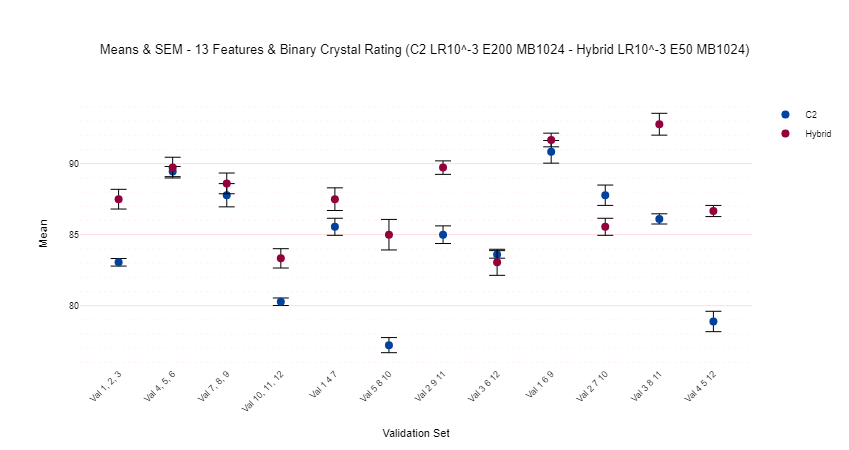
\includegraphics[width=0.8\textwidth]{images/Means & SEM - 13 Features & Binary Crystal Rating (C2 LR10^-3 E200 MB1024 - Hybrid LR10^-3 E50 MB1024).png}
            \end{figure}
        \vspace{0.5cm}
    \item 13 Features \& Continuous Crystal Rating
        \begin{itemize}
        \item Val 2, 7, 10 = C2 (mean = 90.0\%, SEM = 0.79\%), Hybrid (mean = 86.39\%, SEM = 0.73\%)
        \end{itemize}
            \begin{figure}[H]
            \centering
            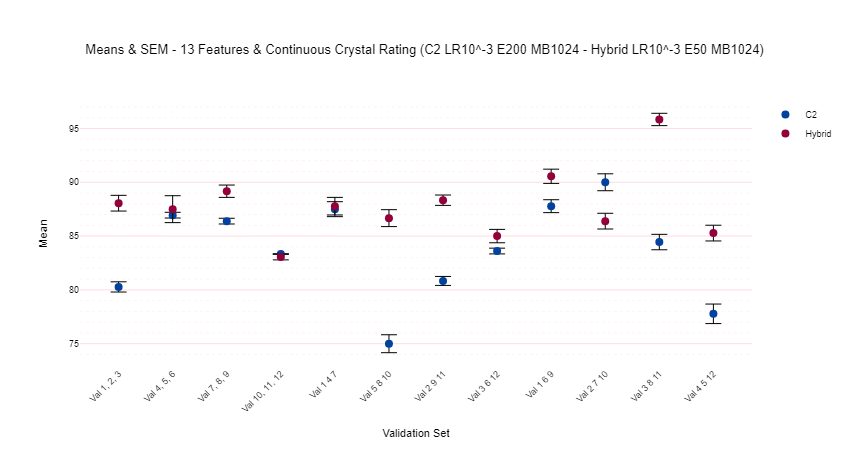
\includegraphics[width=0.8\textwidth]{images/Means & SEM - 13 Features & Continuous Crystal Rating (C2 LR10^-3 E200 MB1024 - Hybrid LR10^-3 E50 MB1024).png}
            \end{figure}
        \vspace{0.5cm}
    \item 12 Features \& Binary Crystal Rating 
        \begin{itemize}
        \item Val 1, 6, 9 = C2 (mean = 89.72\%, SEM = 0.47\%), Hybrid (mean = 89.17\%, SEM = 0.57\%)
        \end{itemize}
            \begin{figure}[H]
            \centering
            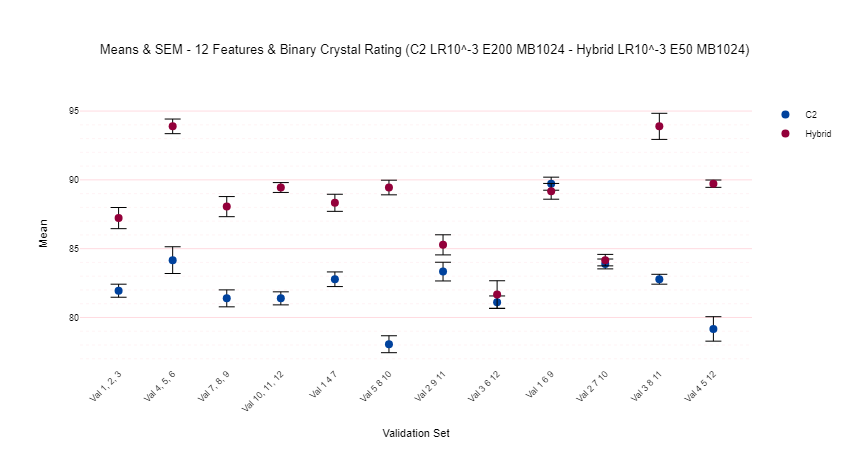
\includegraphics[width=0.8\textwidth]{images/Means & SEM - 12 Features & Binary Crystal Rating (C2 LR10^-3 E200 MB1024 - Hybrid LR10^-3 E50 MB1024).png}
            \end{figure}
        \vspace{0.5cm}
    \item 12 Features \& Continuous Crystal Rating
        \begin{itemize}
        \item Val 3, 6, 12 = C2 (mean = 83.33\%, SEM = 0.39\%), Hybrid (mean = 80.28\%, SEM = 0.83\%)
        \item Val 1, 6, 9 = C2 (mean = 87.50\%, SEM = 0.57\%), Hybrid (mean = 86.67\%, SEM = 0.88\%)
        \end{itemize}
            \begin{figure}[H]
            \centering
            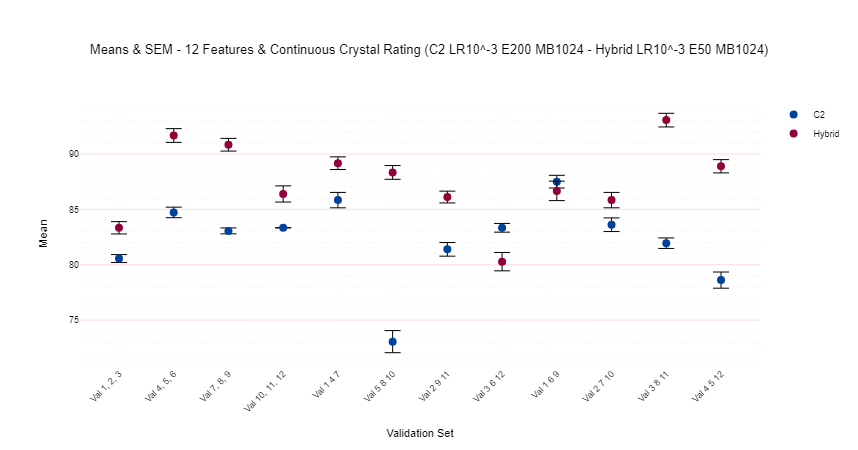
\includegraphics[width=0.8\textwidth]{images/Means & SEM - 12 Features & Continuous Crystal Rating (C2 LR10^-3 E200 MB1024 - Hybrid LR10^-3 E50 MB1024).png}
            \end{figure}
        \vspace{0.5cm}
\end{itemize}
\vspace{0.5cm}

In hindsight I would have have attempted to incorporate ConceptShAP \cite{yehCompletenessawareConceptBasedExplanations2019}, or another method for assessment of concept evaluation.

The increased use case for LLMs is of great intrigue, particularly with the development of multi-modal models, however this will require a far deeper dive by XAI researchers if the outputs are to be worth of trust.

\chapter{Reflection and Learning}

At the outset, the undertaking of this project was quite daunting, partially due to its inherent complexity, tackling a topic far beyond the technical scope of any of the taught modules covered in the MSc. I was therefore acutely aware that I was to be challenging myself considerably, both technically and academically, requiring me to learn at pace to deliver on my research aims.

The process of delivering this project has given me valuable insight into the breadth of skills required to deliver a program of research. It very quickly became apparent that time management and organisation skills were essential, along with the ability to be agile with ones aims and objectives. 

The use of a Gantt chart was helpful in enabling a broad overview of progress. However, I quickly discovered that when embarking on a novel research area that is inherently complexed and challenging to both one’s technical skills and domain knowledge, the intricacies of the tasks can require altering priorities at short notice. For example, running the required volume of iterations of the network could take anywhere between 2-3 days depending on how many permutations and training variables were altered. If a bug appeared in the the code, particularly one that I was not aware of due to the use of a remote machine, my workflow would have to pivot to allowing time for debugging. This made planning unwieldy at times, as each collation of results required data analysis from which I used to inform on the next permutations of the networks. 

In an ideal world the data analysis tools and skills to monitor the CNNs output would be a prerequisite before commencing with the research. However, the bespoke data analysis tools required for the task were not available from the outset, as I was not yet equipped with the skills and agility required to build them. As such, it initially took substantial time to complete analysis, using a combination of excel and Jupyter Notebooks, before fully transitioning to the latter. This limitation in my skill set served as a vital learning curve, as the desire to complete analysis at pace, drove me to learn a host of new skills in data manipulation. The acquisition of these new analysis skills, particularly in the visual format, served to reinforce my knowledge of data visualisation acquired during the taught phase of the MSc. The subsequent understanding from these visual aids made me vastly more agile, enabling me to hypothesise on the implications of my network alterations, and to re-aligning my objectives to fit within the limited time frame of the project. 

Initially the ambiguity of the time frames required for the network to run and the data to be analysed often meant that I found myself neglecting the Gantt chart and using a combination of handwritten notes and task lists, word documents comprised of hypotheses, and technical summaries, windows notepads for reminders of which permutation of the model was running on the remote machine, alongside a host of annotations in the code. As the whole process of data collection, analysis, literature acquisition and review became more fluid, I found myself returning to  the Gantt chart as means of keeping on top of progress.
In hindsight, I vastly overestimated my ability to complete the scale of research that I desired in such a short time frame. The discovery midway through the project that the manipulation of training options was not necessarily the best means to achieve increased accuracy, at least in this instance, redefined the scope of the project. Subsequently I made the executive decision to pivot my attention to analysing the effect of removing a weakly correlated feature concept and of altering concepts ratings as binary or scalar. Prior knowledge of neural network optimisation methods before undertaking this project would have saved a great deal of time and effort, however I learned a great deal in the process. I am now considerably more informed and skilled as making alterations to the inner working of CNNs and AI systems in general, of which I hope to apply in my work beyond this project. 

At the start of the project I was only briefly acquainted with Matlab, having used it for assisting co-workers in research activities. The subsequent development of the project in Matlab gave me a far greater understanding of the language and environment for the undertaking of research and development work. Despite this, it did hinder my ability to experiment with new methodologies and tools discovered in my literature search, of which the majority were typically developed in Python (and freely available on GitHub). Given the time and the opportunity I would preferred to have re-written the project in Python, and to have incorporated a means of using Shapley values \cite{yehCompletenessawareConceptBasedExplanations2019} to assess the model’s dependence on a concept/feature.

Due to my involvement in the conference paper \cite{grangeXAISelfexplanatoryAI2022} that inspired this dissertation, I was put in good stead to further embark on a wider literature review, to inform the necessity and relevancy of my work within the academic landscape. My thirst for knowledge and enthusiasm for discovering new methods and ideas in XAI put my time management skills to the test when undertaking the acquisition of literature for review. Upon reflection, I believe that my compulsion to understand the broader narrative as well as the granular, was essential, as it became apparent from reading the vast platitude of papers published on AI and XAI, that few in the field fully consider the inherent interdisciplinary nature of their work and the broader landscape in which it is sited e.g. psychology and philosophy.

The discovery of papers on covering self-explanatory or interpretable XAI models and methods that were conceptually relevant was a complexed task. The terminology used by authors is frequently used interchangeably, with multiple interpretations of their meanings thus posing a great challenge when making comparative evaluations of models. As such I decided to include a subsection within this dissertation addressing the issue, which not only aided my understanding, but hopefully the readers too.

The lack of commonly used methodologies by which to assess XAI approaches empirically was also preventative in assessing XAI models on any common ground. The field of Human Factors, HCI and Robotics have many tools at their disposal with which to use for empirical research, however those in XAI often appended their own methods for assessing the credibility of their work.  I sincerely hope that this will soon change with the very recent publication of papers addressing the issue (\cite{hoffmanMeasuresExplainableAI2023}, \cite{uenoTrustHumanAIInteraction2022}, \cite{perrigTrustIssuesTrust2023}, \cite{kleinMinimumNecessaryRigor2023}).

As my literature review was ongoing throughout the project, with my task of developing the hybrid sequential network already set out at the beginning of the project, it was near impossible to back track and incorporate any of the new tools that I subsequently discovered in the literature. The discovery of Koh et al.’s \cite{kohConceptBottleneckModels2020} paper was somewhat disheartening, with the proposal of a sequential CBM vastly akin to that proposed by Grange et al. \cite{grangeXAISelfexplanatoryAI2022}. However the lack of grounding in the psychological domain i.e. the research conducted by Nosofsky et al. set’s the papers apart significantly. The discovery Koh et al.’s paper did however inform me of the term “Concept Bottleneck Network”, of which greatly assisted my literature search due its adoption by subsequent researchers.

As such, the project has up-skilled me immensely, with an insight and knowledge to build my own tools and tackle debates over the preference of one methodology over another.

Throughout the project I lacked the benefit of garnering any insight for external experts (except at its inception) or empirical evidence with which to evaluate the validity of my models output e.g. conferring with geologists over the concepts used or measuring the skills of geologists to correctly classify the rocks by image alone (typically done by a variety of physical methods rather than visual alone). 

lessons about the topics addressed in the project where not already covered by the substance of your dissertation (underpinning theory or philosophy; value of approaches; understanding gained; problems not solved; effectiveness; etc.). 
\chapter{Appendix}

\section{Code Examples}

\subsection{Matlab code for the Hybrid Network Classifier}
\lstinputlisting[language=Matlab,firstline=559, lastline=605, caption= Matlab code for the Hybrid Network Classifier, label={lst:Matlab code for the Hybrid Network Classifier}]{Code/networksAll.m}

\subsection{Automating 12 runs of 12 sets of validation images}
\lstinputlisting[language=Matlab, caption= Matlab code for automating 12 runs of 12 sets of validation images, label={lst:Automating 12 runs of 12 sets of validation images}]{Code/automatedTwelveRuns.m}

\subsection{Analysis and Visualisation of Feature Ratings Correlation}
\begin{figure}[H]
  \centering
    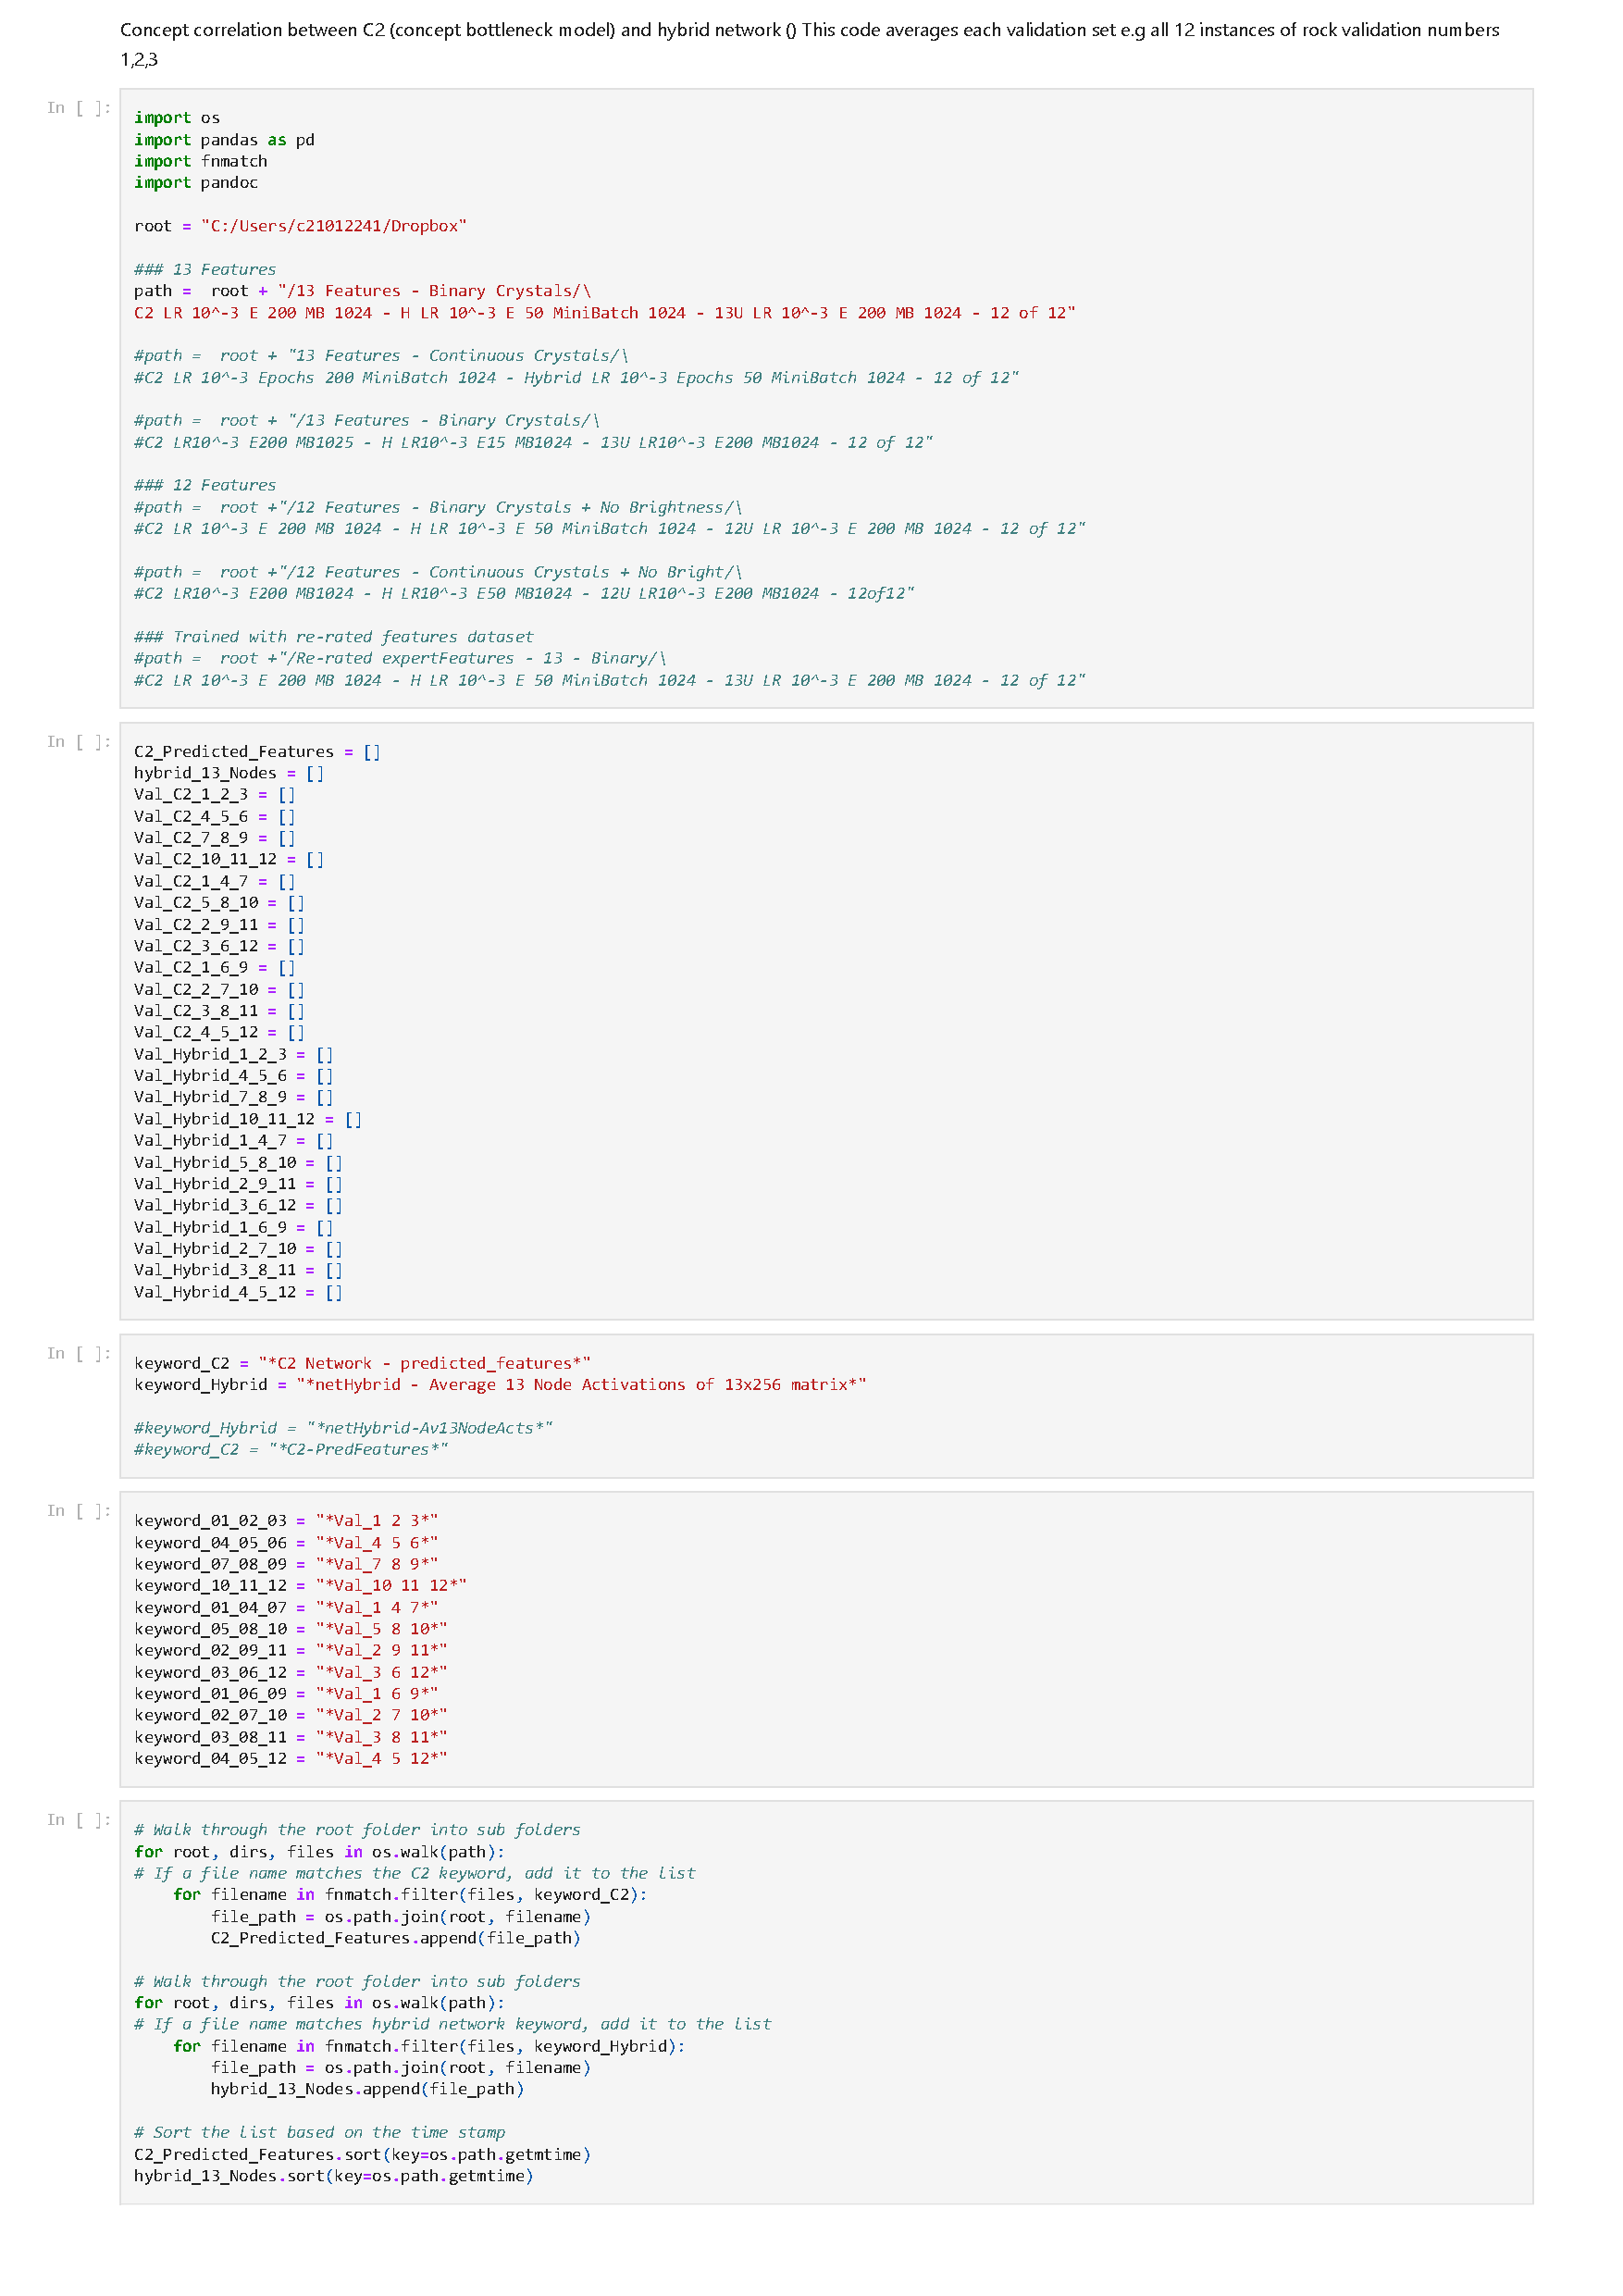
\includegraphics[width=0.92\textwidth, height=0.92\textheight]{Code/Correlation_Visualisation_and_CSV_for_Average_Feature_Ratings_-_12_of_12.pdf}
  \label{fig:Correlation Visualisation for Average Feature Ratings}
\end{figure}
\includepdf[pages=2-6, width=0.92\textwidth, height=0.92\textheight]{Code/Correlation_Visualisation_and_CSV_for_Average_Feature_Ratings_-_12_of_12.pdf}
\begin{figure}[H]
  \centering
    \includegraphics[page=7, width=0.92\textwidth, trim= 20 500 20 0, clip]{Code/Correlation_Visualisation_and_CSV_for_Average_Feature_Ratings_-_12_of_12.pdf}
    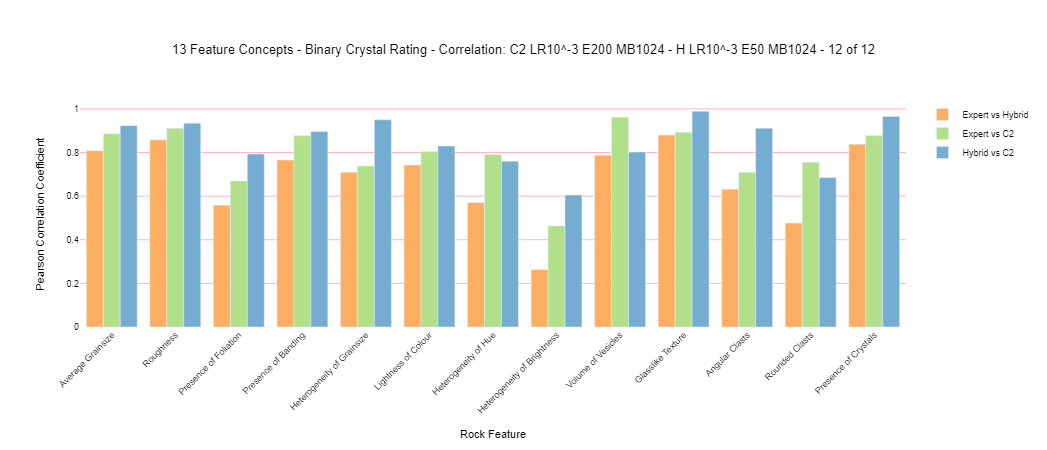
\includegraphics[width=0.92\textwidth, trim = 1cm 0.2cm 0.5cm 0, clip]{images/13 Feature Concepts - Binary Crystal Rating - Correlation- C2 LR10^-3 E200 MB1024 - H LR10^-3 E50 MB1024 - 12 of 12.png}
    \caption{Code for the Analysis and Visualisation of Pearson's Correlation Co-Efficient of Feature Ratings Between Expert Feature Ratings, Sequential CBM and Hybrid Classifier CBM. This was coded using Python in a Jupyter Notebook, and Plotly for visualisation} \label{fig:Code for the Analysis and Visualisation of Pearson's Correlation Co-Efficient of Feature Ratings Between Expert Feature Ratings, Sequential CBM and Hybrid Classifier CBM}
\end{figure}

\subsection{Means and Standard Error of the Mean (SEM) - Analysis and Visualisation using Plotly}
\begin{figure}[H]
  \centering
    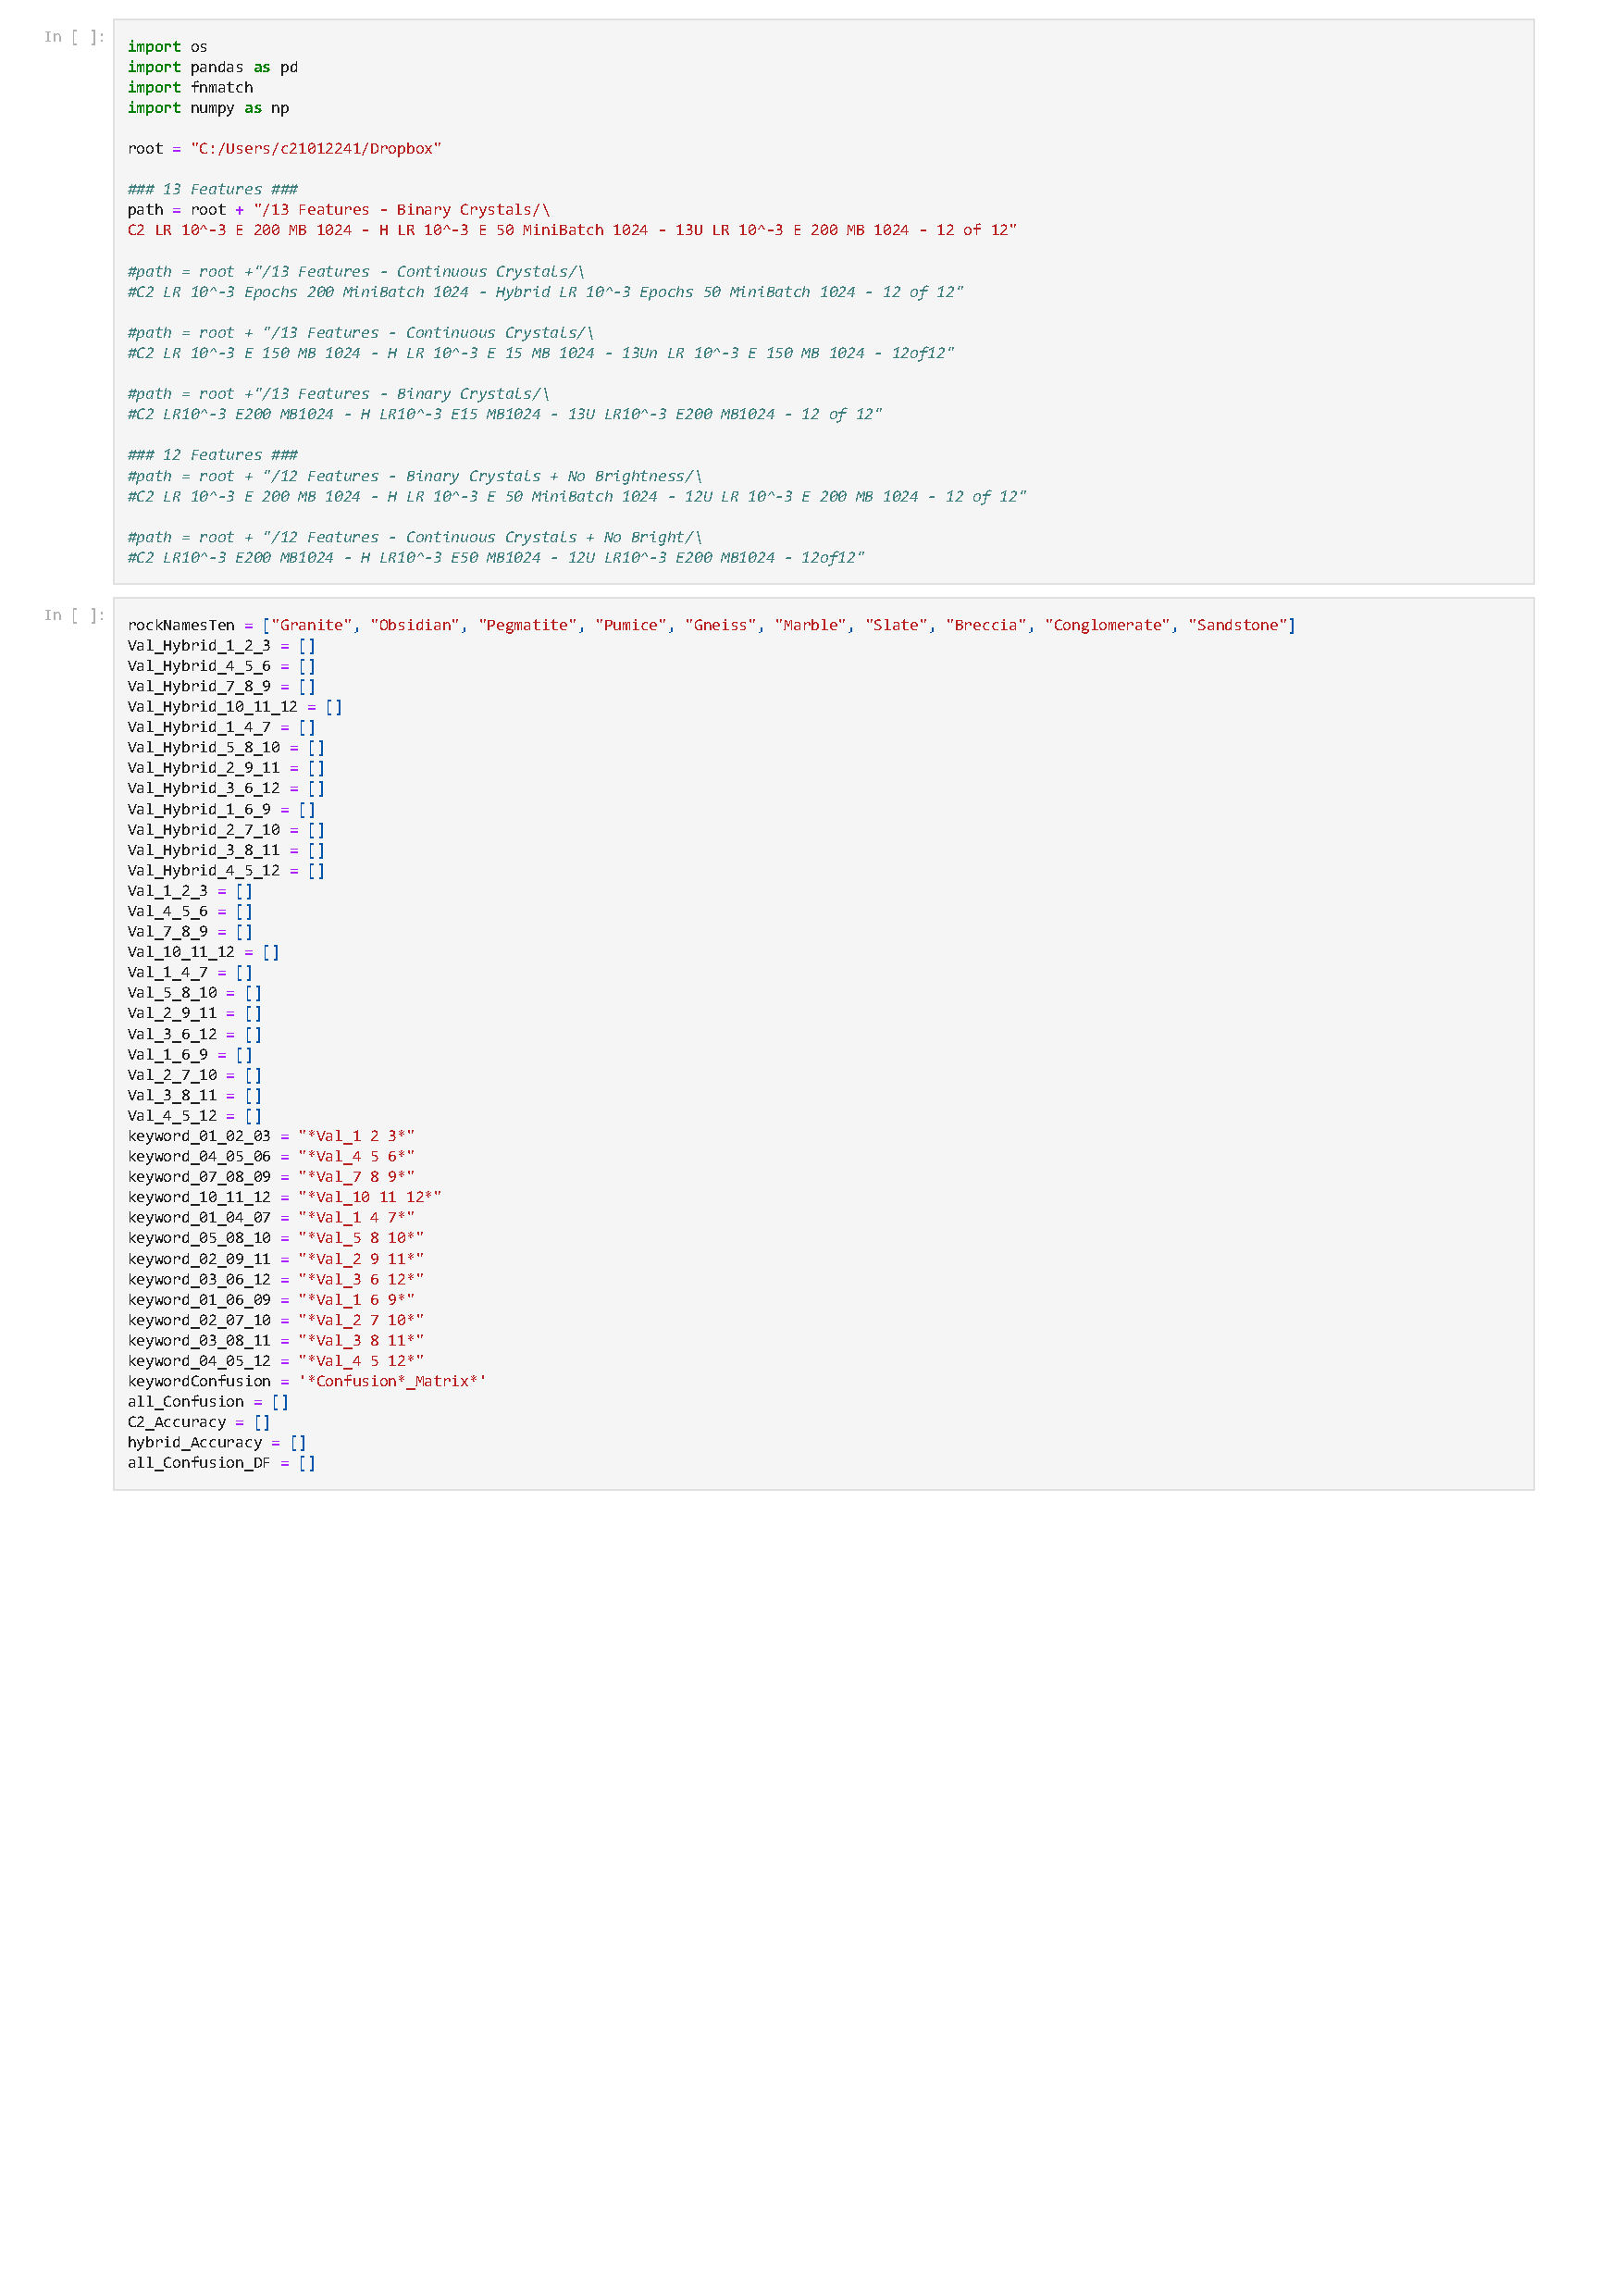
\includegraphics[width=0.99\textwidth, height=0.99\textheight]{Code/Mean_and_SEM_-_Visualisation_of_12_of_12_Validation_Sets.pdf}
  \label{fig:Mean_and_SEM_-_Visualisation_of_12_of_12_Validation_Sets}
\end{figure}
\includepdf[pages=2-6, width=0.99\textwidth, height=0.99\textheight]{Code/Mean_and_SEM_-_Visualisation_of_12_of_12_Validation_Sets.pdf}
\begin{figure}[H]
  \centering
    \includegraphics[page=7, width=0.95\textwidth, trim= 20 450 20 10, clip]{Code/Mean_and_SEM_-_Visualisation_of_12_of_12_Validation_Sets.pdf}
    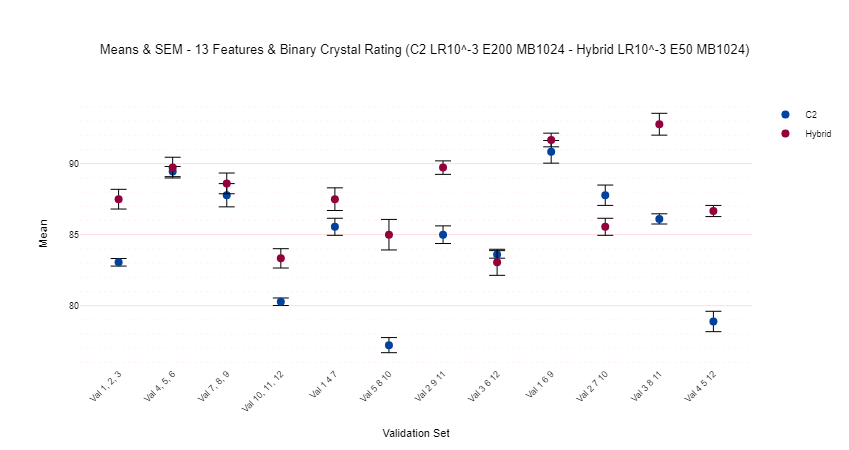
\includegraphics[width=0.85\textwidth, trim = 0.5cm 0cm 0.5cm 3.5cm, clip]{images/Means & SEM - 13 Features & Binary Crystal Rating (C2 LR10^-3 E200 MB1024 - Hybrid LR10^-3 E50 MB1024).png}
    \caption{Means and Standard Error of the Mean (SEM) Between Validation Sets - Analysis and Visualisation coded in Jupyter Notebooks using Plotly for Visualisation} \label{fig:Means and Standard Error of the Mean (SEM) Between Validation Sets - Analysis and Visualisation coded in Jupyter Notebooks using Plotly for Visualisation}
\end{figure}

% trim=left bottom right top

\subsection{Comparing the Accuracy of Rock Predictions - Hybrid - Continuous vs Binary Crystal Ratings}
\begin{figure}[H]
  \centering
    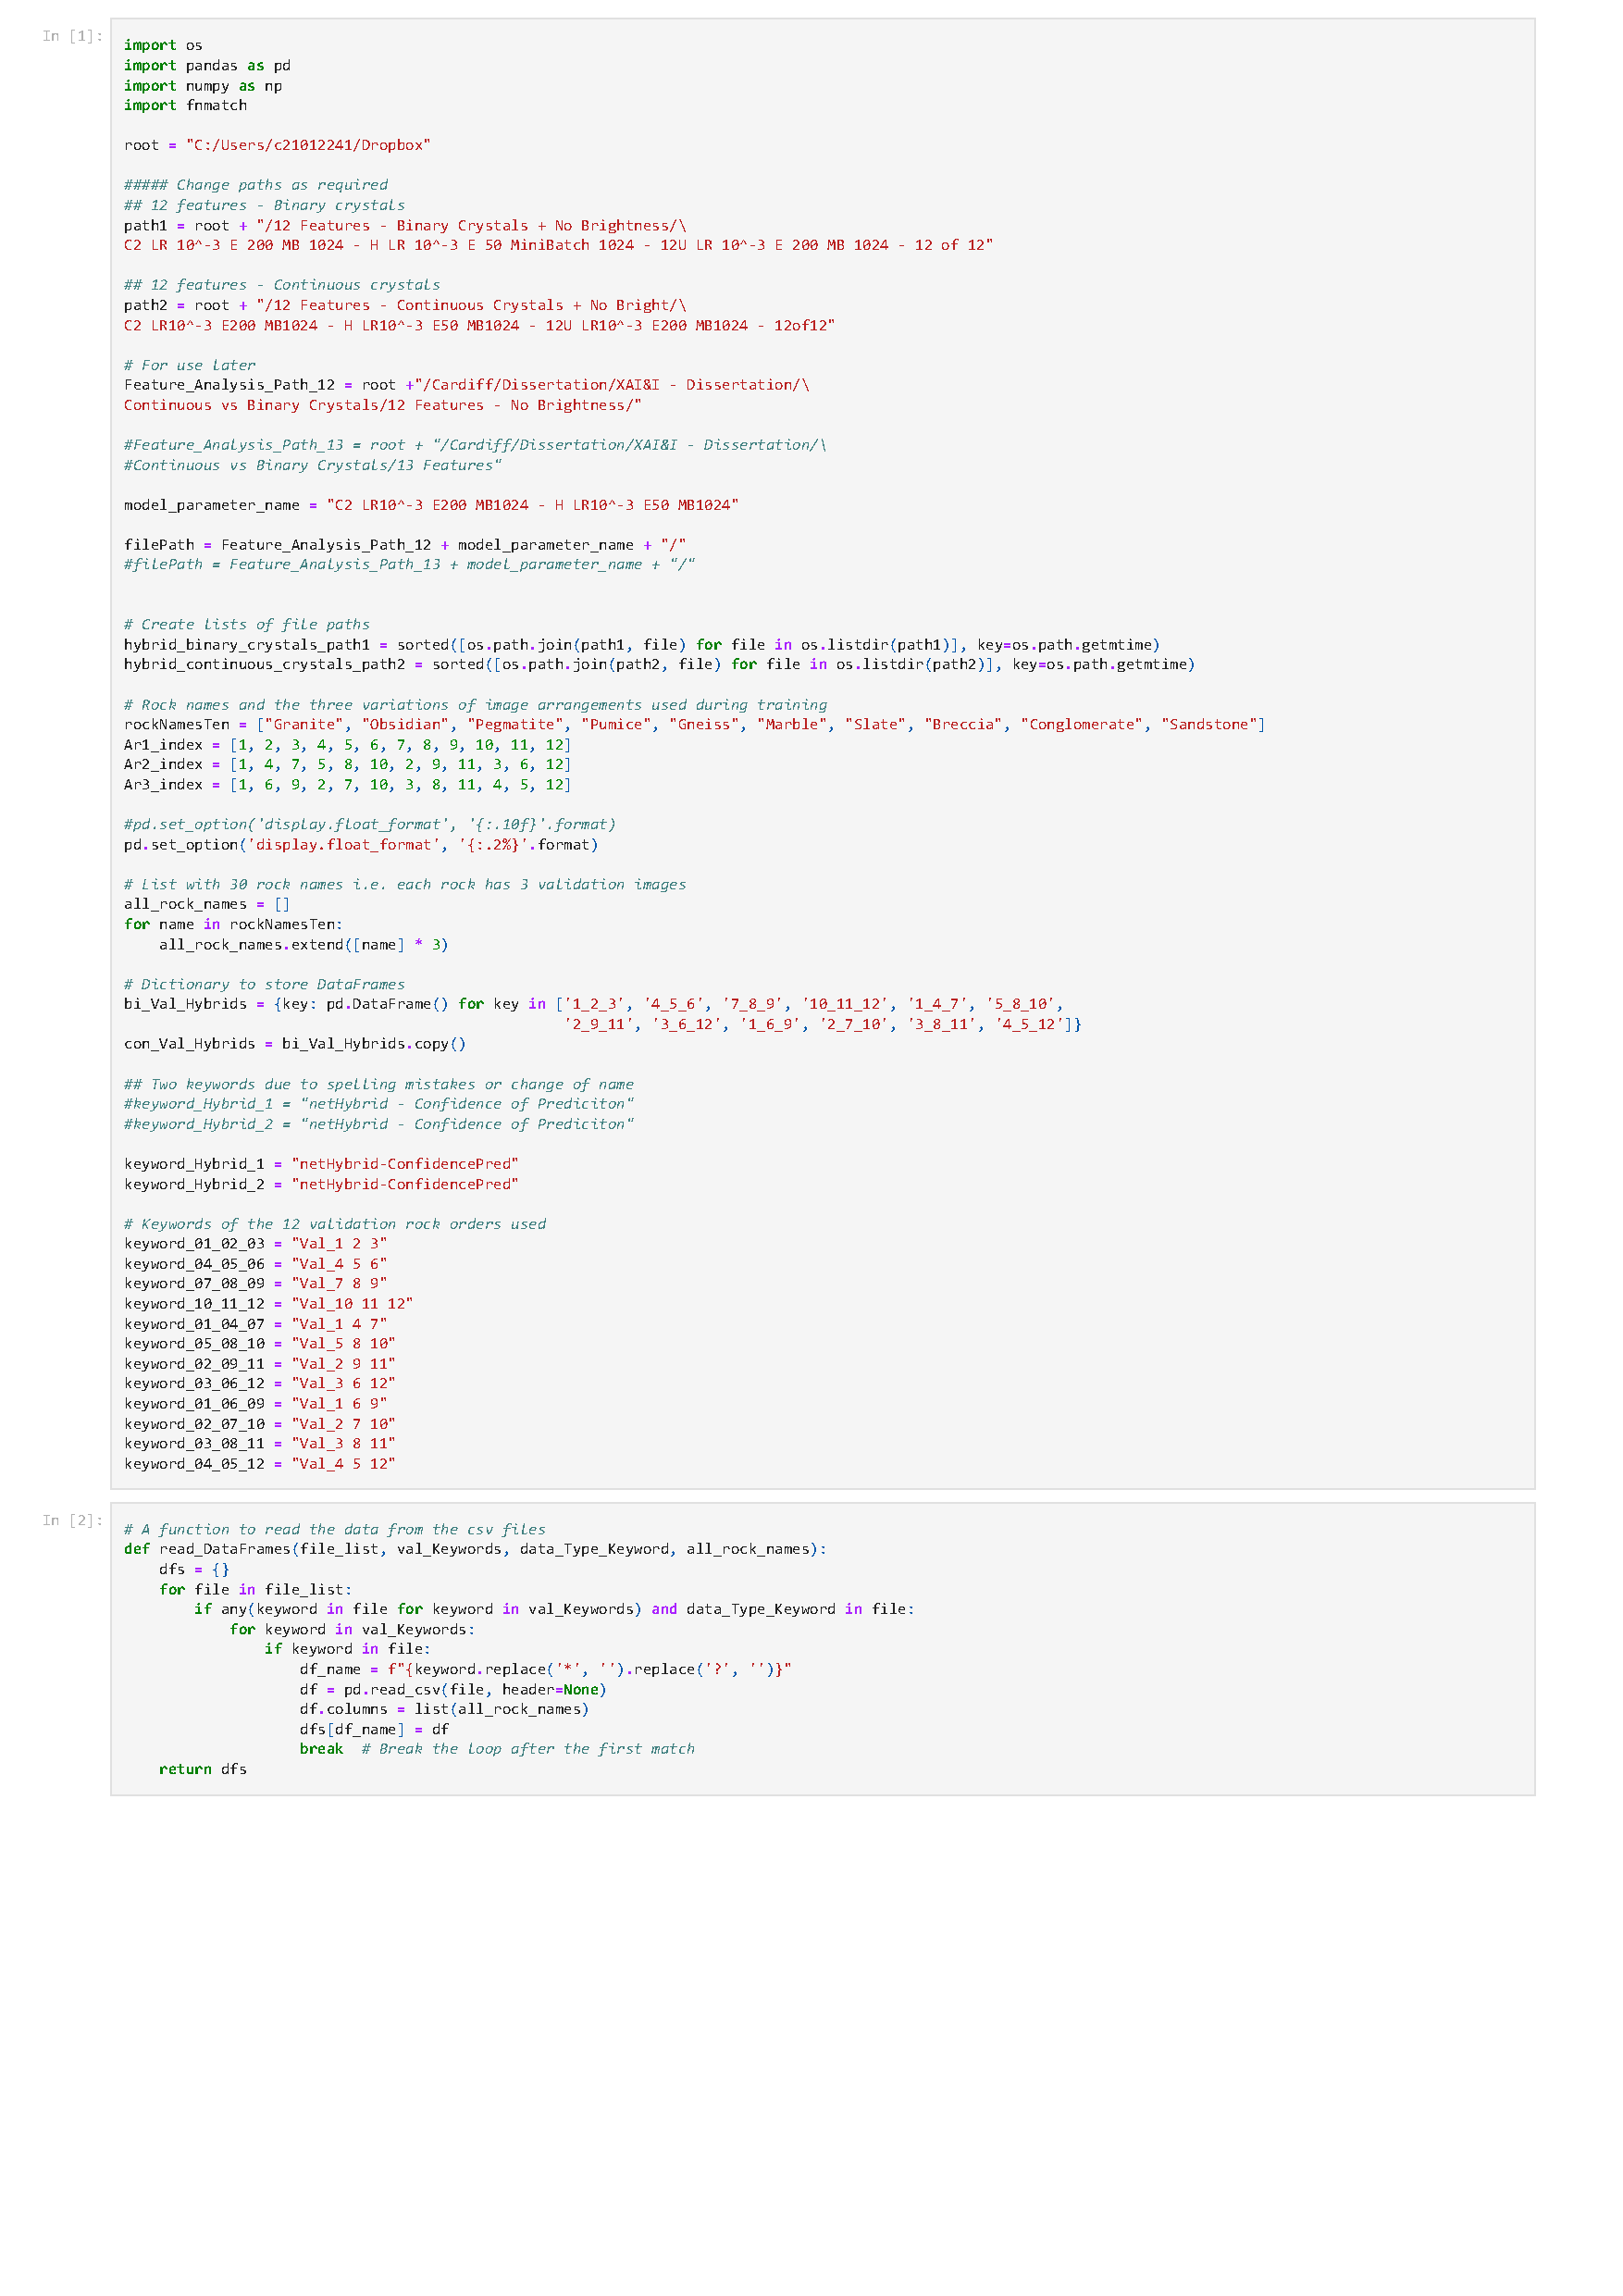
\includegraphics[width=0.9\textwidth, height=0.9\textheight]{Code/Compare2HybridModels V7.pdf}
\end{figure}
\includepdf[pages=2-5, width=0.9\textwidth, height=0.9\textheight]{Code/Compare2HybridModels V7.pdf}
%\includepdf[pages=6, width=0.9\textwidth, height=0.9\textheight, pagecommand={\null\vfill\captionof{lstlisting}{Comparing the Accuracy of Rock Predictions - Hybrid - Continuous vs Binary Crystal Ratings}}]{Code/Compare2HybridModels V7.pdf}
\begin{figure}[H]
  \centering
    \includegraphics[page=6, width=0.85\textwidth, trim= 20 100 20 10, clip]{Code/Compare2HybridModels V7.pdf}
    \caption{Comparing the Accuracy of Rock Predictions - Hybrid - Continuous vs Binary Crystal Ratings} \label{fig:Comparing the Accuracy of Rock Predictions - Hybrid - Continuous vs Binary Crystal Ratings}
\end{figure}



\section{Data Visualisations} \label{Data Visualisations}

\subsection{13 Features - Binary Crystal Rating} 

\begin{figure}[H]
  \centering
    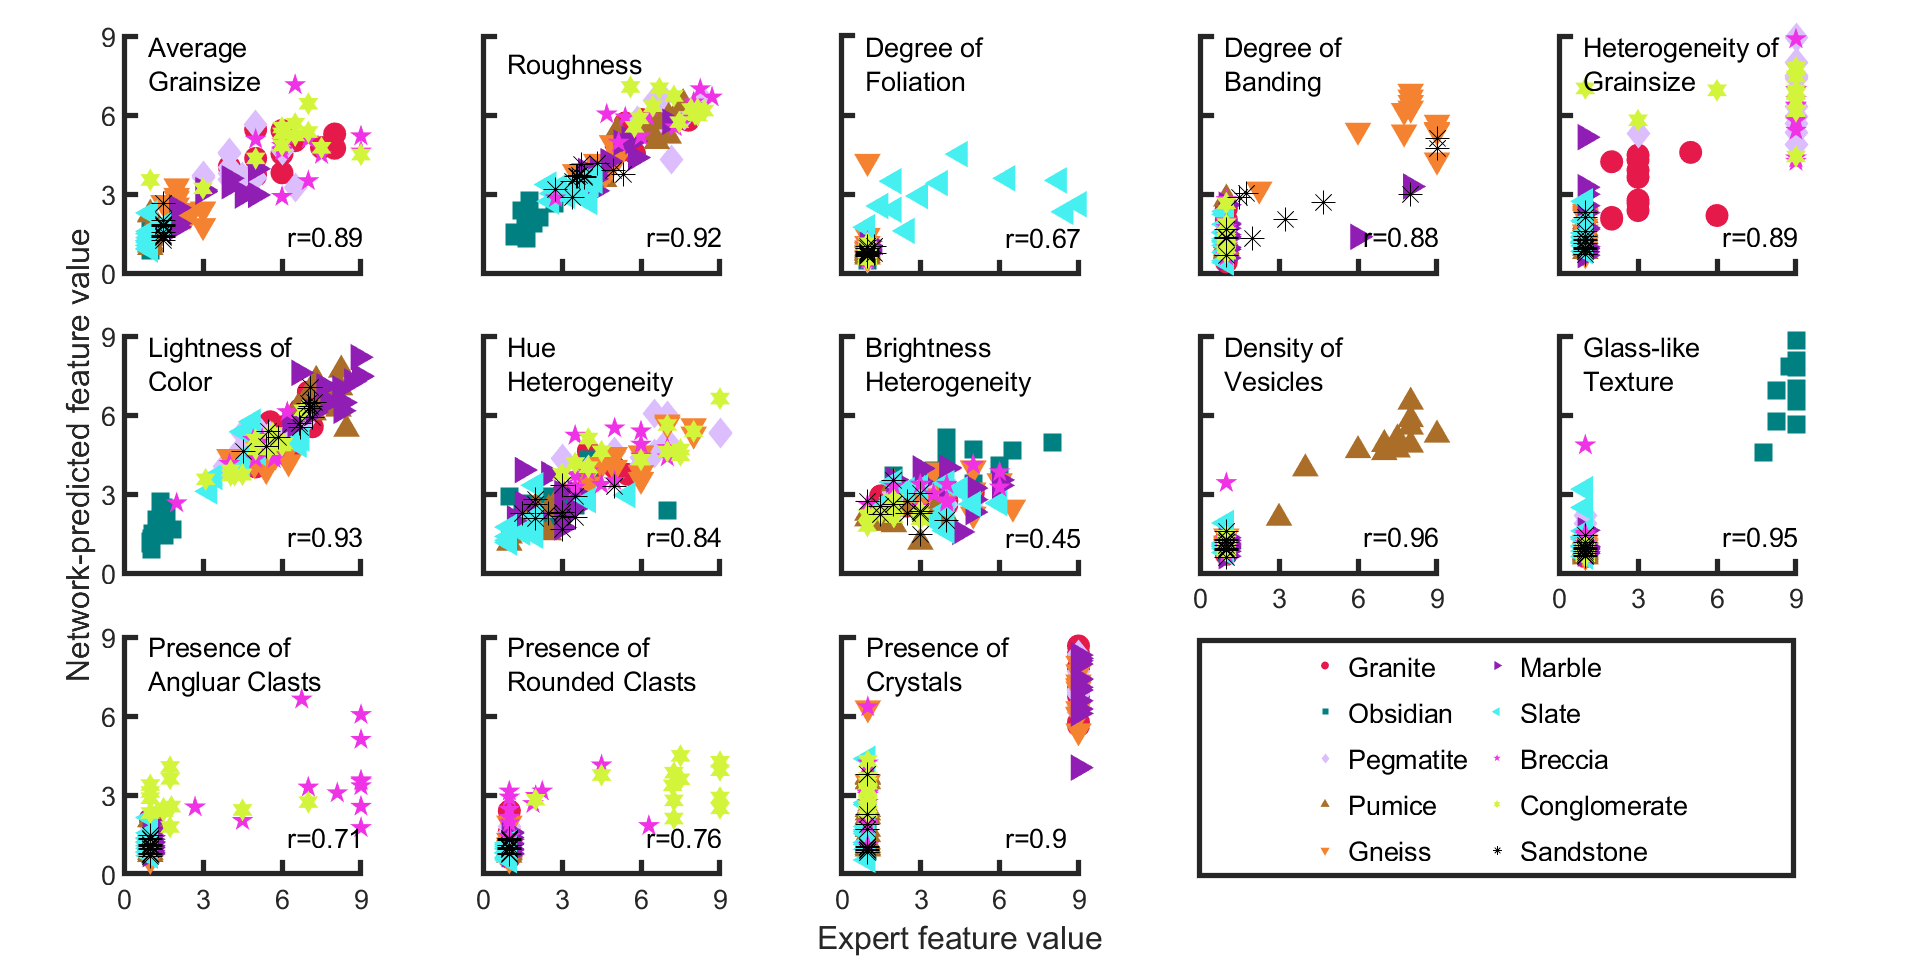
\includegraphics[width=\textwidth]{images/MATLAB Correlation - C2_Vs_Expert - 13 Feautres - Binary.png}
    \caption{Feature Correlation - Sequential CBM Vs Expert Ratings - 13 Features - Binary Crystal Rating} \label{fig:Feature Correlation - Sequential CBM Vs Expert Ratings - 13 Features - Binary Crystal Rating}
\end{figure}

\begin{figure}[H]
  \centering
    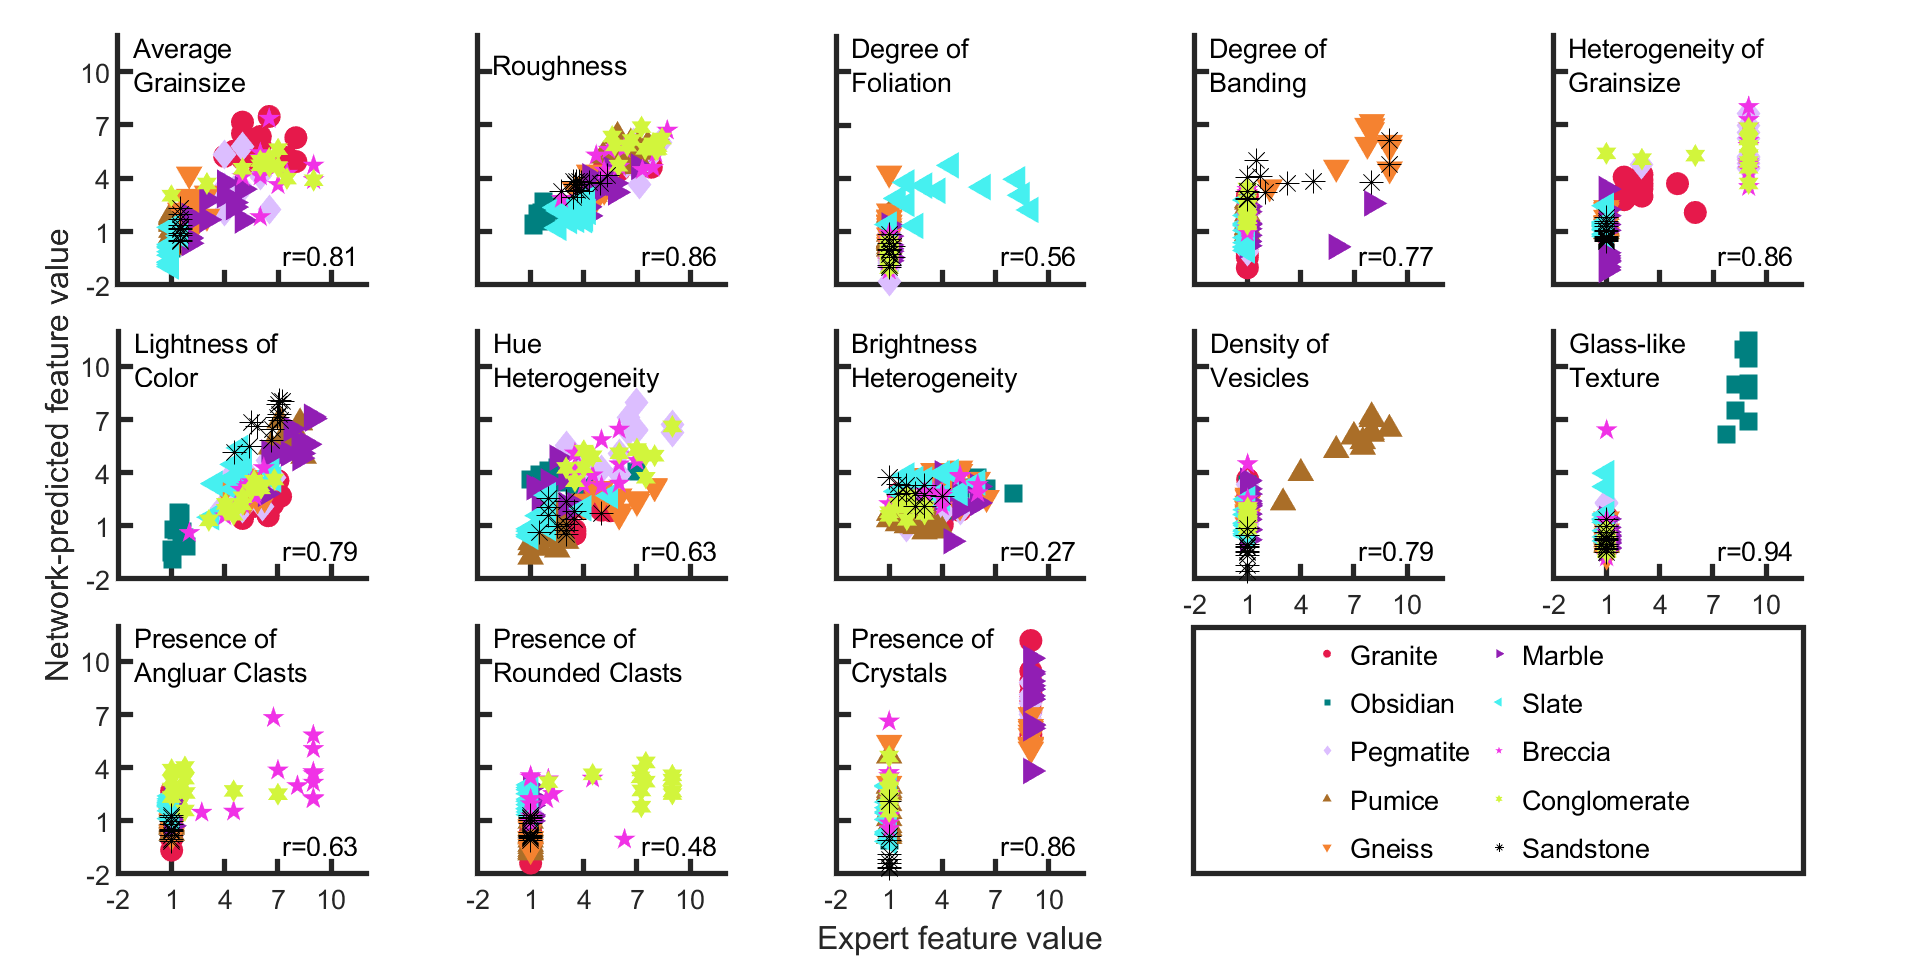
\includegraphics[width=\textwidth]{images/MATLAB Correlation - Hybrid_Vs_Expert - 13 Feautres - Binary.png}
    \caption{Feature Correlation - Hybrid Sequential CBM Vs Expert Ratings - 13 Features - Binary Crystal Rating} \label{fig:Feature Correlation - Hybrid Sequential CBM Vs Expert Ratings - 13 Features - Binary Crystal Rating}
\end{figure}

\begin{figure}[H]
  \centering
    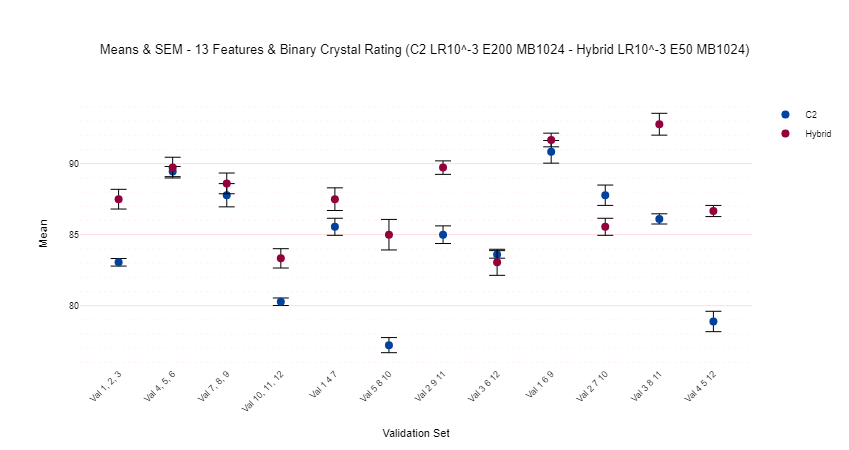
\includegraphics[width=\textwidth]{images/Means & SEM - 13 Features & Binary Crystal Rating (C2 LR10^-3 E200 MB1024 - Hybrid LR10^-3 E50 MB1024).png}
    \caption{Means \& SEM - Validation Sets - 13 Features - Binary Crystal Rating} \label{fig:Means & SEM - Validation Sets - 13 Features - Binary Crystal Rating}
\end{figure}


\begin{figure}[H]
  \centering
    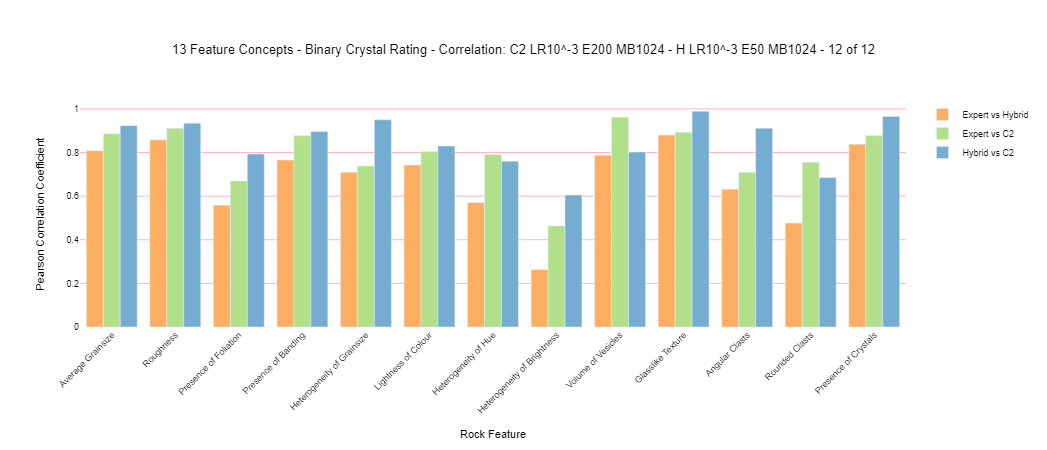
\includegraphics[width=\textwidth]{images/13 Feature Concepts - Binary Crystal Rating - Correlation- C2 LR10^-3 E200 MB1024 - H LR10^-3 E50 MB1024 - 12 of 12.png}
    \caption{13 Feature Concepts - Binary Crystal Rating - Mean correlation of Feature Concepts} \label{fig:13 Feature Concepts - Binary Crystal Rating - Mean correlation of Feature Concepts}
\end{figure}

% trim=left bottom right top

\begin{figure}[H]
  \centering
    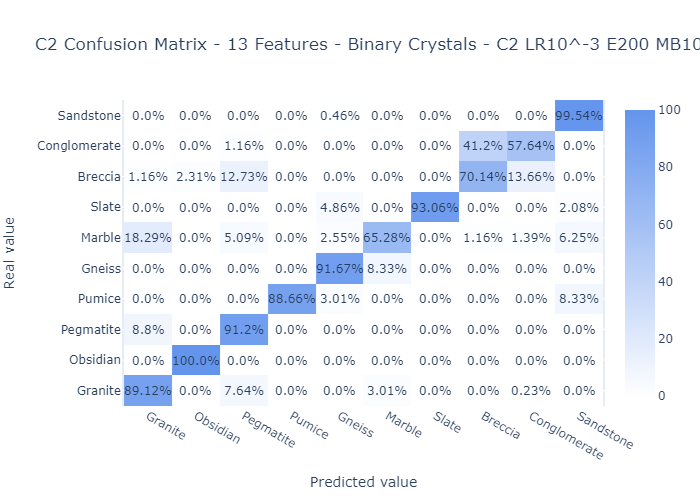
\includegraphics[width=0.9\textwidth, trim = 0cm 0cm 0.5cm 3.5cm, clip]{images/C2 Confusion Matrix - 13 Features - Binary Crystals.png}
    \caption{Sequential CBM Network Accuracy Confusion Matrix - 13 Features - Binary Crystal Ratings} \label{fig:Sequential CBM Network Accuracy Confusion Matrix - 13 Features - Binary Crystal Ratings}
\end{figure}

\begin{figure}[H]
  \centering
    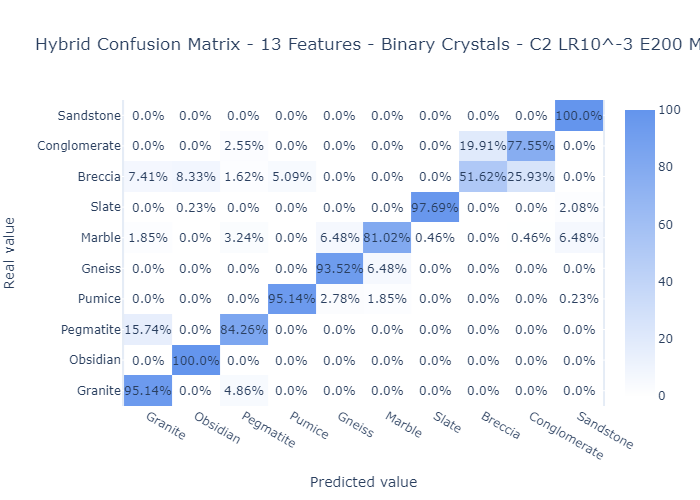
\includegraphics[width=0.9\textwidth, trim = 0cm 0cm 0.5cm 3.5cm, clip]{images/Hybrid Confusion Matrix- 13 Features - Binary Crystals.png}
    \caption{Hybrid Network Accuracy Confusion Matrix - 13 Features - Binary Crystal Ratings} \label{fig:Hybrid Network Accuracy -  13 Features - Binary Crystal Ratings - Confusion Matrix}
\end{figure}

\subsection{13 Features - Continuous Crystal Rating}

\begin{figure}[H]
  \centering
    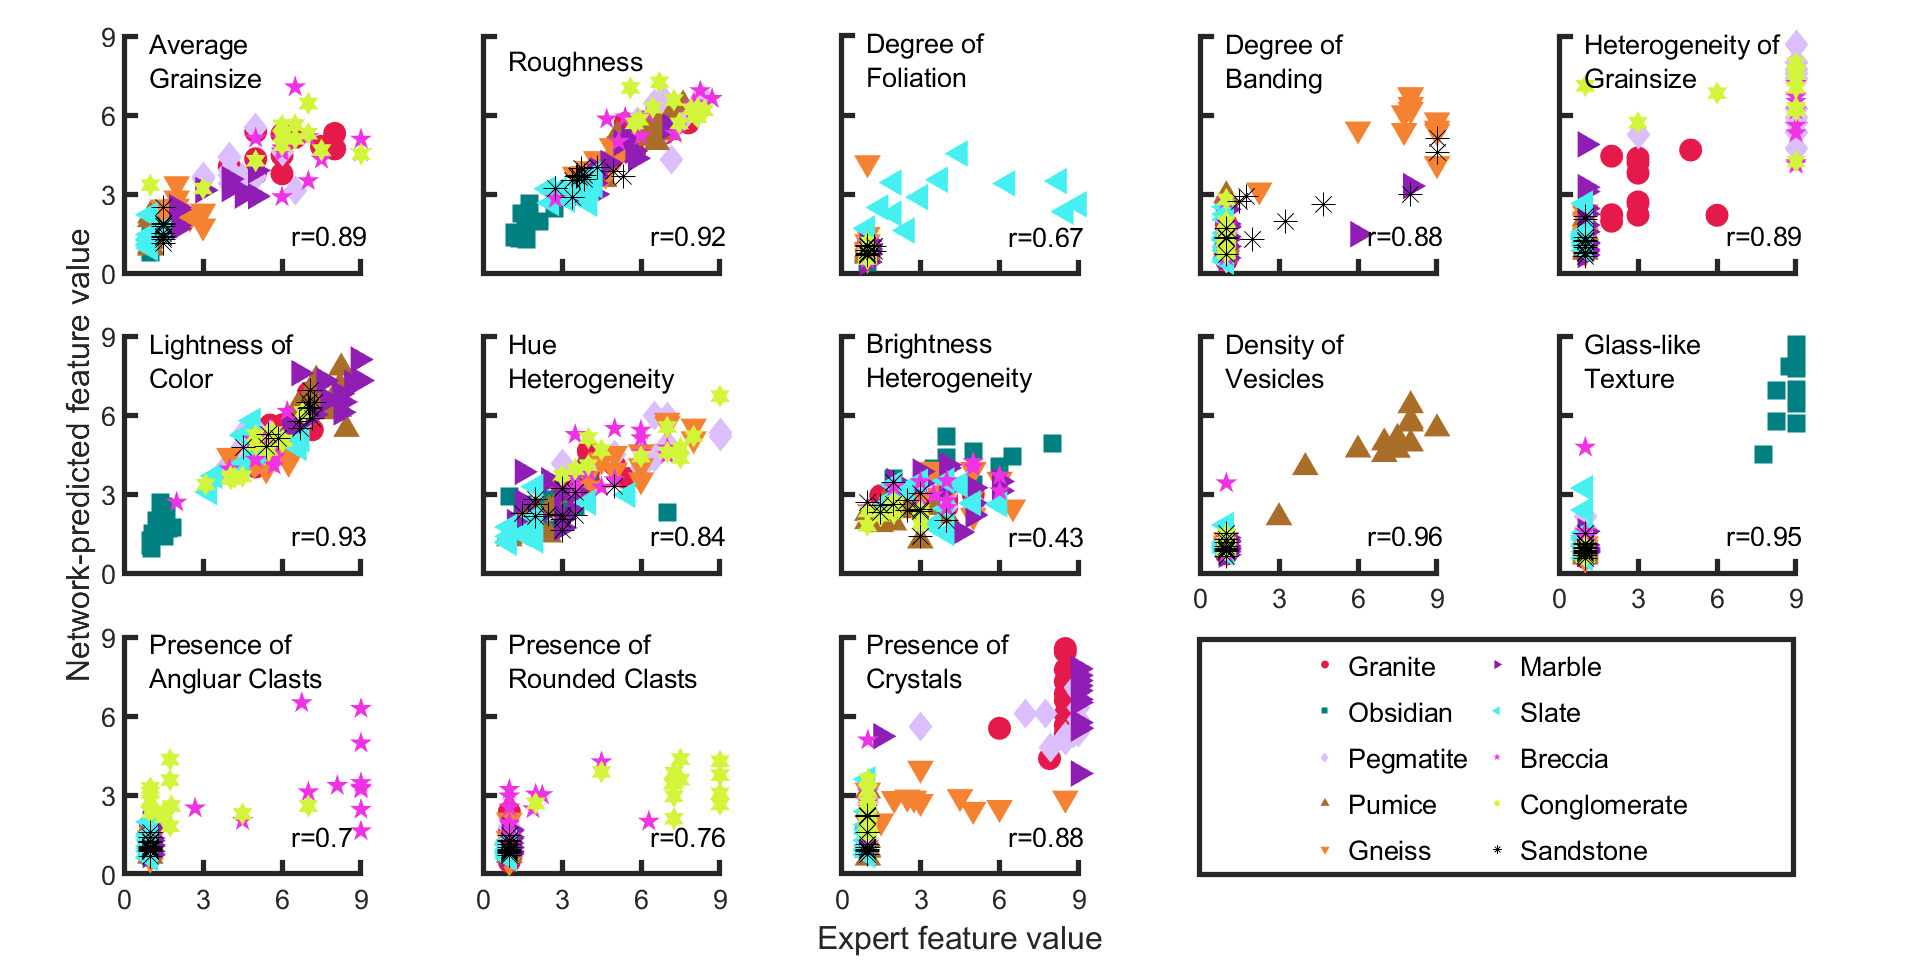
\includegraphics[width=\textwidth]{images/MATLAB Correlation - C2_Vs_Expert - 13 Feautres - Continuous.png}
    \caption{Feature Correlation - Sequential CBM Vs Expert Ratings - 13 Features - Continuous Crystal Rating} \label{fig:Feature Correlation - Sequential CBM Vs Expert Ratings - 13 Features - Continuous Crystal Rating}
\end{figure}

\begin{figure}[H]
  \centering
    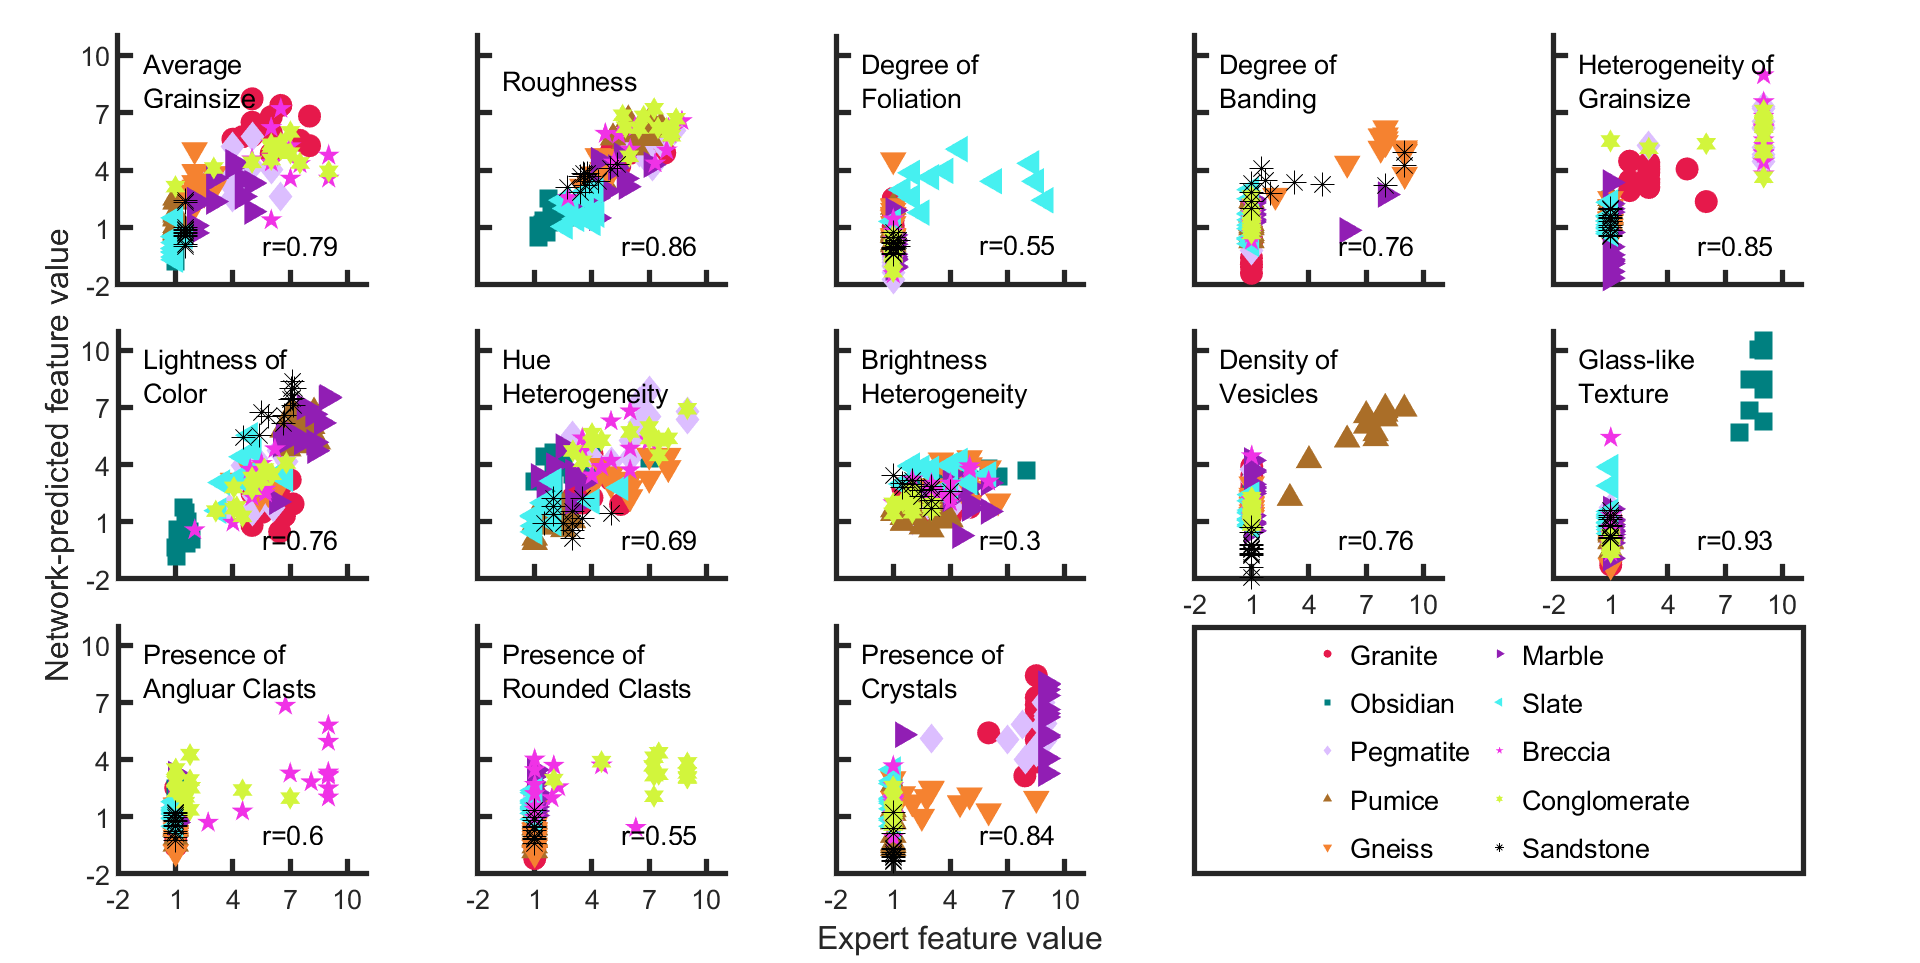
\includegraphics[width=\textwidth]{images/MATLAB Correlation - Hybrid_Vs_Expert - 13 Feautres - Continuous.png}
    \caption{Feature Correlation - Hybrid Sequential CBM Vs Expert Ratings - 13 Features - Continuous Crystal Rating} \label{fig:Feature Correlation - Hybrid Sequential CBM Vs Expert Ratings - 13 Features - Continuous Crystal Rating}
\end{figure}

\begin{figure}[H]
  \centering
    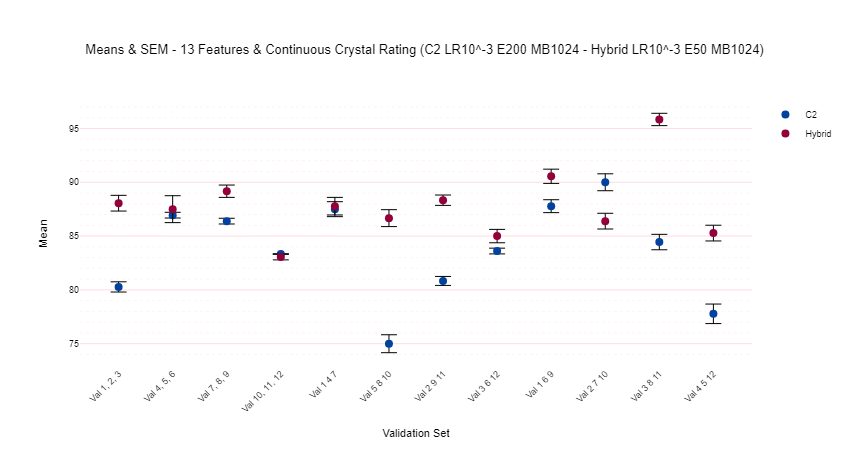
\includegraphics[width=\textwidth]{images/Means & SEM - 13 Features & Continuous Crystal Rating (C2 LR10^-3 E200 MB1024 - Hybrid LR10^-3 E50 MB1024).png}
    \caption{Means \& SEM - Validation Sets - 13 Features - Continuous Crystal Rating} \label{fig:Means & SEM - Validation Sets - 13 Features - Continuous Crystal Rating}
\end{figure}


\begin{figure}[H]
  \centering
    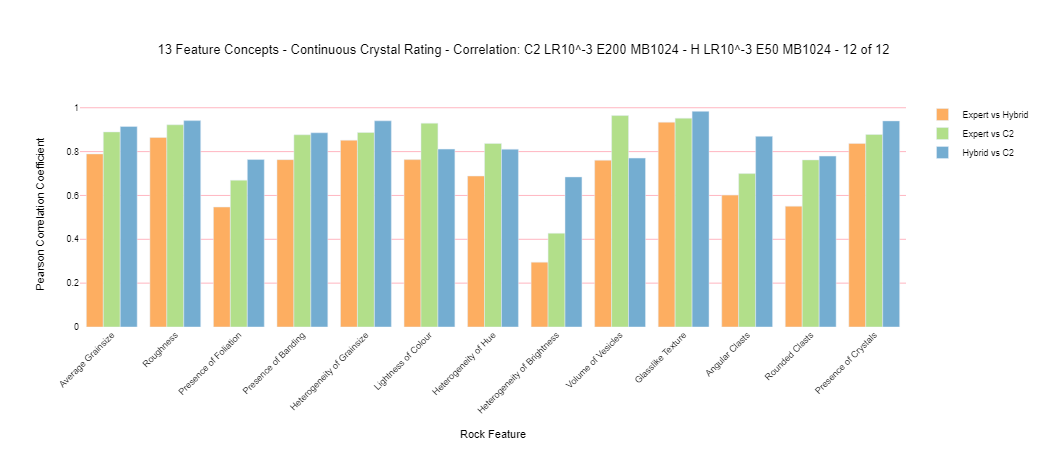
\includegraphics[width=\textwidth]{images/13 Feature Concepts - Continuous Crystal Rating - Correlation- C2 LR10^-3 E200 MB1024 - H LR10^-3 E50 MB1024 - 12 of 12.png}
    \caption{13 Feature Concepts - Continuous Crystal Rating - Mean correlation of Feature Concepts} \label{fig:13 Feature Concepts - Continuous Crystal Rating - Mean correlation of Feature Concepts}
\end{figure}


\begin{figure}[H]
  \centering
    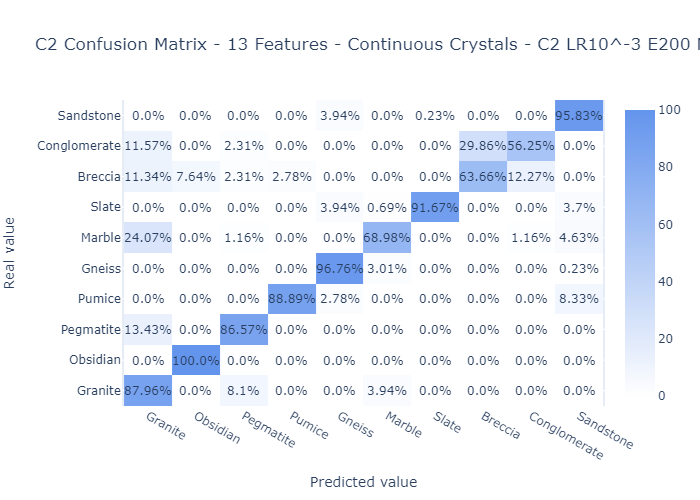
\includegraphics[width=0.9\textwidth, trim = 0cm 0cm 0.5cm 3.5cm, clip]{images/C2 Confusion Matrix - 13 Features - Continuous Crystals.png}
    \caption{Sequential CBM Network Accuracy Confusion Matrix - 13 Features - Continuous Crystal Ratings} \label{fig:Sequential CBM Network Accuracy Confusion Matrix - 13 Features - Continuous Crystal Ratings}
\end{figure}

\begin{figure}[H]
  \centering
    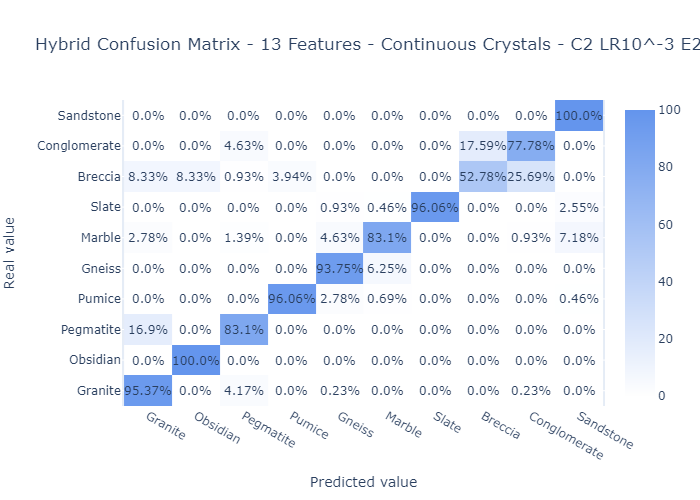
\includegraphics[width=0.9\textwidth, trim = 0cm 0cm 0.5cm 3.5cm, clip]{images/Hybrid Confusion Matrix - 13 Features - Continuous Crystals.png}
    \caption{Hybrid Network Accuracy Confusion Matrix- 13 Features - Continuous Crystal Ratings} \label{fig:Hybrid Network Accuracy Confusion Matrix- 13 Features - Continuous Crystal Ratings}
\end{figure}

\subsection{12 Features ("Heterogeneity of Brightness" Feature Removed) - Binary Crystal Rating}

\begin{figure}[H]
  \centering
    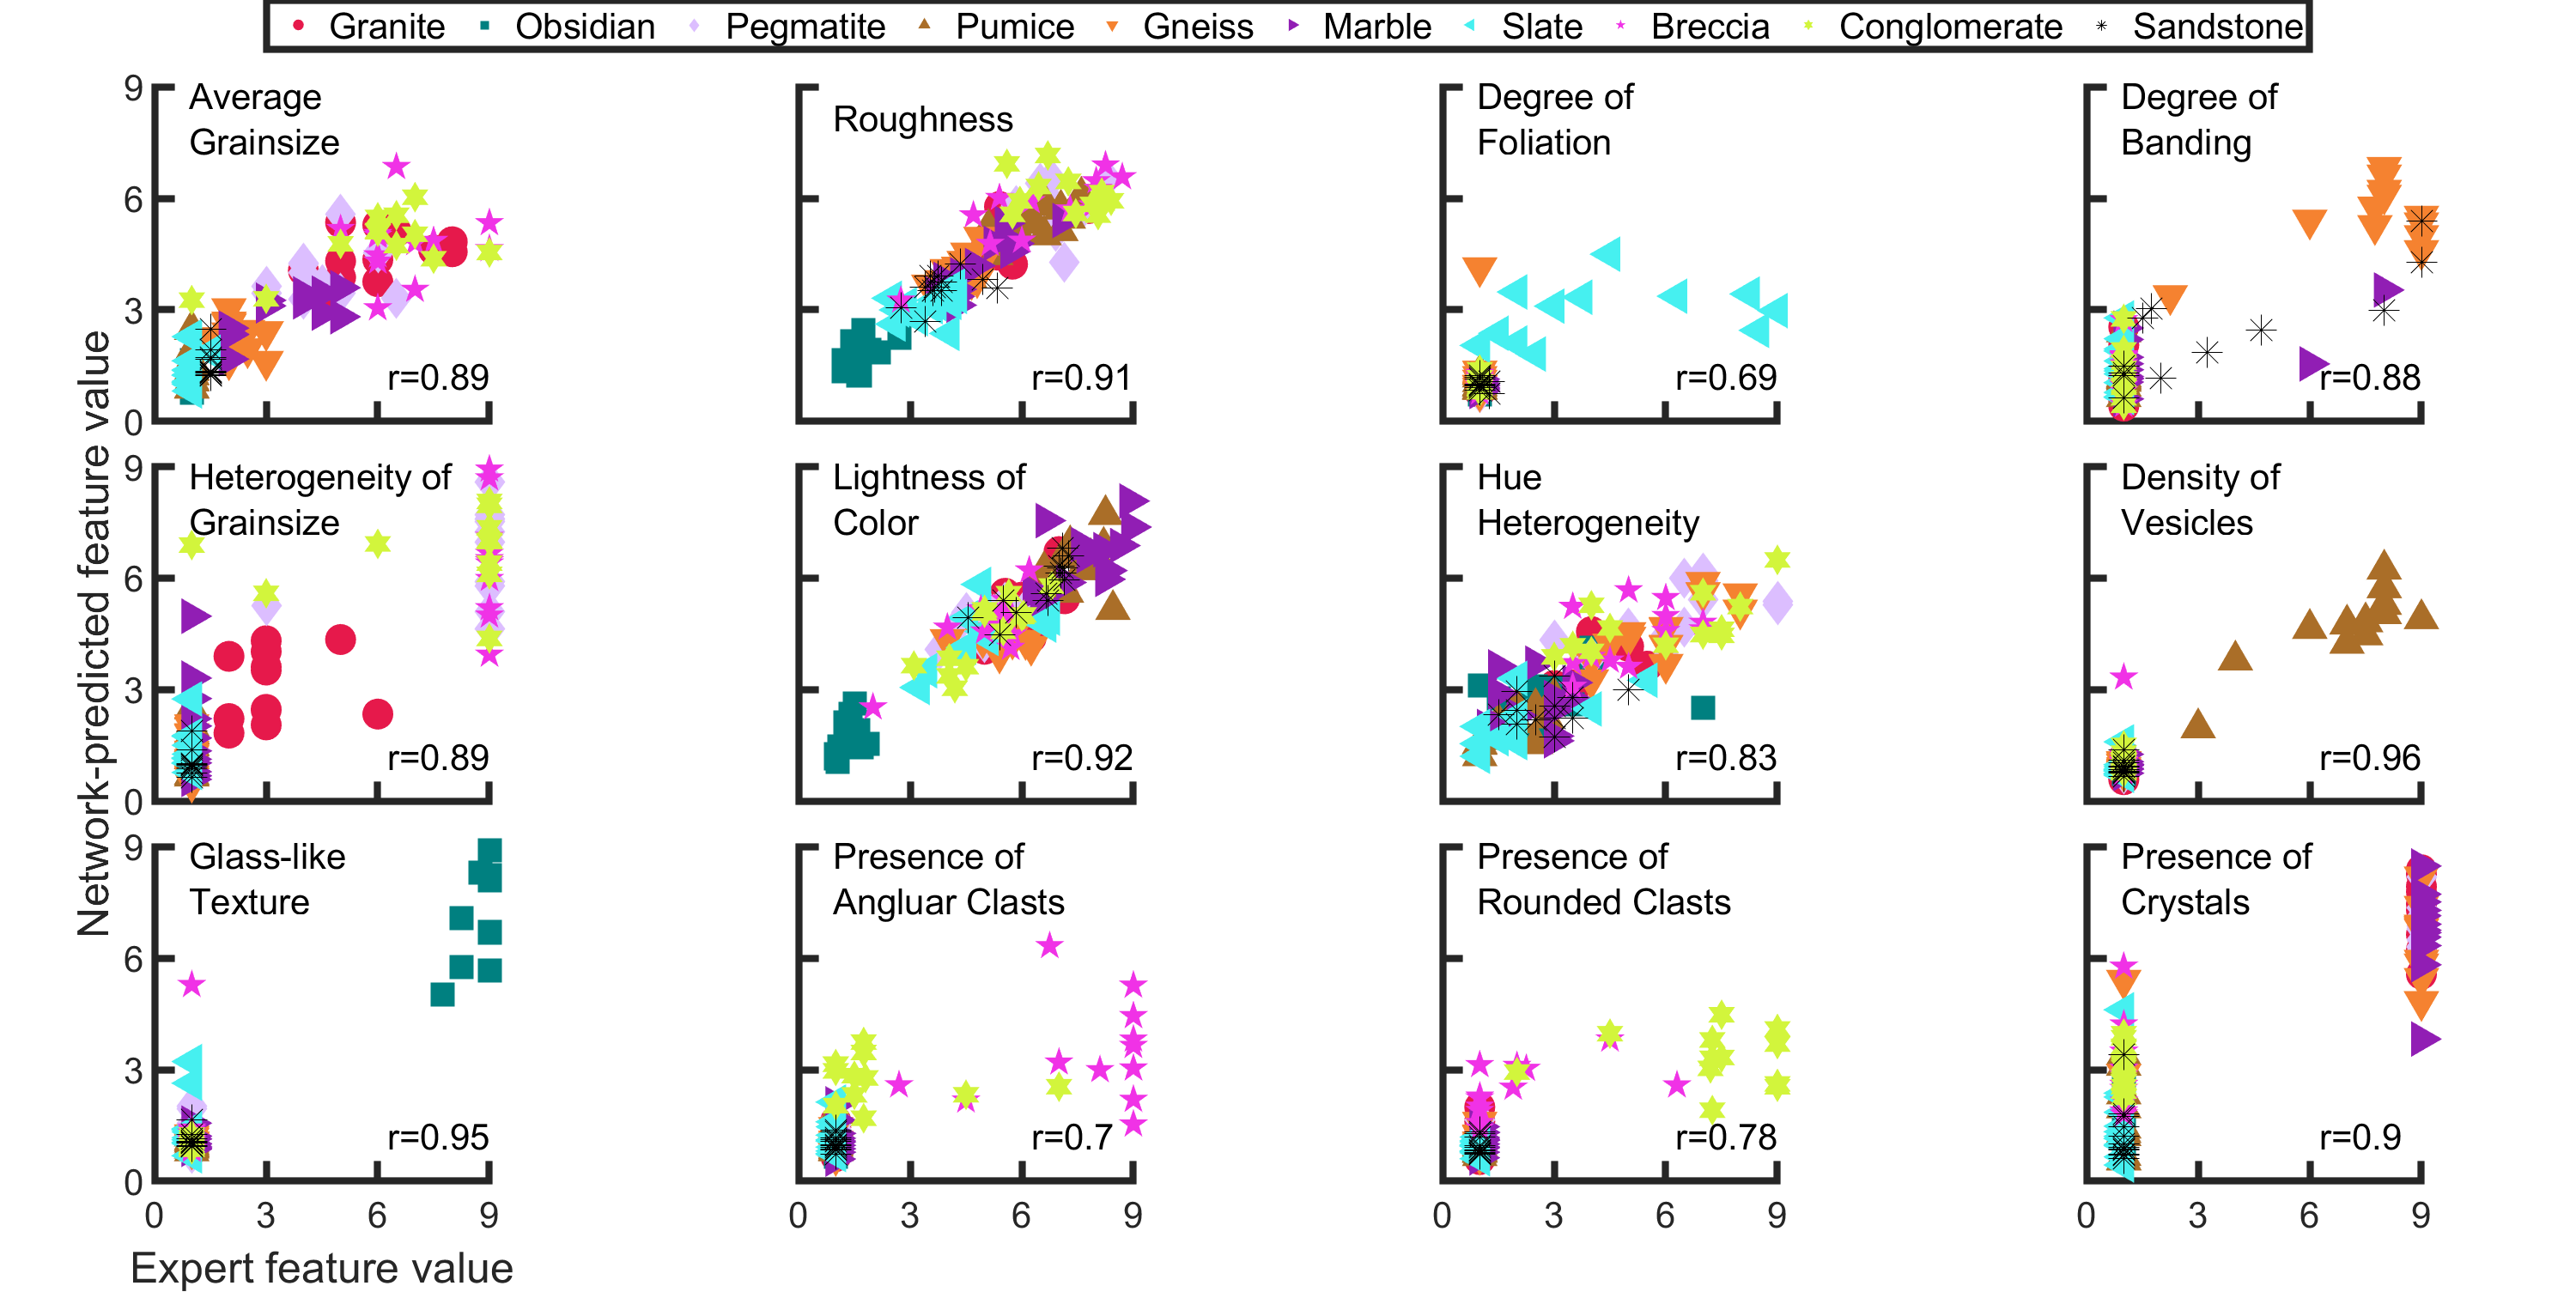
\includegraphics[width=\textwidth]{images/MATLAB Correlation - C2_Vs_Expert - 12 Feautres - Binary.png}
    \caption{Feature Correlation - Sequential CBM Vs Expert Ratings - 12 Features - Binary Crystal Rating} \label{fig:Feature Correlation - Sequential CBM Vs Expert Ratings - 12 Features - Binary Crystal Rating}
\end{figure}

\begin{figure}[H]
  \centering
    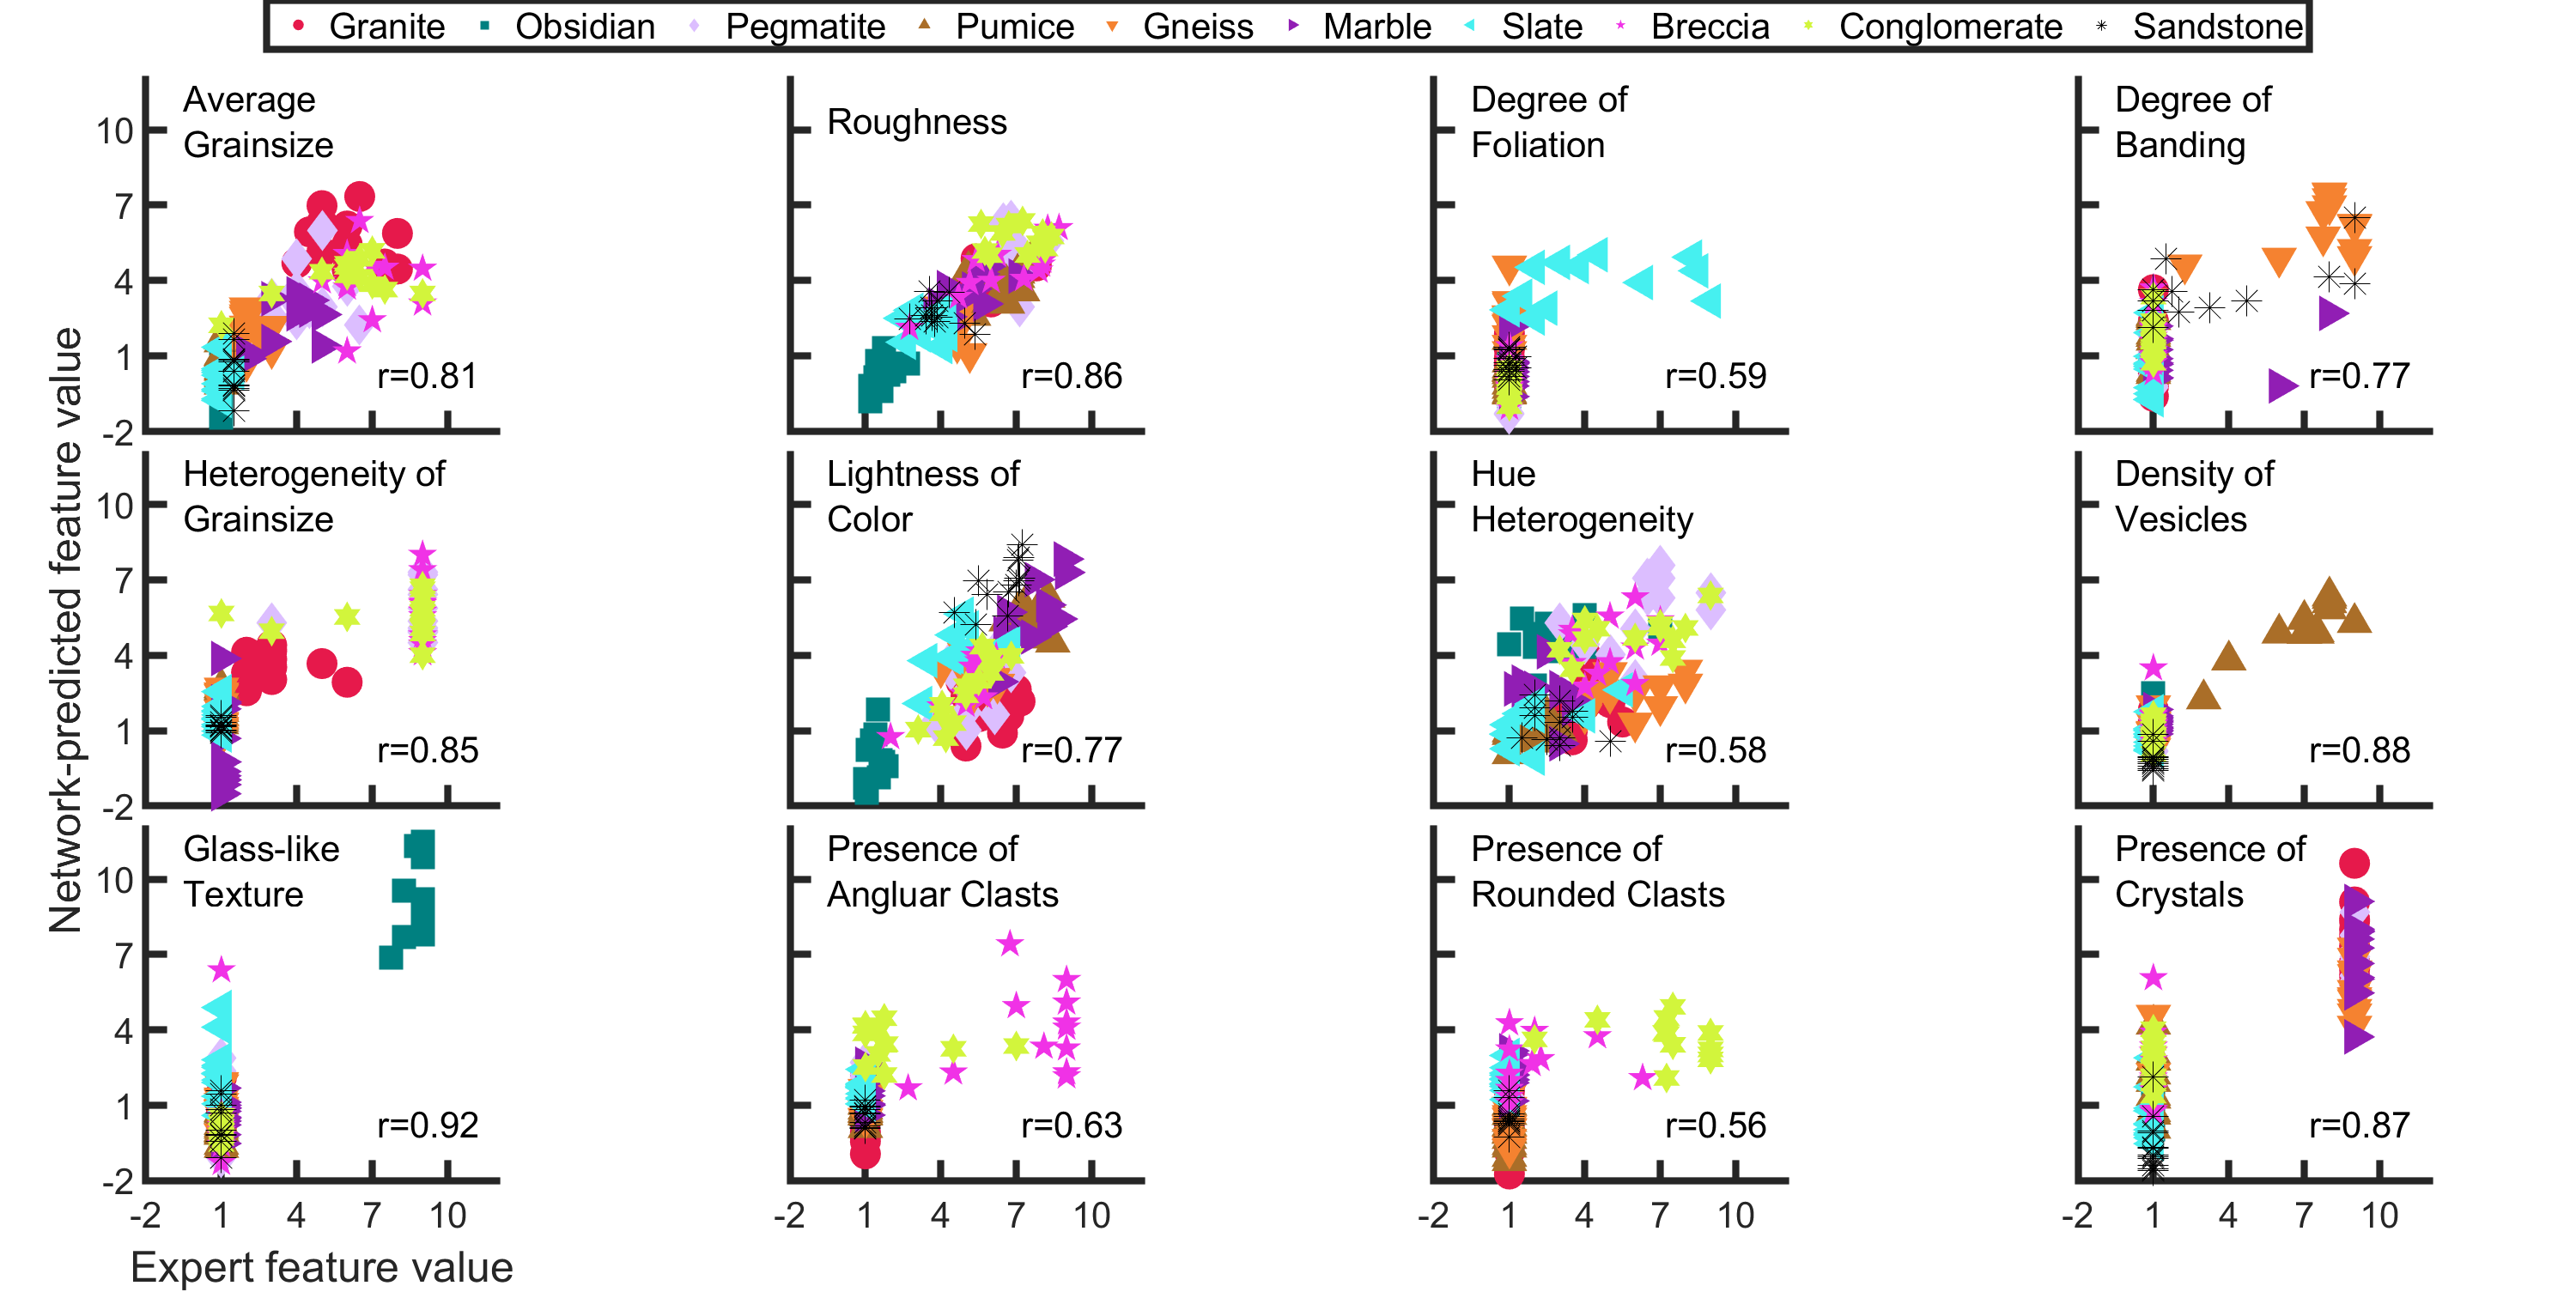
\includegraphics[width=\textwidth]{images/MATLAB Correlation - Hybrid_Vs_Expert - 12 Feautres - Binary.png}
    \caption{Feature Correlation - Hybrid Sequential CBM Vs Expert Ratings - 12 Features - Binary Crystal Rating} \label{fig:Feature Correlation - Hybrid Sequential CBM Vs Expert Ratings - 12 Features - Binary Crystal Rating}
\end{figure}

\begin{figure}[H]
  \centering
    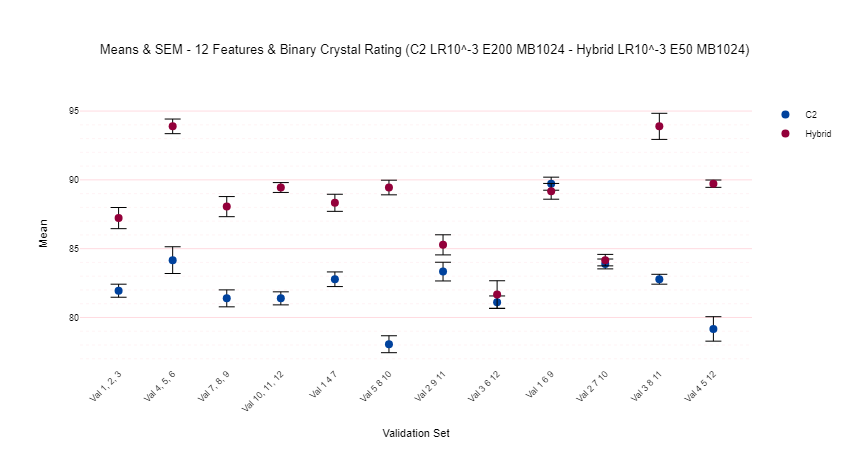
\includegraphics[width=\textwidth]{images/Means & SEM - 12 Features & Binary Crystal Rating (C2 LR10^-3 E200 MB1024 - Hybrid LR10^-3 E50 MB1024).png}
    \caption{Means \& SEM - Validation Sets - 12 Features - Binary Crystal Rating} \label{fig:Means & SEM - Validation Sets - 12 Features - Binary Crystal Rating}
\end{figure}


\begin{figure}[H]
  \centering
    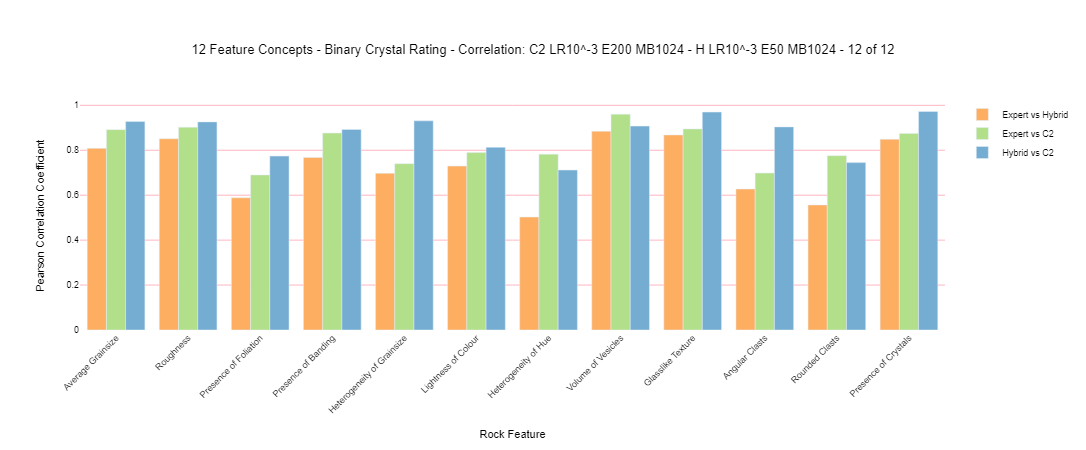
\includegraphics[width=\textwidth]{images/12 Feature Concepts - Binary Crystal Rating - Correlation- C2 LR10^-3 E200 MB1024 - H LR10^-3 E50 MB1024 - 12 of 12.png}
    \caption{12 Feature Concepts - Binary Crystal Rating - Mean correlation of Feature Concepts} \label{fig:12 Feature Concepts - Binary Crystal Rating - Mean correlation of Feature Concepts}
\end{figure}

\begin{figure}[H]
  \centering
    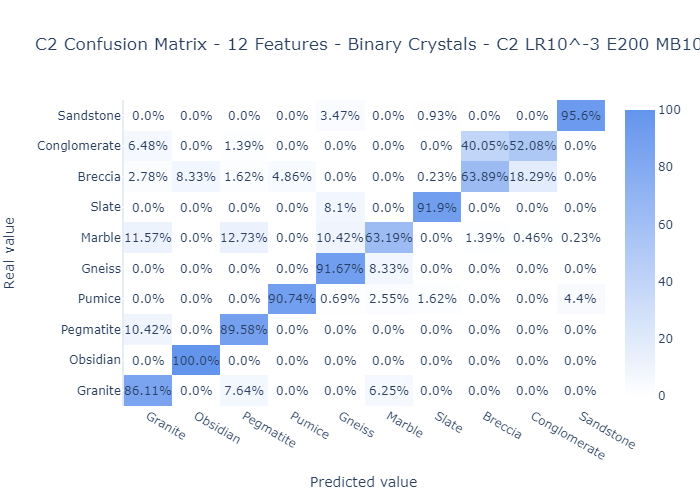
\includegraphics[width=0.9\textwidth, trim = 0cm 0cm 0.5cm 3.5cm, clip]{images/C2 Confusion Matrix - 12 Features - Binary Crystals.png}
    \caption{Sequential CBM Network Accuracy Confusion Matrix - 12 Features - Binary Crystal Ratings} \label{fig:Sequential CBM Network Accuracy Confusion Matrix - 12 Features - Binary Crystal Ratings}
\end{figure}

\begin{figure}[H]
  \centering
    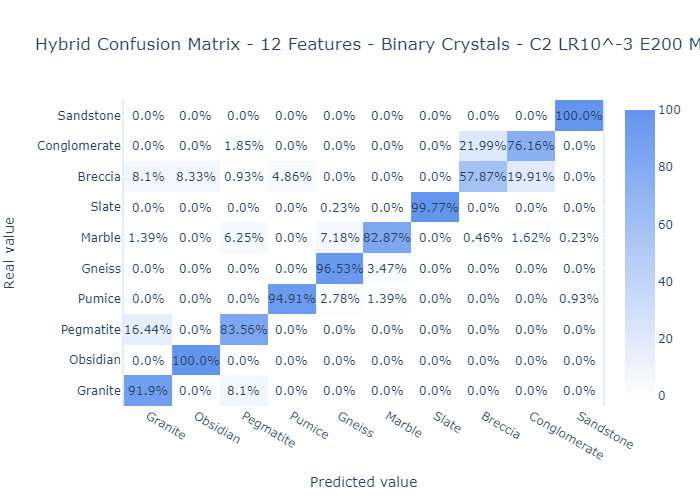
\includegraphics[width=0.9\textwidth, trim = 0cm 0cm 0.5cm 3.5cm, clip]{images/Hybrid Confusion Matrix - 12 Features - Binary Crystals.png }
    \caption{Hybrid Network Accuracy Confusion Matrix - 12 Features - Binary Crystal Ratings} \label{fig:Hybrid Network Accuracy Confusion Matrix- 12 Features - Binary Crystal Ratings}
\end{figure}

\subsection{12 Features ("Heterogeneity of Brightness" Feature Removed) - Continuous Crystal Rating}

\begin{figure}[H]
  \centering
    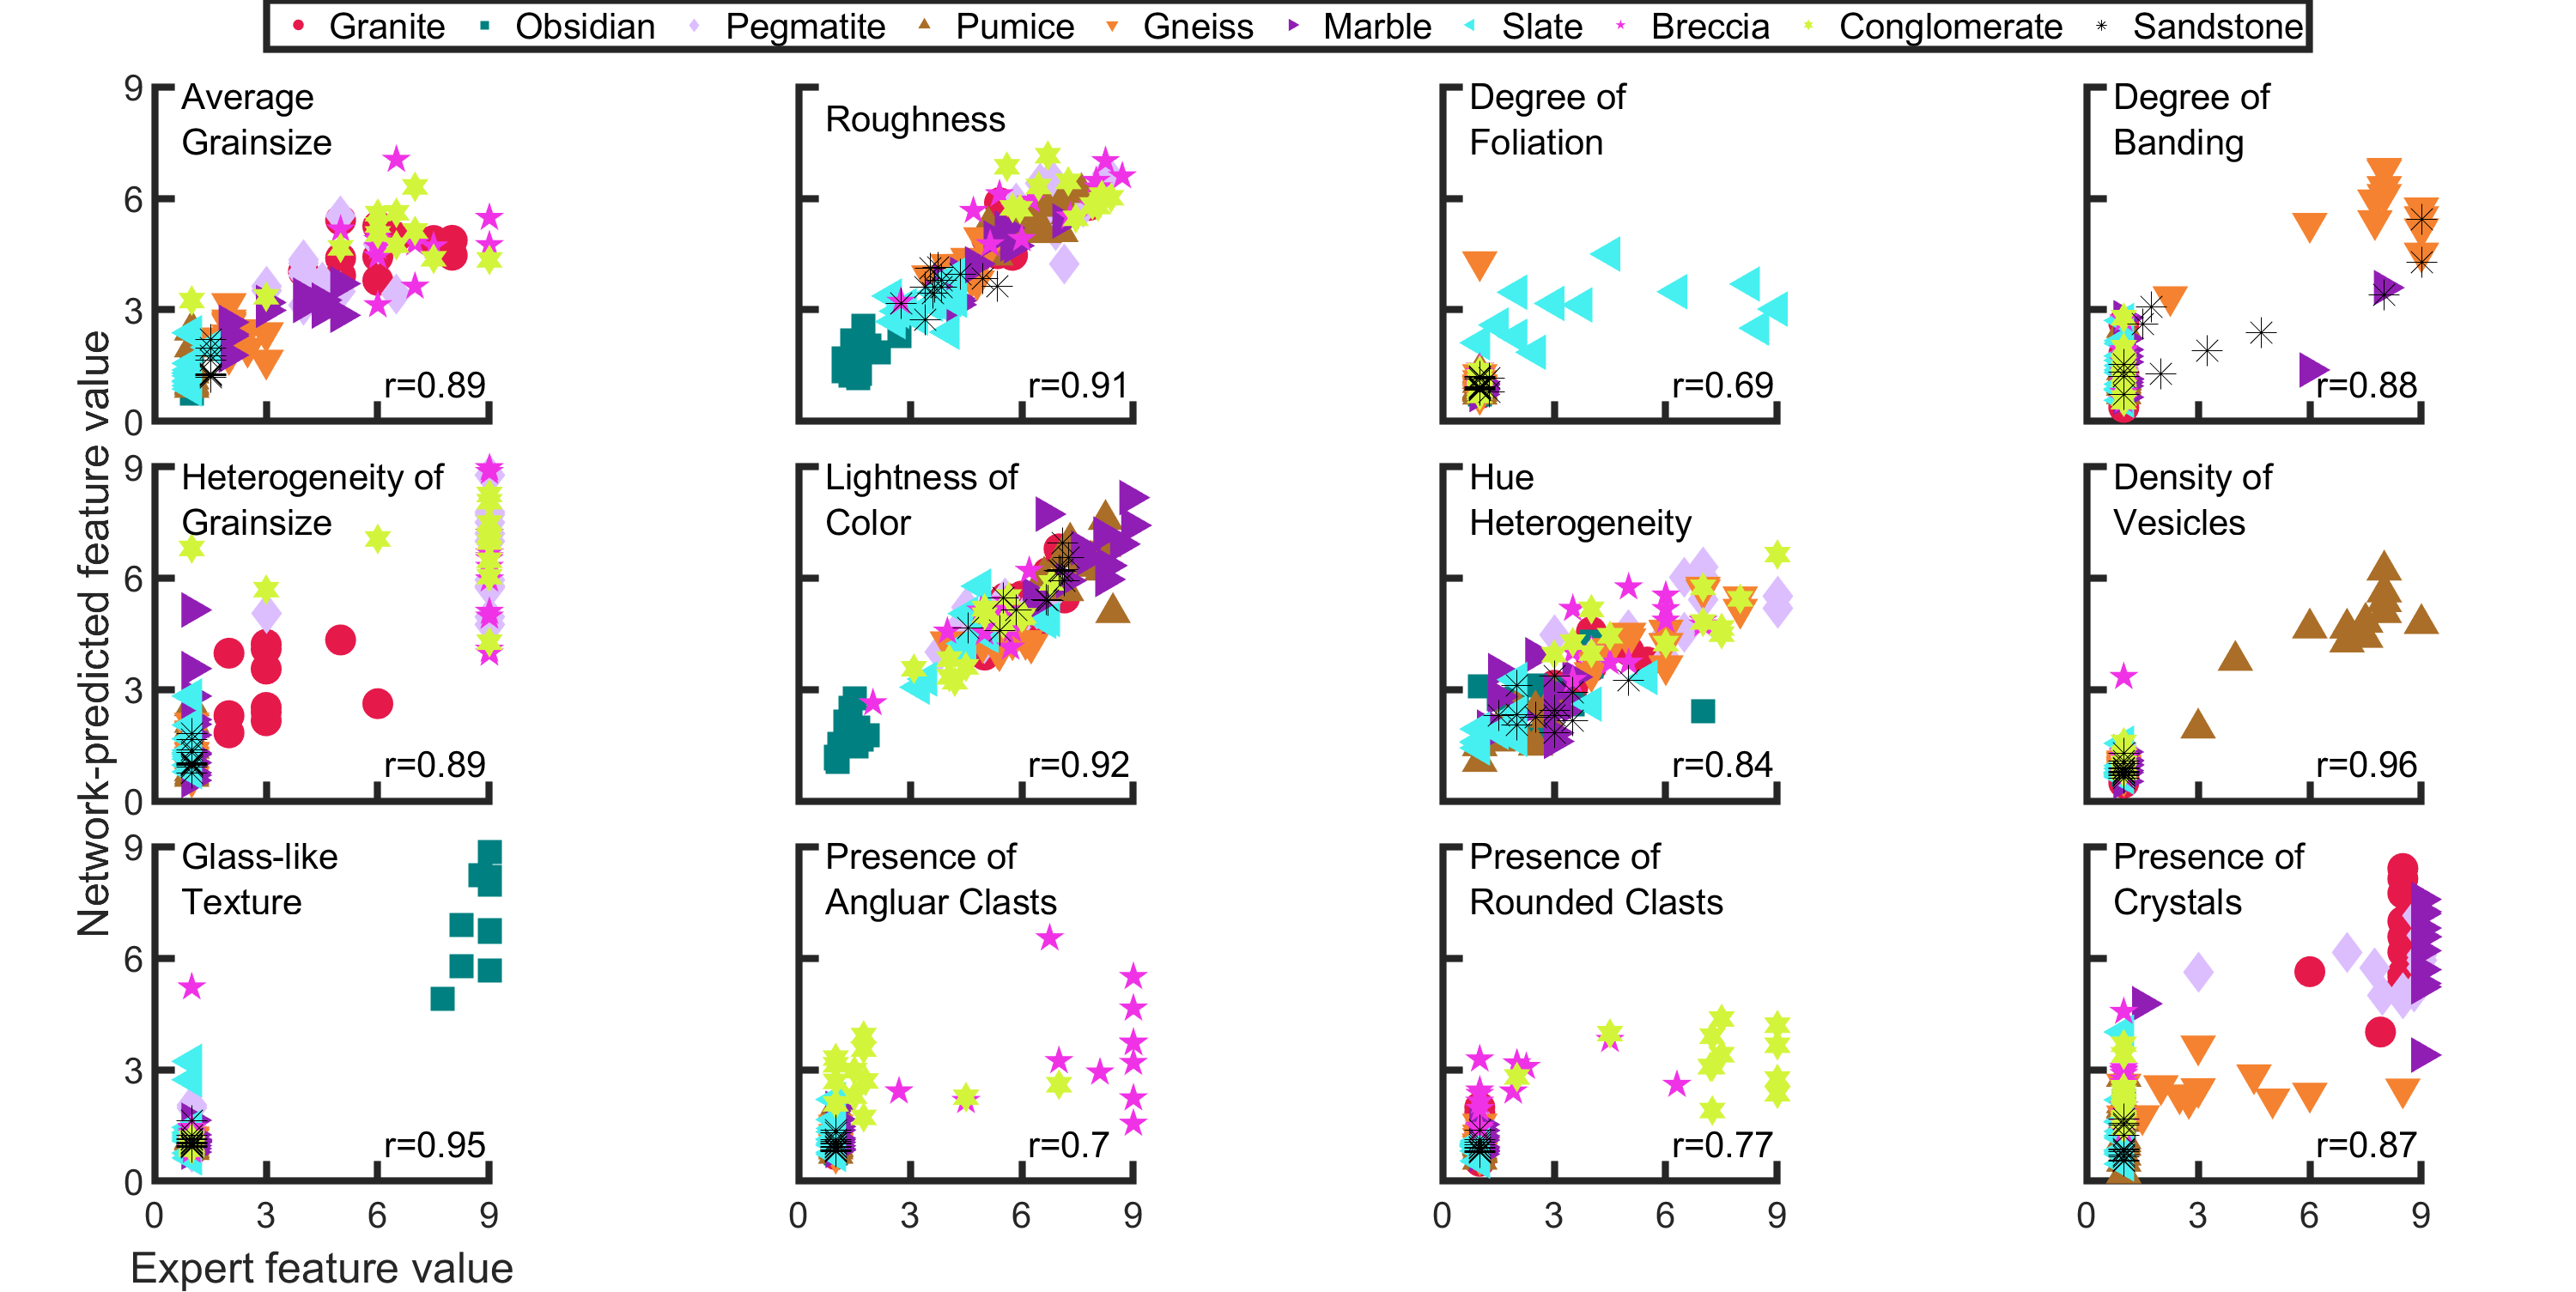
\includegraphics[width=\textwidth]{images/MATLAB Correlation - C2_Vs_Expert - 12 Feautres - Continuous.png}
    \caption{Feature Correlation - Sequential CBM Vs Expert Ratings - 12 Features - Continuous Crystal Rating} \label{fig:Feature Correlation - Sequential CBM Vs Expert Ratings - 12 Features - Continuous Crystal Rating}
\end{figure}

\begin{figure}[H]
  \centering
    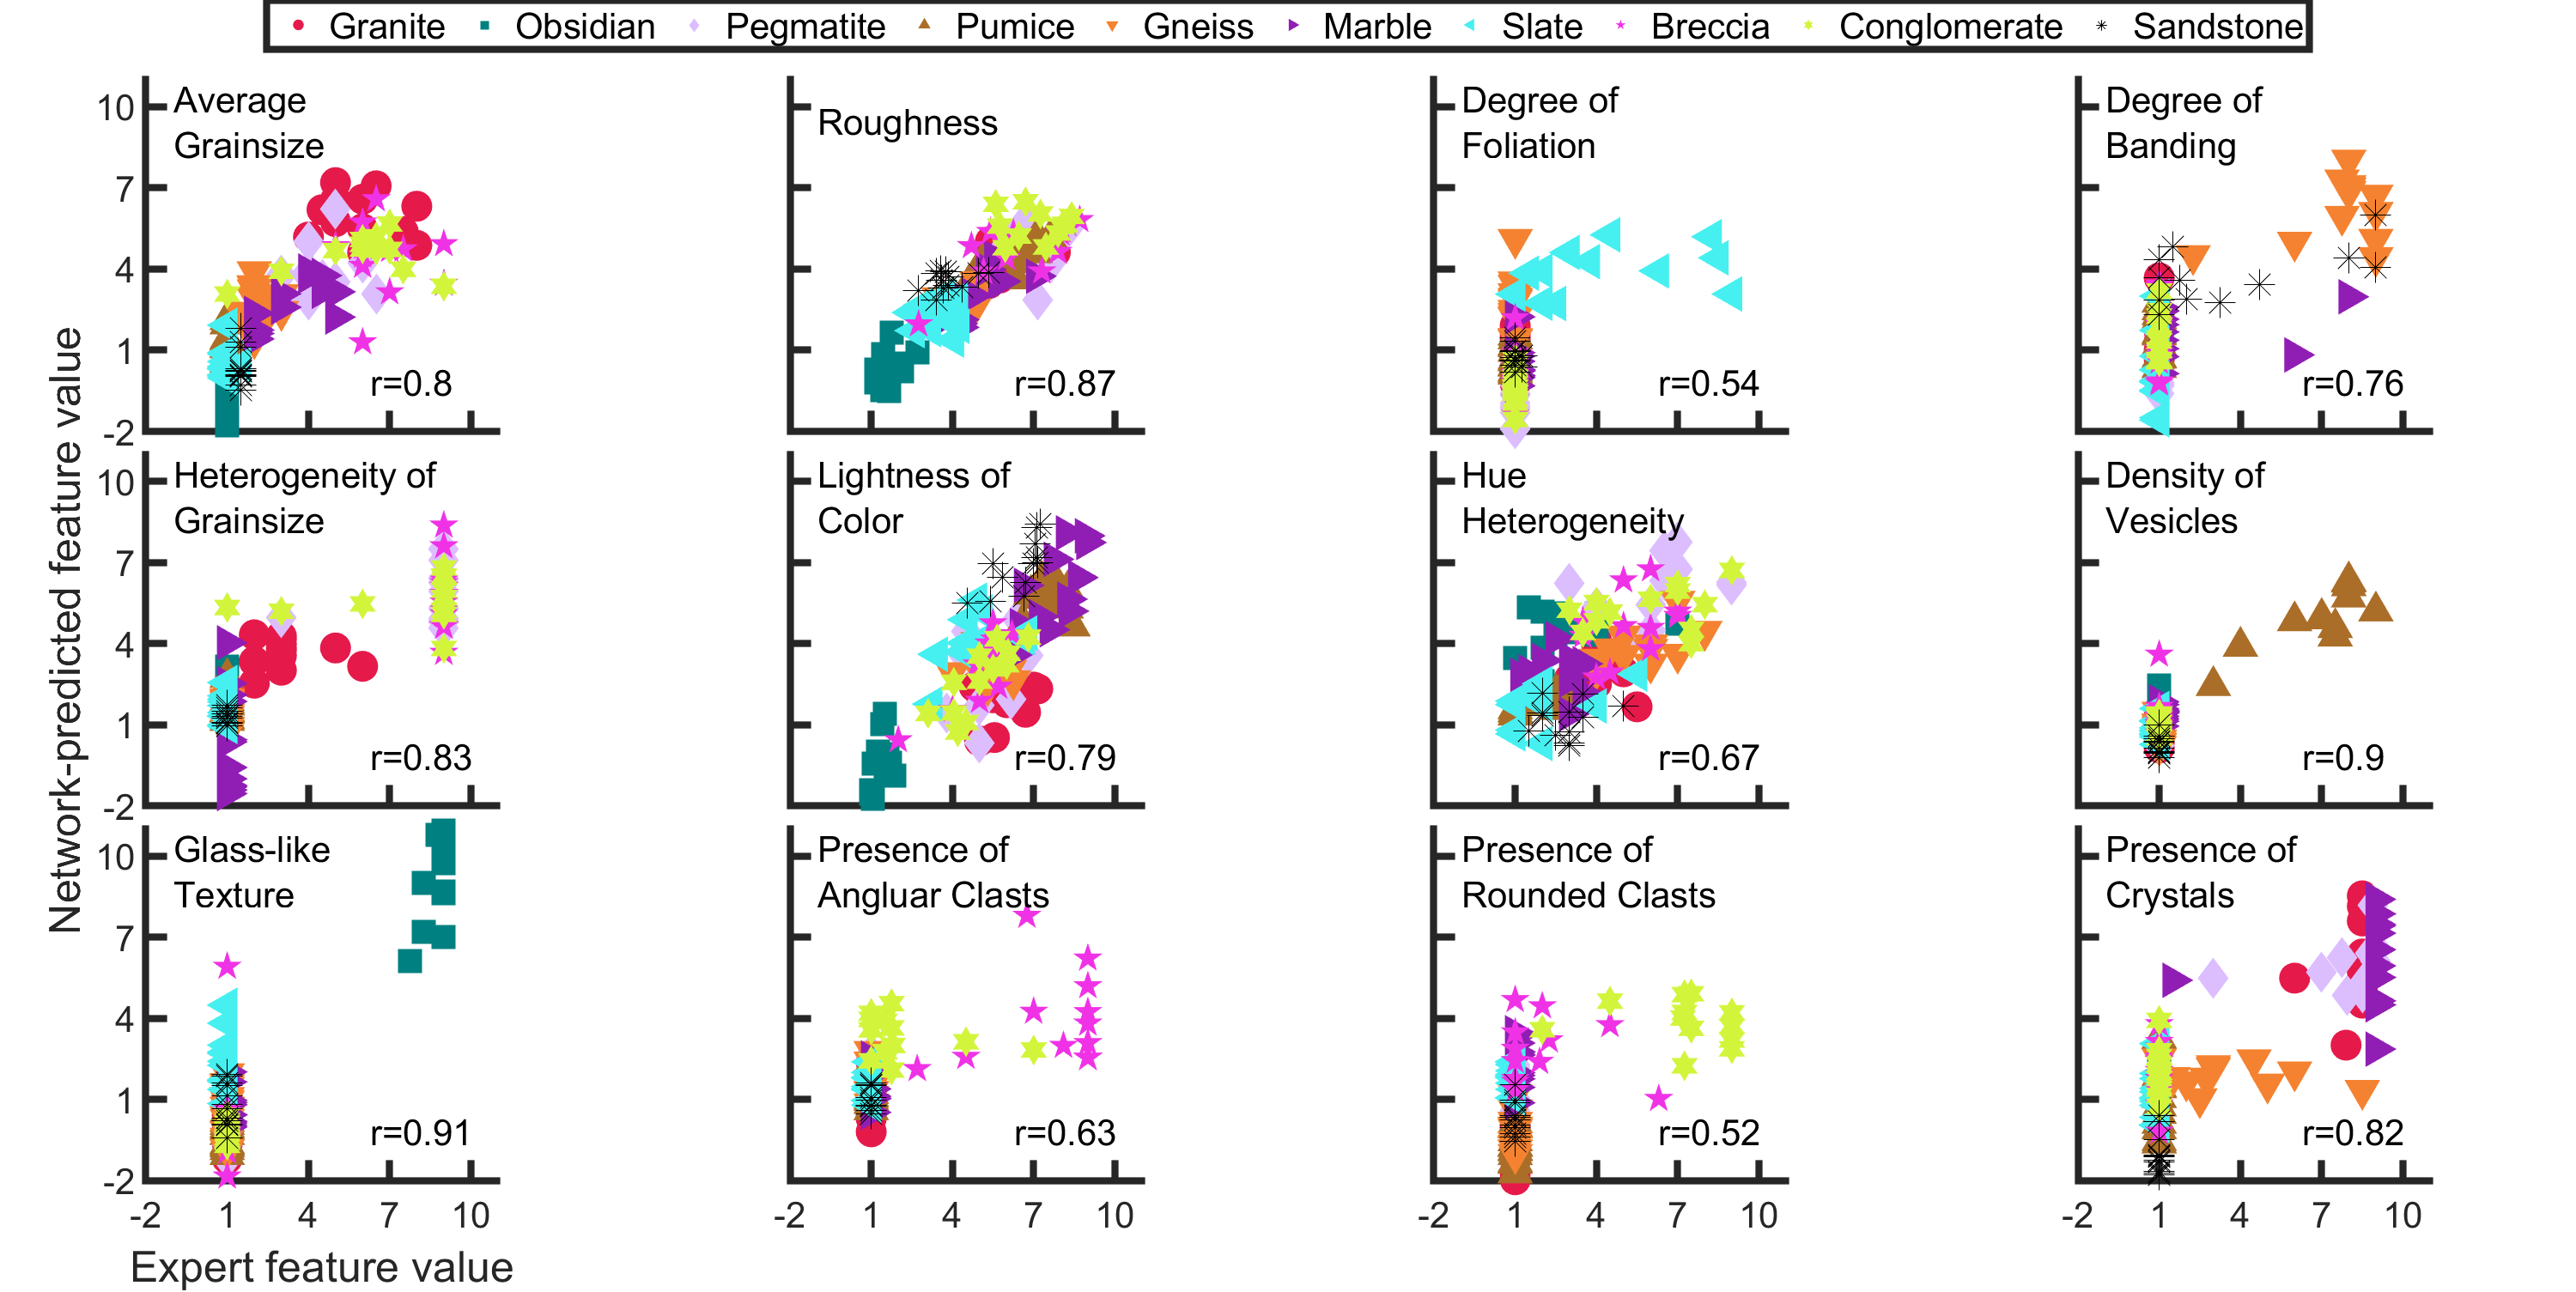
\includegraphics[width=\textwidth]{images/MATLAB Correlation - Hybrid_Vs_Expert - 12 Feautres - Continuous.png}
    \caption{Feature Correlation - Hybrid Sequential CBM Vs Expert Ratings - 12 Features - Continuous Crystal Rating} \label{fig:Feature Correlation - Hybrid Sequential CBM Vs Expert Ratings - 12 Features - Continuous Crystal Rating}
\end{figure}

\begin{figure}[H]
  \centering
    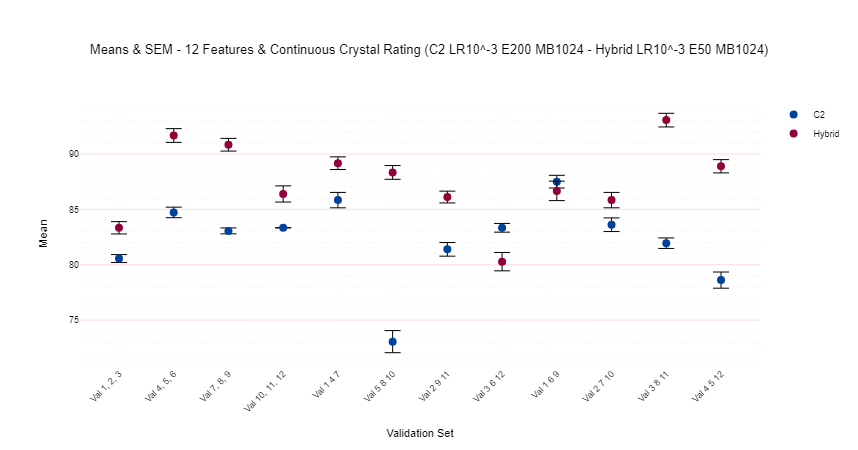
\includegraphics[width=\textwidth]{images/Means & SEM - 12 Features & Continuous Crystal Rating (C2 LR10^-3 E200 MB1024 - Hybrid LR10^-3 E50 MB1024).png}
    \caption{Means \& SEM - Validation Sets - 12 Features - Continuous Crystal Rating} \label{fig:Means & SEM - Validation Sets - 12 Features - Continuous Crystal Rating}
\end{figure}

\begin{figure}[H]
  \centering
    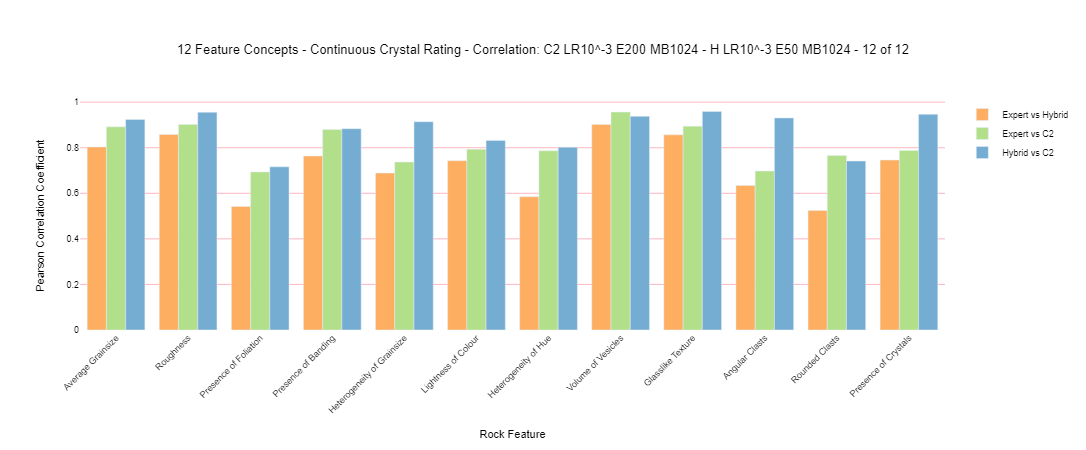
\includegraphics[width=\textwidth]{images/12 Feature Concepts - Continuous Crystal Rating - Correlation- C2 LR10^-3 E200 MB1024 - H LR10^-3 E50 MB1024 - 12 of 12.png}
    \caption{12 Feature Concepts - Continuous Crystal Rating - Mean correlation of Feature Concepts} \label{fig:12 Feature Concepts - Continuous Crystal Rating - Mean correlation of Feature Concepts}
\end{figure}


\begin{figure}[H]
  \centering
    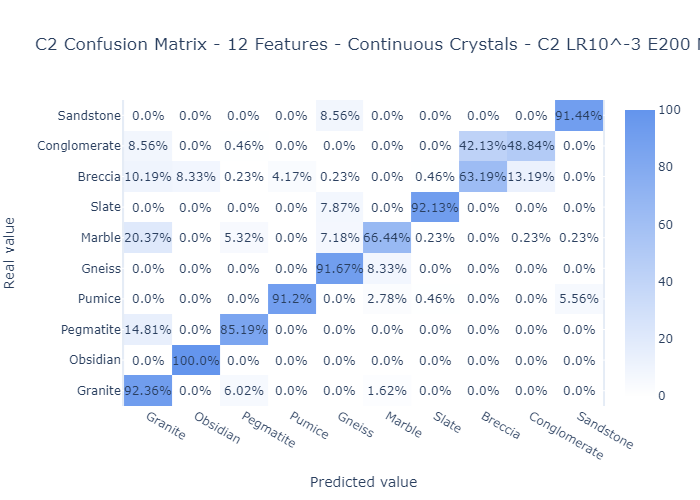
\includegraphics[width=\textwidth, trim = 0cm 0cm 0.5cm 3.5cm, clip]{images/C2 Confusion Matrix - 12 Features - Continuous Crystals.png}
    \caption{Sequential CBM Network Accuracy Confusion Matrix - 12 Features - Continuous Crystal Ratings} \label{fig:Sequential CBM Network Accuracy Confusion Matrix - 12 Features - Continuous Crystal Ratings}
\end{figure}

\begin{figure}[H]
  \centering
    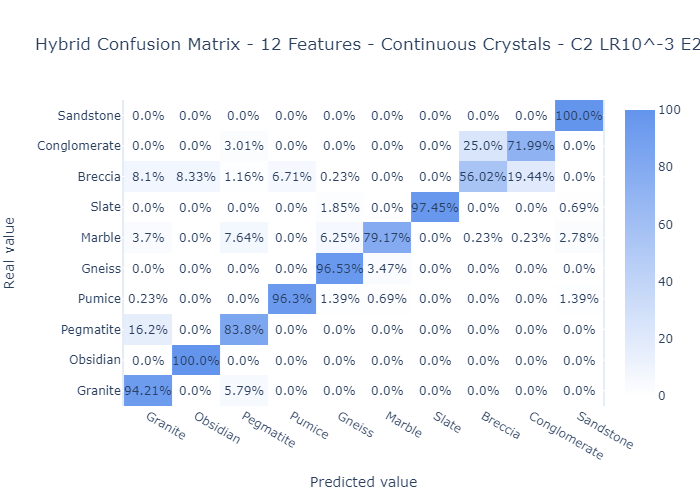
\includegraphics[width=0.9\textwidth, trim = 0cm 0cm 0.5cm 3.5cm, clip]{images/Hybrid Confusion Matrix - 12 Features - Continuous Crystals.png}
    \caption{Hybrid Network Accuracy Confusion Matrix - 12 Features - Continuous Crystal Ratings} \label{fig:Hybrid Network Accuracy Confusion Matrix- 12 Features - Continuous Crystal Ratings}
\end{figure}


\section{Tables}

\subsection{An Example of 13 Expert Feature Ratings for Granite Used for Training}
\scriptsize
\begin{longtable}[c]{@{}lllllllllllll@{}}
\toprule
%\addtolength{\tabcolsep}{-1pt}
\textbf{Rock   Type: Granite} &
   &
  \textbf{} &
  \textbf{} &
  \textbf{} &
  \textbf{} &
  \textbf{} &
  \textbf{} &
  \textbf{} &
  \textbf{} &
  \textbf{} &
  \textbf{} &
  \textbf{} \\
\endfirsthead
%
\multicolumn{13}{c}%
{{\bfseries Table \thetable\ continued from previous page}} \\
\endhead
%
 &
  \multicolumn{12}{c}{\textbf{Rock Image Instance}} \\
\multicolumn{1}{c}{\textbf{Feature}} &
  \cellcolor[HTML]{FFD966}\textbf{1} &
  \cellcolor[HTML]{FFD966}\textbf{2} &
  \cellcolor[HTML]{FFD966}\textbf{3} &
  \cellcolor[HTML]{FFD966}\textbf{4} &
  \cellcolor[HTML]{FFD966}\textbf{5} &
  \cellcolor[HTML]{FFD966}\textbf{6} &
  \cellcolor[HTML]{FFD966}\textbf{7} &
  \cellcolor[HTML]{FFD966}\textbf{8} &
  \cellcolor[HTML]{FFD966}\textbf{9} &
  \cellcolor[HTML]{FFD966}\textbf{10} &
  \cellcolor[HTML]{FFD966}\textbf{11} &
  \cellcolor[HTML]{FFD966}\textbf{12} \\
\cellcolor[HTML]{E2EFDA}\textbf{Average   Grainsize} &
  6.5 &
  4 &
  6 &
  4.5 &
  6 &
  5 &
  5 &
  5 &
  7.5 &
  6 &
  8 &
  8 \\
\cellcolor[HTML]{E2EFDA}\textbf{Roughness} &
  6.25 &
  5.3 &
  5.45 &
  5.35 &
  6.9 &
  5.15 &
  5.75 &
  5.05 &
  7.8 &
  6 &
  5.4 &
  5.65 \\
\cellcolor[HTML]{E2EFDA}\textbf{Presence of   Foliation} &
  1 &
  1 &
  1 &
  1 &
  1 &
  1 &
  1 &
  1 &
  1 &
  1 &
  1 &
  1 \\
\cellcolor[HTML]{E2EFDA}\textbf{Presence of   Banding} &
  1 &
  1 &
  1 &
  1 &
  1 &
  1 &
  1 &
  1 &
  1 &
  1 &
  1 &
  1 \\
\cellcolor[HTML]{E2EFDA}\textbf{Heterogeneity   of Grainsize} &
  3 &
  3 &
  6 &
  2 &
  3 &
  3 &
  2 &
  3 &
  5 &
  2 &
  3 &
  3 \\
\cellcolor[HTML]{E2EFDA}\textbf{Lightness of   Color} &
  5 &
  7.15 &
  6.25 &
  6 &
  5 &
  5.55 &
  6.45 &
  6.7 &
  4.8 &
  5.5 &
  7 &
  6.5 \\
\cellcolor[HTML]{E2EFDA}\textbf{Heterogeneity   of Hue} &
  5 &
  3 &
  4 &
  3.5 &
  4 &
  3.5 &
  3 &
  3 &
  4 &
  5.5 &
  4 &
  4 \\
\cellcolor[HTML]{E2EFDA}\textbf{Heterogeneity   of Brightness} &
  4 &
  5 &
  3 &
  5 &
  1.5 &
  2 &
  4 &
  3 &
  3 &
  2 &
  4 &
  2.5 \\
\cellcolor[HTML]{E2EFDA}\textbf{Volume of   Vesicles} &
  1 &
  1 &
  1 &
  1 &
  1 &
  1 &
  1 &
  1 &
  1 &
  1 &
  1 &
  1 \\
\cellcolor[HTML]{E2EFDA}\textbf{Glasslike   texture} &
  1 &
  1 &
  1 &
  1 &
  1 &
  1 &
  1 &
  1 &
  1 &
  1 &
  1 &
  1 \\
\cellcolor[HTML]{E2EFDA}\textbf{Angular Clasts} &
  1 &
  1 &
  1 &
  1 &
  1 &
  1 &
  1 &
  1 &
  1 &
  1 &
  1 &
  1 \\
\cellcolor[HTML]{E2EFDA}\textbf{Rounded Clasts} &
  1 &
  1 &
  1 &
  1 &
  1 &
  1 &
  1 &
  1 &
  1 &
  1 &
  1 &
  1 \\
\cellcolor[HTML]{E2EFDA}\textbf{Presence of   Crystals} &
  8.5 &
  8.5 &
  6 &
  8.5 &
  7.9 &
  8.5 &
  8.5 &
  8.5 &
  8.5 &
  8.5 &
  8.5 &
  8.5
\\
\caption{An Example of 13 Expert Feature Ratings for Granite - As Used for Training}
\label{An Example of 13 Expert Feature Ratings for Granite - As Used for Training}\\
\end{longtable}


\subsection{Feature Correlations - 13 Features - Continuous (Scalar) Crystal Rating 12 Runs of 12 Alternating Validation Sets}
\scriptsize
\begin{longtable}[c]{@{}llllllllll@{}}
\toprule
\addtolength{\tabcolsep}{-1pt}
\textbf{Set/Runs} &
  \cellcolor[HTML]{FCE4D6}\textbf{12/12} &
  \cellcolor[HTML]{FCE4D6}\textbf{12/12} &
  \cellcolor[HTML]{FCE4D6}\textbf{12/12} &
  \cellcolor[HTML]{FCE4D6}\textbf{12/12} &
  \cellcolor[HTML]{FCE4D6}\textbf{12/12} &
  \cellcolor[HTML]{FCE4D6}\textbf{12/12} &
  \cellcolor[HTML]{FCE4D6}\textbf{12/12} &
  \cellcolor[HTML]{FCE4D6}\textbf{12/12} &
  \cellcolor[HTML]{FCE4D6}\textbf{12/12} \\* \midrule
\endfirsthead
%
\multicolumn{10}{c}%
{{\bfseries Table \thetable\ continued from previous page}} \\
\endhead
%
\bottomrule
\endfoot
%
\endlastfoot
%
\rowcolor[HTML]{E7E6E6} 
\textbf{C2} &
   &
  \textbf{} &
  \textbf{} &
  \textbf{} &
  \textbf{} &
  \textbf{} &
  \textbf{} &
  \textbf{} &
  \textbf{} \\
\textbf{Epochs} &
  \cellcolor[HTML]{F8CBAD}\textbf{150} &
  \cellcolor[HTML]{C6E0B4}\textbf{200} &
  \cellcolor[HTML]{FFE699}\textbf{200} &
  \cellcolor[HTML]{B4C6E7}\textbf{400} &
  \cellcolor[HTML]{FCE4D6}\textbf{400} &
  \cellcolor[HTML]{E2EFDA}\textbf{400} &
  \cellcolor[HTML]{FFF2CC}\textbf{400} &
  \cellcolor[HTML]{DDEBF7}\textbf{400} &
  \cellcolor[HTML]{D6DCE4}\textbf{400} \\
\textbf{Learning Rate} &
  \cellcolor[HTML]{F8CBAD}{\color[HTML]{202124} \textbf{0.001}} &
  \cellcolor[HTML]{C6E0B4}{\color[HTML]{202124} \textbf{0.001}} &
  \cellcolor[HTML]{FFE699}{\color[HTML]{202124} \textbf{0.001}} &
  \cellcolor[HTML]{B4C6E7}{\color[HTML]{202124} \textbf{0.001}} &
  \cellcolor[HTML]{FCE4D6}{\color[HTML]{202124} \textbf{0.001}} &
  \cellcolor[HTML]{E2EFDA}{\color[HTML]{202124} \textbf{0.001}} &
  \cellcolor[HTML]{FFF2CC}{\color[HTML]{202124} \textbf{0.001}} &
  \cellcolor[HTML]{DDEBF7}{\color[HTML]{202124} \textbf{0.001}} &
  \cellcolor[HTML]{D6DCE4}{\color[HTML]{202124} \textbf{0.001}} \\
\textbf{Learning Rate} &
  \cellcolor[HTML]{F8CBAD}{\color[HTML]{202124} \textbf{10\textasciicircum{}-3}} &
  \cellcolor[HTML]{C6E0B4}{\color[HTML]{202124} \textbf{10\textasciicircum{}-3}} &
  \cellcolor[HTML]{FFE699}{\color[HTML]{202124} \textbf{10\textasciicircum{}-3}} &
  \cellcolor[HTML]{B4C6E7}{\color[HTML]{202124} \textbf{10\textasciicircum{}-3}} &
  \cellcolor[HTML]{FCE4D6}{\color[HTML]{202124} \textbf{10\textasciicircum{}-3}} &
  \cellcolor[HTML]{E2EFDA}{\color[HTML]{202124} \textbf{10\textasciicircum{}-3}} &
  \cellcolor[HTML]{FFF2CC}{\color[HTML]{202124} \textbf{10\textasciicircum{}-3}} &
  \cellcolor[HTML]{DDEBF7}{\color[HTML]{202124} \textbf{10\textasciicircum{}-3}} &
  \cellcolor[HTML]{D6DCE4}{\color[HTML]{202124} \textbf{10\textasciicircum{}-3}} \\
\textbf{Minibatch Size} &
  \cellcolor[HTML]{F8CBAD}{\color[HTML]{202124} \textbf{1024}} &
  \cellcolor[HTML]{C6E0B4}{\color[HTML]{202124} \textbf{1024}} &
  \cellcolor[HTML]{FFE699}{\color[HTML]{202124} \textbf{1024}} &
  \cellcolor[HTML]{B4C6E7}{\color[HTML]{202124} \textbf{1024}} &
  \cellcolor[HTML]{FCE4D6}{\color[HTML]{202124} \textbf{256}} &
  \cellcolor[HTML]{E2EFDA}{\color[HTML]{202124} \textbf{256}} &
  \cellcolor[HTML]{FFF2CC}{\color[HTML]{202124} \textbf{256}} &
  \cellcolor[HTML]{DDEBF7}{\color[HTML]{202124} \textbf{256}} &
  \cellcolor[HTML]{D6DCE4}{\color[HTML]{202124} \textbf{256}} \\
\cellcolor[HTML]{F2F2F2}\textbf{Correlation - Expert Feature   vs C2} &
  \cellcolor[HTML]{F8CBAD}\textbf{} &
  \cellcolor[HTML]{C6E0B4}\textbf{} &
  \cellcolor[HTML]{FFE699}\textbf{} &
  \cellcolor[HTML]{B4C6E7}\textbf{} &
  \cellcolor[HTML]{FCE4D6}{\color[HTML]{202124} \textbf{}} &
  \cellcolor[HTML]{E2EFDA}{\color[HTML]{202124} \textbf{}} &
  \cellcolor[HTML]{FFF2CC}{\color[HTML]{202124} \textbf{}} &
  \cellcolor[HTML]{DDEBF7}{\color[HTML]{202124} \textbf{}} &
  \cellcolor[HTML]{D6DCE4}{\color[HTML]{202124} \textbf{}} \\
\textbf{Average Grainsize} &
  \cellcolor[HTML]{F8CBAD}{\color[HTML]{202124} 0.89} &
  \cellcolor[HTML]{C6E0B4}0.89 &
  \cellcolor[HTML]{FFE699}0.89 &
  \cellcolor[HTML]{B4C6E7}0.89 &
  \cellcolor[HTML]{FCE4D6}{\color[HTML]{202124} 0.89} &
  \cellcolor[HTML]{E2EFDA}{\color[HTML]{202124} 0.89} &
  \cellcolor[HTML]{FFF2CC}{\color[HTML]{202124} 0.89} &
  \cellcolor[HTML]{DDEBF7}{\color[HTML]{202124} 0.89} &
  \cellcolor[HTML]{D6DCE4}{\color[HTML]{202124} 0.89} \\
\textbf{Roughness} &
  \cellcolor[HTML]{F8CBAD}{\color[HTML]{202124} 0.92} &
  \cellcolor[HTML]{C6E0B4}0.92 &
  \cellcolor[HTML]{FFE699}0.92 &
  \cellcolor[HTML]{B4C6E7}0.92 &
  \cellcolor[HTML]{FCE4D6}{\color[HTML]{202124} 0.92} &
  \cellcolor[HTML]{E2EFDA}{\color[HTML]{202124} 0.92} &
  \cellcolor[HTML]{FFF2CC}{\color[HTML]{202124} 0.92} &
  \cellcolor[HTML]{DDEBF7}{\color[HTML]{202124} 0.92} &
  \cellcolor[HTML]{D6DCE4}{\color[HTML]{202124} 0.92} \\
\textbf{Presence of Foliation} &
  \cellcolor[HTML]{F8CBAD}{\color[HTML]{202124} 0.67} &
  \cellcolor[HTML]{C6E0B4}0.67 &
  \cellcolor[HTML]{FFE699}0.67 &
  \cellcolor[HTML]{B4C6E7}0.67 &
  \cellcolor[HTML]{FCE4D6}{\color[HTML]{202124} 0.66} &
  \cellcolor[HTML]{E2EFDA}{\color[HTML]{202124} 0.67} &
  \cellcolor[HTML]{FFF2CC}{\color[HTML]{202124} 0.67} &
  \cellcolor[HTML]{DDEBF7}{\color[HTML]{202124} 0.67} &
  \cellcolor[HTML]{D6DCE4}{\color[HTML]{202124} 0.67} \\
\textbf{Presence of Banding} &
  \cellcolor[HTML]{F8CBAD}{\color[HTML]{202124} 0.88} &
  \cellcolor[HTML]{C6E0B4}0.88 &
  \cellcolor[HTML]{FFE699}0.88 &
  \cellcolor[HTML]{B4C6E7}0.88 &
  \cellcolor[HTML]{FCE4D6}{\color[HTML]{202124} 0.88} &
  \cellcolor[HTML]{E2EFDA}{\color[HTML]{202124} 0.88} &
  \cellcolor[HTML]{FFF2CC}{\color[HTML]{202124} 0.88} &
  \cellcolor[HTML]{DDEBF7}{\color[HTML]{202124} 0.88} &
  \cellcolor[HTML]{D6DCE4}{\color[HTML]{202124} 0.88} \\
\textbf{Heterogeneity of Grainsize} &
  \cellcolor[HTML]{F8CBAD}0.89 &
  \cellcolor[HTML]{C6E0B4}0.89 &
  \cellcolor[HTML]{FFE699}0.89 &
  \cellcolor[HTML]{B4C6E7}0.89 &
  \cellcolor[HTML]{FCE4D6}0.89 &
  \cellcolor[HTML]{E2EFDA}0.89 &
  \cellcolor[HTML]{FFF2CC}0.89 &
  \cellcolor[HTML]{DDEBF7}0.89 &
  \cellcolor[HTML]{D6DCE4}0.89 \\
\textbf{Lightness of Colour} &
  \cellcolor[HTML]{F8CBAD}0.93 &
  \cellcolor[HTML]{C6E0B4}0.93 &
  \cellcolor[HTML]{FFE699}0.93 &
  \cellcolor[HTML]{B4C6E7}0.93 &
  \cellcolor[HTML]{FCE4D6}0.93 &
  \cellcolor[HTML]{E2EFDA}0.93 &
  \cellcolor[HTML]{FFF2CC}0.93 &
  \cellcolor[HTML]{DDEBF7}0.93 &
  \cellcolor[HTML]{D6DCE4}0.93 \\
\textbf{Heterogeneity of Hue} &
  \cellcolor[HTML]{F8CBAD}0.84 &
  \cellcolor[HTML]{C6E0B4}0.84 &
  \cellcolor[HTML]{FFE699}0.84 &
  \cellcolor[HTML]{B4C6E7}0.84 &
  \cellcolor[HTML]{FCE4D6}0.84 &
  \cellcolor[HTML]{E2EFDA}0.84 &
  \cellcolor[HTML]{FFF2CC}0.84 &
  \cellcolor[HTML]{DDEBF7}0.84 &
  \cellcolor[HTML]{D6DCE4}0.84 \\
\textbf{Heterogeneity of Brightness} &
  \cellcolor[HTML]{F8CBAD}0.43 &
  \cellcolor[HTML]{C6E0B4}0.43 &
  \cellcolor[HTML]{FFE699}0.43 &
  \cellcolor[HTML]{B4C6E7}0.43 &
  \cellcolor[HTML]{FCE4D6}0.43 &
  \cellcolor[HTML]{E2EFDA}0.43 &
  \cellcolor[HTML]{FFF2CC}0.43 &
  \cellcolor[HTML]{DDEBF7}0.43 &
  \cellcolor[HTML]{D6DCE4}0.43 \\
\textbf{Volume of Vesicles} &
  \cellcolor[HTML]{F8CBAD}0.96 &
  \cellcolor[HTML]{C6E0B4}0.96 &
  \cellcolor[HTML]{FFE699}0.96 &
  \cellcolor[HTML]{B4C6E7}0.96 &
  \cellcolor[HTML]{FCE4D6}0.96 &
  \cellcolor[HTML]{E2EFDA}0.96 &
  \cellcolor[HTML]{FFF2CC}0.96 &
  \cellcolor[HTML]{DDEBF7}0.96 &
  \cellcolor[HTML]{D6DCE4}0.96 \\
\textbf{Glasslike Texture} &
  \cellcolor[HTML]{F8CBAD}0.95 &
  \cellcolor[HTML]{C6E0B4}0.95 &
  \cellcolor[HTML]{FFE699}0.95 &
  \cellcolor[HTML]{B4C6E7}0.95 &
  \cellcolor[HTML]{FCE4D6}0.95 &
  \cellcolor[HTML]{E2EFDA}0.95 &
  \cellcolor[HTML]{FFF2CC}0.95 &
  \cellcolor[HTML]{DDEBF7}0.95 &
  \cellcolor[HTML]{D6DCE4}0.95 \\
\textbf{Angular Clasts} &
  \cellcolor[HTML]{F8CBAD}0.70 &
  \cellcolor[HTML]{C6E0B4}0.70 &
  \cellcolor[HTML]{FFE699}0.70 &
  \cellcolor[HTML]{B4C6E7}0.70 &
  \cellcolor[HTML]{FCE4D6}0.70 &
  \cellcolor[HTML]{E2EFDA}0.70 &
  \cellcolor[HTML]{FFF2CC}0.70 &
  \cellcolor[HTML]{DDEBF7}0.70 &
  \cellcolor[HTML]{D6DCE4}0.70 \\
\textbf{Rounded Clasts} &
  \cellcolor[HTML]{F8CBAD}0.76 &
  \cellcolor[HTML]{C6E0B4}0.76 &
  \cellcolor[HTML]{FFE699}0.76 &
  \cellcolor[HTML]{B4C6E7}0.76 &
  \cellcolor[HTML]{FCE4D6}0.76 &
  \cellcolor[HTML]{E2EFDA}0.76 &
  \cellcolor[HTML]{FFF2CC}0.76 &
  \cellcolor[HTML]{DDEBF7}0.76 &
  \cellcolor[HTML]{D6DCE4}0.76 \\
\textbf{Presence of Crystals} &
  \cellcolor[HTML]{F8CBAD}0.88 &
  \cellcolor[HTML]{C6E0B4}0.88 &
  \cellcolor[HTML]{FFE699}0.88 &
  \cellcolor[HTML]{B4C6E7}0.88 &
  \cellcolor[HTML]{FCE4D6}0.88 &
  \cellcolor[HTML]{E2EFDA}0.88 &
  \cellcolor[HTML]{FFF2CC}0.88 &
  \cellcolor[HTML]{DDEBF7}0.88 &
  \cellcolor[HTML]{D6DCE4}0.88 \\
\cellcolor[HTML]{FFFF00}\textbf{Mean Correlation Ex Vs C2} &
  \textbf{0.8228} &
  \textbf{0.8230} &
  \textbf{0.8229} &
  \textbf{0.8222} &
  \textbf{0.8224} &
  \textbf{0.8232} &
  \textbf{0.8230} &
  \textbf{0.8222} &
  \textbf{0.8230} \\
\rowcolor[HTML]{E7E6E6} 
\textbf{Hybrid} &
   &
  \textbf{} &
  \textbf{} &
  \textbf{} &
  \textbf{} &
  \textbf{} &
  \textbf{} &
  \textbf{} &
  \textbf{} \\
\textbf{Epochs} &
  \cellcolor[HTML]{F8CBAD}\textbf{50} &
  \cellcolor[HTML]{C6E0B4}\textbf{200} &
  \cellcolor[HTML]{FFE699}\textbf{50} &
  \cellcolor[HTML]{B4C6E7}\textbf{50} &
  \cellcolor[HTML]{FCE4D6}\textbf{15} &
  \cellcolor[HTML]{E2EFDA}\textbf{25} &
  \cellcolor[HTML]{FFF2CC}\textbf{50} &
  \cellcolor[HTML]{DDEBF7}\textbf{100} &
  \cellcolor[HTML]{D6DCE4}\textbf{200} \\
\textbf{Learning Rate} &
  \cellcolor[HTML]{F8CBAD}{\color[HTML]{202124} \textbf{0.001}} &
  \cellcolor[HTML]{C6E0B4}{\color[HTML]{202124} \textbf{0.001}} &
  \cellcolor[HTML]{FFE699}{\color[HTML]{202124} \textbf{0.001}} &
  \cellcolor[HTML]{B4C6E7}{\color[HTML]{202124} \textbf{0.001}} &
  \cellcolor[HTML]{FCE4D6}{\color[HTML]{202124} \textbf{0.001}} &
  \cellcolor[HTML]{E2EFDA}{\color[HTML]{202124} \textbf{0.001}} &
  \cellcolor[HTML]{FFF2CC}{\color[HTML]{202124} \textbf{0.001}} &
  \cellcolor[HTML]{DDEBF7}{\color[HTML]{202124} \textbf{0.001}} &
  \cellcolor[HTML]{D6DCE4}{\color[HTML]{202124} \textbf{0.001}} \\
\textbf{Learning Rate} &
  \cellcolor[HTML]{F8CBAD}{\color[HTML]{202124} \textbf{10\textasciicircum{}-3}} &
  \cellcolor[HTML]{C6E0B4}{\color[HTML]{202124} \textbf{10\textasciicircum{}-3}} &
  \cellcolor[HTML]{FFE699}{\color[HTML]{202124} \textbf{10\textasciicircum{}-3}} &
  \cellcolor[HTML]{B4C6E7}{\color[HTML]{202124} \textbf{10\textasciicircum{}-3}} &
  \cellcolor[HTML]{FCE4D6}{\color[HTML]{202124} \textbf{10\textasciicircum{}-3}} &
  \cellcolor[HTML]{E2EFDA}{\color[HTML]{202124} \textbf{10\textasciicircum{}-3}} &
  \cellcolor[HTML]{FFF2CC}{\color[HTML]{202124} \textbf{10\textasciicircum{}-3}} &
  \cellcolor[HTML]{DDEBF7}{\color[HTML]{202124} \textbf{10\textasciicircum{}-3}} &
  \cellcolor[HTML]{D6DCE4}{\color[HTML]{202124} \textbf{10\textasciicircum{}-3}} \\
\textbf{Minibatch Size} &
  \cellcolor[HTML]{F8CBAD}\textbf{1024} &
  \cellcolor[HTML]{C6E0B4}{\color[HTML]{202124} \textbf{1024}} &
  \cellcolor[HTML]{FFE699}\textbf{1024} &
  \cellcolor[HTML]{B4C6E7}\textbf{1024} &
  \cellcolor[HTML]{FCE4D6}\textbf{1024} &
  \cellcolor[HTML]{E2EFDA}\textbf{1024} &
  \cellcolor[HTML]{FFF2CC}\textbf{1024} &
  \cellcolor[HTML]{DDEBF7}\textbf{1024} &
  \cellcolor[HTML]{D6DCE4}\textbf{1024} \\
\cellcolor[HTML]{F2F2F2}\textbf{Correlation - Expert Feature   vs Hybrid} &
  \cellcolor[HTML]{F8CBAD}{\color[HTML]{202124} \textbf{}} &
  \cellcolor[HTML]{C6E0B4}\textbf{} &
  \cellcolor[HTML]{FFE699}\textbf{} &
  \cellcolor[HTML]{B4C6E7}\textbf{} &
  \cellcolor[HTML]{FCE4D6}{\color[HTML]{202124} \textbf{}} &
  \cellcolor[HTML]{E2EFDA}{\color[HTML]{202124} \textbf{}} &
  \multicolumn{1}{c}{\cellcolor[HTML]{FFF2CC}{\color[HTML]{202124} \textbf{}}} &
  \cellcolor[HTML]{DDEBF7}{\color[HTML]{202124} \textbf{}} &
  \cellcolor[HTML]{D6DCE4}{\color[HTML]{202124} \textbf{}} \\
\textbf{Average Grainsize} &
  \cellcolor[HTML]{F8CBAD}{\color[HTML]{202124} 0.77} &
  \cellcolor[HTML]{C6E0B4}0.71 &
  \cellcolor[HTML]{FFE699}0.79 &
  \cellcolor[HTML]{B4C6E7}0.81 &
  \cellcolor[HTML]{FCE4D6}{\color[HTML]{202124} 0.84} &
  \cellcolor[HTML]{E2EFDA}{\color[HTML]{202124} 0.83} &
  \cellcolor[HTML]{FFF2CC}{\color[HTML]{202124} 0.81} &
  \cellcolor[HTML]{DDEBF7}{\color[HTML]{202124} 0.77} &
  \cellcolor[HTML]{D6DCE4}{\color[HTML]{202124} 0.67} \\
\textbf{Roughness} &
  \cellcolor[HTML]{F8CBAD}{\color[HTML]{202124} 0.87} &
  \cellcolor[HTML]{C6E0B4}0.76 &
  \cellcolor[HTML]{FFE699}0.86 &
  \cellcolor[HTML]{B4C6E7}0.86 &
  \cellcolor[HTML]{FCE4D6}{\color[HTML]{202124} 0.89} &
  \cellcolor[HTML]{E2EFDA}{\color[HTML]{202124} 0.88} &
  \cellcolor[HTML]{FFF2CC}{\color[HTML]{202124} 0.86} &
  \cellcolor[HTML]{DDEBF7}{\color[HTML]{202124} 0.81} &
  \cellcolor[HTML]{D6DCE4}{\color[HTML]{202124} 0.71} \\
\textbf{Presence of Foliation} &
  \cellcolor[HTML]{F8CBAD}{\color[HTML]{202124} 0.52} &
  \cellcolor[HTML]{C6E0B4}0.59 &
  \cellcolor[HTML]{FFE699}0.55 &
  \cellcolor[HTML]{B4C6E7}0.59 &
  \cellcolor[HTML]{FCE4D6}{\color[HTML]{202124} 0.60} &
  \cellcolor[HTML]{E2EFDA}{\color[HTML]{202124} 0.61} &
  \cellcolor[HTML]{FFF2CC}{\color[HTML]{202124} 0.60} &
  \cellcolor[HTML]{DDEBF7}{\color[HTML]{202124} 0.60} &
  \cellcolor[HTML]{D6DCE4}{\color[HTML]{202124} 0.65} \\
\textbf{Presence of Banding} &
  \cellcolor[HTML]{F8CBAD}0.74 &
  \cellcolor[HTML]{C6E0B4}0.73 &
  \cellcolor[HTML]{FFE699}0.76 &
  \cellcolor[HTML]{B4C6E7}0.80 &
  \cellcolor[HTML]{FCE4D6}0.83 &
  \cellcolor[HTML]{E2EFDA}0.83 &
  \cellcolor[HTML]{FFF2CC}0.81 &
  \cellcolor[HTML]{DDEBF7}0.79 &
  \cellcolor[HTML]{D6DCE4}0.72 \\
\textbf{Heterogeneity of Grainsize} &
  \cellcolor[HTML]{F8CBAD}0.85 &
  \cellcolor[HTML]{C6E0B4}0.82 &
  \cellcolor[HTML]{FFE699}0.85 &
  \cellcolor[HTML]{B4C6E7}0.86 &
  \cellcolor[HTML]{FCE4D6}0.88 &
  \cellcolor[HTML]{E2EFDA}0.87 &
  \cellcolor[HTML]{FFF2CC}0.86 &
  \cellcolor[HTML]{DDEBF7}0.84 &
  \cellcolor[HTML]{D6DCE4}0.82 \\
\textbf{Lightness of Colour} &
  \cellcolor[HTML]{F8CBAD}0.75 &
  \cellcolor[HTML]{C6E0B4}0.49 &
  \cellcolor[HTML]{FFE699}0.76 &
  \cellcolor[HTML]{B4C6E7}0.78 &
  \cellcolor[HTML]{FCE4D6}0.85 &
  \cellcolor[HTML]{E2EFDA}0.83 &
  \cellcolor[HTML]{FFF2CC}0.80 &
  \cellcolor[HTML]{DDEBF7}0.70 &
  \cellcolor[HTML]{D6DCE4}0.57 \\
\textbf{Heterogeneity of Hue} &
  \cellcolor[HTML]{F8CBAD}0.71 &
  \cellcolor[HTML]{C6E0B4}0.67 &
  \cellcolor[HTML]{FFE699}0.69 &
  \cellcolor[HTML]{B4C6E7}0.67 &
  \cellcolor[HTML]{FCE4D6}0.74 &
  \cellcolor[HTML]{E2EFDA}0.72 &
  \cellcolor[HTML]{FFF2CC}0.67 &
  \cellcolor[HTML]{DDEBF7}0.61 &
  \cellcolor[HTML]{D6DCE4}0.57 \\
\textbf{Heterogeneity of Brightness} &
  \cellcolor[HTML]{F8CBAD}0.27 &
  \cellcolor[HTML]{C6E0B4}0.22 &
  \cellcolor[HTML]{FFE699}0.30 &
  \cellcolor[HTML]{B4C6E7}0.32 &
  \cellcolor[HTML]{FCE4D6}0.36 &
  \cellcolor[HTML]{E2EFDA}0.34 &
  \cellcolor[HTML]{FFF2CC}0.32 &
  \cellcolor[HTML]{DDEBF7}0.28 &
  \cellcolor[HTML]{D6DCE4}0.21 \\
\textbf{Volume of Vesicles} &
  \cellcolor[HTML]{F8CBAD}0.70 &
  \cellcolor[HTML]{C6E0B4}0.81 &
  \cellcolor[HTML]{FFE699}0.76 &
  \cellcolor[HTML]{B4C6E7}0.90 &
  \cellcolor[HTML]{FCE4D6}0.93 &
  \cellcolor[HTML]{E2EFDA}0.93 &
  \cellcolor[HTML]{FFF2CC}0.90 &
  \cellcolor[HTML]{DDEBF7}0.88 &
  \cellcolor[HTML]{D6DCE4}0.85 \\
\textbf{Glasslike Texture} &
  \cellcolor[HTML]{F8CBAD}0.92 &
  \cellcolor[HTML]{C6E0B4}0.93 &
  \cellcolor[HTML]{FFE699}0.93 &
  \cellcolor[HTML]{B4C6E7}0.94 &
  \cellcolor[HTML]{FCE4D6}0.95 &
  \cellcolor[HTML]{E2EFDA}0.95 &
  \cellcolor[HTML]{FFF2CC}0.94 &
  \cellcolor[HTML]{DDEBF7}0.94 &
  \cellcolor[HTML]{D6DCE4}0.93 \\
\textbf{Angular Clasts} &
  \cellcolor[HTML]{F8CBAD}0.58 &
  \cellcolor[HTML]{C6E0B4}0.53 &
  \cellcolor[HTML]{FFE699}0.60 &
  \cellcolor[HTML]{B4C6E7}0.62 &
  \cellcolor[HTML]{FCE4D6}0.64 &
  \cellcolor[HTML]{E2EFDA}0.63 &
  \cellcolor[HTML]{FFF2CC}0.61 &
  \cellcolor[HTML]{DDEBF7}0.57 &
  \cellcolor[HTML]{D6DCE4}0.53 \\
\textbf{Rounded Clasts} &
  \cellcolor[HTML]{F8CBAD}0.52 &
  \cellcolor[HTML]{C6E0B4}0.44 &
  \cellcolor[HTML]{FFE699}0.55 &
  \cellcolor[HTML]{B4C6E7}0.61 &
  \cellcolor[HTML]{FCE4D6}0.65 &
  \cellcolor[HTML]{E2EFDA}0.65 &
  \cellcolor[HTML]{FFF2CC}0.64 &
  \cellcolor[HTML]{DDEBF7}0.61 &
  \cellcolor[HTML]{D6DCE4}0.56 \\
\textbf{Presence of Crystals} &
  \cellcolor[HTML]{F8CBAD}0.83 &
  \cellcolor[HTML]{C6E0B4}0.71 &
  \cellcolor[HTML]{FFE699}0.84 &
  \cellcolor[HTML]{B4C6E7}0.85 &
  \cellcolor[HTML]{FCE4D6}0.86 &
  \cellcolor[HTML]{E2EFDA}0.86 &
  \cellcolor[HTML]{FFF2CC}0.85 &
  \cellcolor[HTML]{DDEBF7}0.82 &
  \cellcolor[HTML]{D6DCE4}0.77 \\
\cellcolor[HTML]{FFFF00}\textbf{Mean Correlation Ex Vs Hybrid} &
  \textbf{0.6944} &
  \textbf{0.6468} &
  \textbf{0.7116} &
  \cellcolor[HTML]{FFD966}\textbf{0.7385} &
  \cellcolor[HTML]{FFFF00}\textbf{0.7711} &
  \cellcolor[HTML]{FFD966}\textbf{0.7631} &
  \cellcolor[HTML]{FFD966}\textbf{0.7442} &
  \textbf{0.7084} &
  \textbf{0.6584} \\
\rowcolor[HTML]{E7E6E6} 
\textbf{Correlation -   Hybrid vs C2} &
   &
  \textbf{} &
  \textbf{} &
  \textbf{} &
  \textbf{} &
  \textbf{} &
  \textbf{} &
  \textbf{} &
  \textbf{} \\
\textbf{Average   Grainsize} &
  \cellcolor[HTML]{F8CBAD}{\color[HTML]{202124} 0.89} &
  \cellcolor[HTML]{C6E0B4}0.83 &
  \cellcolor[HTML]{FFE699}0.91 &
  \cellcolor[HTML]{B4C6E7}0.93 &
  \cellcolor[HTML]{FCE4D6}{\color[HTML]{202124} 0.96} &
  \cellcolor[HTML]{E2EFDA}{\color[HTML]{202124} 0.95} &
  \cellcolor[HTML]{FFF2CC}{\color[HTML]{202124} 0.93} &
  \cellcolor[HTML]{DDEBF7}{\color[HTML]{202124} 0.89} &
  \cellcolor[HTML]{D6DCE4}{\color[HTML]{202124} 0.80} \\
\textbf{Roughness} &
  \cellcolor[HTML]{F8CBAD}{\color[HTML]{202124} 0.94} &
  \cellcolor[HTML]{C6E0B4}0.83 &
  \cellcolor[HTML]{FFE699}0.94 &
  \cellcolor[HTML]{B4C6E7}0.95 &
  \cellcolor[HTML]{FCE4D6}{\color[HTML]{202124} 0.98} &
  \cellcolor[HTML]{E2EFDA}{\color[HTML]{202124} 0.97} &
  \cellcolor[HTML]{FFF2CC}{\color[HTML]{202124} 0.95} &
  \cellcolor[HTML]{DDEBF7}{\color[HTML]{202124} 0.90} &
  \cellcolor[HTML]{D6DCE4}{\color[HTML]{202124} 0.81} \\
\textbf{Presence of Foliation} &
  \cellcolor[HTML]{F8CBAD}{\color[HTML]{202124} 0.72} &
  \cellcolor[HTML]{C6E0B4}0.73 &
  \cellcolor[HTML]{FFE699}0.76 &
  \cellcolor[HTML]{B4C6E7}0.84 &
  \cellcolor[HTML]{FCE4D6}{\color[HTML]{202124} 0.88} &
  \cellcolor[HTML]{E2EFDA}{\color[HTML]{202124} 0.87} &
  \cellcolor[HTML]{FFF2CC}{\color[HTML]{202124} 0.85} &
  \cellcolor[HTML]{DDEBF7}{\color[HTML]{202124} 0.82} &
  \cellcolor[HTML]{D6DCE4}{\color[HTML]{202124} 0.85} \\
\textbf{Presence of Banding} &
  \cellcolor[HTML]{F8CBAD}0.85 &
  \cellcolor[HTML]{C6E0B4}0.83 &
  \cellcolor[HTML]{FFE699}0.89 &
  \cellcolor[HTML]{B4C6E7}0.94 &
  \cellcolor[HTML]{FCE4D6}0.97 &
  \cellcolor[HTML]{E2EFDA}0.96 &
  \cellcolor[HTML]{FFF2CC}0.95 &
  \cellcolor[HTML]{DDEBF7}0.91 &
  \cellcolor[HTML]{D6DCE4}0.82 \\
\textbf{Heterogeneity of Grainsize} &
  \cellcolor[HTML]{F8CBAD}0.94 &
  \cellcolor[HTML]{C6E0B4}0.89 &
  \cellcolor[HTML]{FFE699}0.94 &
  \cellcolor[HTML]{B4C6E7}0.95 &
  \cellcolor[HTML]{FCE4D6}0.98 &
  \cellcolor[HTML]{E2EFDA}0.97 &
  \cellcolor[HTML]{FFF2CC}0.95 &
  \cellcolor[HTML]{DDEBF7}0.93 &
  \cellcolor[HTML]{D6DCE4}0.90 \\
\textbf{Lightness of Colour} &
  \cellcolor[HTML]{F8CBAD}0.79 &
  \cellcolor[HTML]{C6E0B4}0.52 &
  \cellcolor[HTML]{FFE699}0.81 &
  \cellcolor[HTML]{B4C6E7}0.84 &
  \cellcolor[HTML]{FCE4D6}0.92 &
  \cellcolor[HTML]{E2EFDA}0.91 &
  \cellcolor[HTML]{FFF2CC}0.87 &
  \cellcolor[HTML]{DDEBF7}0.76 &
  \cellcolor[HTML]{D6DCE4}0.61 \\
\textbf{Heterogeneity of Hue} &
  \cellcolor[HTML]{F8CBAD}0.83 &
  \cellcolor[HTML]{C6E0B4}0.76 &
  \cellcolor[HTML]{FFE699}0.81 &
  \cellcolor[HTML]{B4C6E7}0.80 &
  \cellcolor[HTML]{FCE4D6}0.89 &
  \cellcolor[HTML]{E2EFDA}0.86 &
  \cellcolor[HTML]{FFF2CC}0.80 &
  \cellcolor[HTML]{DDEBF7}0.72 &
  \cellcolor[HTML]{D6DCE4}0.67 \\
\textbf{Heterogeneity of Brightness} &
  \cellcolor[HTML]{F8CBAD}0.60 &
  \cellcolor[HTML]{C6E0B4}0.42 &
  \cellcolor[HTML]{FFE699}0.68 &
  \cellcolor[HTML]{B4C6E7}0.77 &
  \cellcolor[HTML]{FCE4D6}0.85 &
  \cellcolor[HTML]{E2EFDA}0.80 &
  \cellcolor[HTML]{FFF2CC}0.73 &
  \cellcolor[HTML]{DDEBF7}0.61 &
  \cellcolor[HTML]{D6DCE4}0.39 \\
\textbf{Volume of Vesicles} &
  \cellcolor[HTML]{F8CBAD}0.71 &
  \cellcolor[HTML]{C6E0B4}0.83 &
  \cellcolor[HTML]{FFE699}0.77 &
  \cellcolor[HTML]{B4C6E7}0.92 &
  \cellcolor[HTML]{FCE4D6}0.96 &
  \cellcolor[HTML]{E2EFDA}0.95 &
  \cellcolor[HTML]{FFF2CC}0.92 &
  \cellcolor[HTML]{DDEBF7}0.89 &
  \cellcolor[HTML]{D6DCE4}0.87 \\
\textbf{Glasslike Texture} &
  \cellcolor[HTML]{F8CBAD}0.97 &
  \cellcolor[HTML]{C6E0B4}0.97 &
  \cellcolor[HTML]{FFE699}0.98 &
  \cellcolor[HTML]{B4C6E7}0.98 &
  \cellcolor[HTML]{FCE4D6}0.99 &
  \cellcolor[HTML]{E2EFDA}0.99 &
  \cellcolor[HTML]{FFF2CC}0.99 &
  \cellcolor[HTML]{DDEBF7}0.98 &
  \cellcolor[HTML]{D6DCE4}0.98 \\
\textbf{Angular Clasts} &
  \cellcolor[HTML]{F8CBAD}0.82 &
  \cellcolor[HTML]{C6E0B4}0.82 &
  \cellcolor[HTML]{FFE699}0.87 &
  \cellcolor[HTML]{B4C6E7}0.91 &
  \cellcolor[HTML]{FCE4D6}0.94 &
  \cellcolor[HTML]{E2EFDA}0.93 &
  \cellcolor[HTML]{FFF2CC}0.91 &
  \cellcolor[HTML]{DDEBF7}0.88 &
  \cellcolor[HTML]{D6DCE4}0.84 \\
\textbf{Rounded Clasts} &
  \cellcolor[HTML]{F8CBAD}0.73 &
  \cellcolor[HTML]{C6E0B4}0.61 &
  \cellcolor[HTML]{FFE699}0.78 &
  \cellcolor[HTML]{B4C6E7}0.85 &
  \cellcolor[HTML]{FCE4D6}0.92 &
  \cellcolor[HTML]{E2EFDA}0.91 &
  \cellcolor[HTML]{FFF2CC}0.89 &
  \cellcolor[HTML]{DDEBF7}0.84 &
  \cellcolor[HTML]{D6DCE4}0.79 \\
\textbf{Presence of Crystals} &
  \cellcolor[HTML]{F8CBAD}0.94 &
  \cellcolor[HTML]{C6E0B4}0.76 &
  \cellcolor[HTML]{FFE699}0.94 &
  \cellcolor[HTML]{B4C6E7}0.95 &
  \cellcolor[HTML]{FCE4D6}0.98 &
  \cellcolor[HTML]{E2EFDA}0.97 &
  \cellcolor[HTML]{FFF2CC}0.95 &
  \cellcolor[HTML]{DDEBF7}0.90 &
  \cellcolor[HTML]{D6DCE4}0.83 \\
\cellcolor[HTML]{FFFF00}\textbf{Mean   Correlation Hybrid Vs C2} &
  \textbf{0.8264} &
  \textbf{0.7534} &
  \textbf{0.8535} &
  \cellcolor[HTML]{FFD966}\textbf{0.8947} &
  \cellcolor[HTML]{FFFF00}\textbf{0.9388} &
  \cellcolor[HTML]{FFD966}\textbf{0.9256} &
  \cellcolor[HTML]{FFD966}\textbf{0.8985} &
  \textbf{0.8501} &
  \textbf{0.7801} \\* \bottomrule
  \\
\caption{Feature Correlations - 13 Features - Continuous (Scalar) Crystal Rating 12 Runs of 12 Alternating Validation Sets}
\label{Feature Correlations - 13 Features - Continuous (Scalar) Crystal Rating 12 Runs of 12 Alternating Validation Sets}\\
\end{longtable}

\subsection{Feature Correlations - 13 Features - Continuous (Scalar) Crystal Rating 1 Run of 12 Alternating Validation Sets}
\setcounter{table}{0}
\renewcommand\thetable{\arabic{chapter}.\arabic{section}.\arabic{table}}
%\counterwithin{table}{subsection}
\scriptsize
\begin{longtable}[c]{@{}llllllllll@{}}
\toprule
\addtolength{\tabcolsep}{-1pt}
\textbf{Set/Runs} &
  1/12 &
  1/12 &
  1/12 &
  1/12 &
  1/12 &
  1/12 &
  1/12 &
  1/12 &
  1/12 \\
\endfirsthead
%
\multicolumn{10}{c}%
{{\bfseries Table \thetable\ continued from previous page}} \\
\endhead
%
\rowcolor[HTML]{E7E6E6} 
\textbf{C2} &
  \textbf{} &
  \textbf{} &
  \textbf{} &
  \textbf{} &
  \textbf{} &
  \textbf{} &
  \textbf{} &
  \textbf{} &
  \textbf{} \\
\textbf{Epochs} &
  \cellcolor[HTML]{FFF2CC}\textbf{150} &
  \cellcolor[HTML]{FCE4D6}\textbf{200} &
  \cellcolor[HTML]{FCE4D6}\textbf{200} &
  \cellcolor[HTML]{FCE4D6}\textbf{200} &
  \cellcolor[HTML]{FCE4D6}\textbf{200} &
  \cellcolor[HTML]{FCE4D6}\textbf{200} &
  \cellcolor[HTML]{FCE4D6}\textbf{200} &
  \cellcolor[HTML]{FCE4D6}\textbf{200} &
  \cellcolor[HTML]{FFF2CC}\textbf{100} \\
\textbf{Learning Rate} &
  \cellcolor[HTML]{FCE4D6}\textbf{0.001} &
  \cellcolor[HTML]{FCE4D6}{\color[HTML]{202124} \textbf{0.001}} &
  \cellcolor[HTML]{FCE4D6}{\color[HTML]{202124} \textbf{0.001}} &
  \cellcolor[HTML]{FCE4D6}{\color[HTML]{202124} \textbf{0.001}} &
  \cellcolor[HTML]{FCE4D6}{\color[HTML]{202124} \textbf{0.001}} &
  \cellcolor[HTML]{FCE4D6}{\color[HTML]{202124} \textbf{0.001}} &
  \cellcolor[HTML]{FCE4D6}{\color[HTML]{202124} \textbf{0.001}} &
  \cellcolor[HTML]{FCE4D6}{\color[HTML]{202124} \textbf{0.001}} &
  \cellcolor[HTML]{FFF2CC}\textbf{0.01} \\
\textbf{Learning Rate} &
  \cellcolor[HTML]{FCE4D6}\textbf{10\textasciicircum{}-3} &
  \cellcolor[HTML]{FCE4D6}\textbf{10\textasciicircum{}-3} &
  \cellcolor[HTML]{FCE4D6}\textbf{10\textasciicircum{}-3} &
  \cellcolor[HTML]{FCE4D6}\textbf{10\textasciicircum{}-3} &
  \cellcolor[HTML]{FCE4D6}\textbf{10\textasciicircum{}-3} &
  \cellcolor[HTML]{FCE4D6}\textbf{10\textasciicircum{}-3} &
  \cellcolor[HTML]{FCE4D6}\textbf{10\textasciicircum{}-3} &
  \cellcolor[HTML]{FCE4D6}\textbf{10\textasciicircum{}-3} &
  \cellcolor[HTML]{FCE4D6}\textbf{10\textasciicircum{}-3} \\
\textbf{Minibatch Size} &
  \cellcolor[HTML]{FCE4D6}\textbf{1024} &
  \cellcolor[HTML]{FCE4D6}\textbf{1024} &
  \cellcolor[HTML]{FCE4D6}\textbf{1024} &
  \cellcolor[HTML]{FCE4D6}\textbf{1024} &
  \cellcolor[HTML]{FCE4D6}\textbf{1024} &
  \cellcolor[HTML]{FCE4D6}\textbf{1024} &
  \cellcolor[HTML]{FCE4D6}\textbf{1024} &
  \cellcolor[HTML]{FCE4D6}\textbf{1024} &
  \cellcolor[HTML]{FCE4D6}\textbf{1024} \\
\rowcolor[HTML]{F2F2F2} 
\textbf{Correlation - Expert Feature   vs C2} &
  \textbf{} &
  \textbf{} &
  \textbf{} &
  \textbf{} &
  \textbf{} &
  \textbf{} &
  \textbf{} &
  \textbf{} &
  \textbf{} \\
\textbf{Average Grainsize} &
  0.89 &
  0.89 &
  0.89 &
  0.89 &
  0.89 &
  0.89 &
  0.89 &
  0.89 &
  0.89 \\
\textbf{Roughness} &
  0.92 &
  0.92 &
  0.92 &
  0.92 &
  0.92 &
  0.92 &
  0.92 &
  0.92 &
  0.92 \\
\textbf{Presence of Foliation} &
  0.66 &
  0.67 &
  0.68 &
  0.66 &
  0.67 &
  0.67 &
  0.67 &
  0.67 &
  0.67 \\
\textbf{Presence of Banding} &
  0.87 &
  0.88 &
  0.87 &
  0.88 &
  0.87 &
  0.87 &
  0.87 &
  0.88 &
  0.88 \\
\textbf{Heterogeneity of Grainsize} &
  0.89 &
  0.89 &
  0.89 &
  0.89 &
  0.88 &
  0.88 &
  0.89 &
  0.89 &
  0.89 \\
\textbf{Lightness of Colour} &
  0.93 &
  0.93 &
  0.92 &
  0.93 &
  0.93 &
  0.93 &
  0.93 &
  0.93 &
  0.93 \\
\textbf{Heterogeneity of Hue} &
  0.83 &
  0.83 &
  0.83 &
  0.84 &
  0.83 &
  0.83 &
  0.84 &
  0.83 &
  0.83 \\
\textbf{Heterogeneity of Brightness} &
  0.44 &
  0.43 &
  0.43 &
  0.43 &
  0.43 &
  0.43 &
  0.43 &
  0.43 &
  0.43 \\
\textbf{Volume of Vesicles} &
  0.96 &
  0.96 &
  0.97 &
  0.96 &
  0.96 &
  0.96 &
  0.96 &
  0.96 &
  0.96 \\
\textbf{Glasslike Texture} &
  0.95 &
  0.95 &
  0.95 &
  0.95 &
  0.95 &
  0.95 &
  0.95 &
  0.95 &
  0.95 \\
\textbf{Angular Clasts} &
  0.70 &
  0.70 &
  0.70 &
  0.70 &
  0.69 &
  0.69 &
  0.70 &
  0.70 &
  0.70 \\
\textbf{Rounded Clasts} &
  0.76 &
  0.76 &
  0.76 &
  0.76 &
  0.76 &
  0.76 &
  0.76 &
  0.76 &
  0.76 \\
\textbf{Presence of Crystals} &
  0.88 &
  0.88 &
  0.88 &
  0.88 &
  0.88 &
  0.88 &
  0.88 &
  0.88 &
  0.88 \\
\cellcolor[HTML]{FFFF00}\textbf{Mean Correlation Ex Vs C2} &
  \textbf{0.8220} &
  \textbf{0.8228} &
  \textbf{0.8223} &
  \textbf{0.8213} &
  \textbf{0.8203} &
  \textbf{0.8203} &
  \textbf{0.8221} &
  \textbf{0.8231} &
  \textbf{0.8228} \\
\rowcolor[HTML]{E7E6E6} 
\textbf{Hybrid} &
  \textbf{} &
  \textbf{} &
  \textbf{} &
  \textbf{} &
  \textbf{} &
  \textbf{} &
  \textbf{} &
  \textbf{} &
  \textbf{} \\
\textbf{Epochs} &
  \cellcolor[HTML]{FFF2CC}\textbf{150} &
  \cellcolor[HTML]{FFF2CC}\textbf{200} &
  \cellcolor[HTML]{FFF2CC}\textbf{300} &
  \cellcolor[HTML]{FFF2CC}\textbf{400} &
  \cellcolor[HTML]{FCE4D6}\textbf{200} &
  \cellcolor[HTML]{FCE4D6}\textbf{200} &
  \cellcolor[HTML]{FCE4D6}\textbf{200} &
  \cellcolor[HTML]{FCE4D6}\textbf{200} &
  \cellcolor[HTML]{FCE4D6}\textbf{200} \\
\textbf{Learning Rate} &
  \cellcolor[HTML]{FFF2CC}{\color[HTML]{202124} \textbf{0.001}} &
  \cellcolor[HTML]{FFF2CC}{\color[HTML]{202124} \textbf{0.0009}} &
  \cellcolor[HTML]{FFF2CC}{\color[HTML]{202124} \textbf{0.0007}} &
  \cellcolor[HTML]{FFF2CC}{\color[HTML]{202124} \textbf{}} &
  \cellcolor[HTML]{FFF2CC}{\color[HTML]{202124} \textbf{}} &
  \cellcolor[HTML]{FFF2CC}{\color[HTML]{202124} \textbf{}} &
  \cellcolor[HTML]{FFF2CC}{\color[HTML]{202124} \textbf{}} &
  \cellcolor[HTML]{FFF2CC}{\color[HTML]{202124} \textbf{}} &
  \cellcolor[HTML]{FFF2CC}{\color[HTML]{202124} \textbf{0.001}} \\
\textbf{Learning Rate} &
  \cellcolor[HTML]{FFF2CC}\textbf{10\textasciicircum{}-3} &
  \cellcolor[HTML]{FFF2CC}\textbf{} &
  \cellcolor[HTML]{FFF2CC}\textbf{} &
  \cellcolor[HTML]{FFF2CC}\textbf{10\textasciicircum{}-4} &
  \cellcolor[HTML]{FFF2CC}\textbf{6\textasciicircum{}-3} &
  \cellcolor[HTML]{FFF2CC}{\color[HTML]{202124} \textbf{7\textasciicircum{}-3}} &
  \cellcolor[HTML]{FFF2CC}{\color[HTML]{202124} \textbf{8\textasciicircum{}-3}} &
  \cellcolor[HTML]{FFF2CC}{\color[HTML]{202124} \textbf{9\textasciicircum{}-3}} &
  \cellcolor[HTML]{FFF2CC}{\color[HTML]{202124} \textbf{10\textasciicircum{}-3}} \\
\textbf{Minibatch Size} &
  \cellcolor[HTML]{FCE4D6}\textbf{1024} &
  \cellcolor[HTML]{FCE4D6}\textbf{1024} &
  \cellcolor[HTML]{FCE4D6}\textbf{1024} &
  \cellcolor[HTML]{FCE4D6}\textbf{1024} &
  \cellcolor[HTML]{FCE4D6}\textbf{1024} &
  \cellcolor[HTML]{FCE4D6}\textbf{1024} &
  \cellcolor[HTML]{FCE4D6}\textbf{1024} &
  \cellcolor[HTML]{FCE4D6}\textbf{1024} &
  \cellcolor[HTML]{FCE4D6}\textbf{1024} \\
\rowcolor[HTML]{F2F2F2} 
\textbf{Correlation - Expert Feature   vs Hybrid} &
  \textbf{} &
  \textbf{} &
  \textbf{} &
  \textbf{} &
  \textbf{} &
  \textbf{} &
  \textbf{} &
  \textbf{} &
  \textbf{} \\
\textbf{Average Grainsize} &
  0.72 &
  0.71 &
  0.70 &
  0.79 &
  0.49 &
  0.57 &
  0.64 &
  0.68 &
  0.69 \\
\textbf{Roughness} &
  0.81 &
  0.78 &
  0.78 &
  0.85 &
  0.66 &
  0.70 &
  0.64 &
  0.66 &
  0.73 \\
\textbf{Presence of Foliation} &
  0.52 &
  0.56 &
  0.56 &
  0.53 &
  0.47 &
  0.49 &
  0.56 &
  0.58 &
  0.62 \\
\textbf{Presence of Banding} &
  0.69 &
  0.66 &
  0.66 &
  0.76 &
  0.55 &
  0.64 &
  0.68 &
  0.69 &
  0.70 \\
\textbf{Heterogeneity of Grainsize} &
  0.81 &
  0.80 &
  0.80 &
  0.85 &
  0.74 &
  0.76 &
  0.81 &
  0.81 &
  0.82 \\
\textbf{Lightness of Colour} &
  0.55 &
  0.49 &
  0.52 &
  0.77 &
  0.46 &
  0.45 &
  0.35 &
  0.44 &
  0.52 \\
\textbf{Heterogeneity of Hue} &
  0.68 &
  0.65 &
  0.63 &
  0.65 &
  0.65 &
  0.66 &
  0.66 &
  0.66 &
  0.56 \\
\textbf{Heterogeneity of Brightness} &
  0.20 &
  0.18 &
  0.20 &
  0.28 &
  \cellcolor[HTML]{FFFF00}0.07 &
  \cellcolor[HTML]{FFFF00}0.10 &
  0.20 &
  0.20 &
  0.19 \\
\textbf{Volume of Vesicles} &
  0.64 &
  0.71 &
  0.68 &
  0.75 &
  0.72 &
  0.71 &
  0.80 &
  0.79 &
  0.77 \\
\textbf{Glasslike Texture} &
  0.92 &
  0.92 &
  0.92 &
  0.92 &
  0.93 &
  0.93 &
  0.92 &
  0.92 &
  0.93 \\
\textbf{Angular Clasts} &
  0.47 &
  0.47 &
  0.48 &
  0.60 &
  0.50 &
  0.50 &
  0.53 &
  0.50 &
  0.49 \\
\textbf{Rounded Clasts} &
  0.41 &
  0.45 &
  0.43 &
  0.52 &
  0.44 &
  0.41 &
  0.40 &
  0.43 &
  0.52 \\
\textbf{Presence of Crystals} &
  0.79 &
  0.78 &
  0.75 &
  0.82 &
  0.75 &
  0.75 &
  0.71 &
  0.70 &
  0.73 \\
\cellcolor[HTML]{FFFF00}\textbf{Mean Correlation Ex Vs Hybrid} &
  \textbf{0.6303} &
  \textbf{0.6274} &
  \textbf{0.6230} &
  \cellcolor[HTML]{FFFF00}\textbf{0.6990} &
  \textbf{0.5725} &
  \textbf{0.5907} &
  \textbf{0.6082} &
  \textbf{0.6211} &
  \textbf{0.6360} \\
\rowcolor[HTML]{E7E6E6} 
\textbf{Correlation - Hybrid vs C2} &
  \textbf{} &
  \textbf{} &
  \textbf{} &
  \textbf{} &
  \textbf{} &
  \textbf{} &
  \textbf{} &
  \textbf{} &
  \textbf{} \\
\textbf{Average   Grainsize} &
  0.83 &
  0.83 &
  0.82 &
  0.91 &
  0.59 &
  0.68 &
  0.75 &
  0.80 &
  0.81 \\
\textbf{Roughness} &
  0.88 &
  0.85 &
  0.85 &
  0.93 &
  0.70 &
  0.75 &
  0.69 &
  0.72 &
  0.81 \\
\textbf{Presence of Foliation} &
  0.69 &
  0.73 &
  0.71 &
  0.75 &
  0.65 &
  0.65 &
  0.71 &
  0.74 &
  0.83 \\
\textbf{Presence of Banding} &
  0.77 &
  0.74 &
  0.75 &
  0.88 &
  0.65 &
  0.73 &
  0.79 &
  0.79 &
  0.80 \\
\textbf{Heterogeneity of Grainsize} &
  0.88 &
  0.87 &
  0.88 &
  0.94 &
  0.80 &
  0.82 &
  0.88 &
  0.88 &
  0.89 \\
\textbf{Lightness of Colour} &
  0.57 &
  0.51 &
  0.55 &
  0.81 &
  0.48 &
  0.47 &
  0.36 &
  0.47 &
  0.56 \\
\textbf{Heterogeneity of Hue} &
  0.78 &
  0.76 &
  0.72 &
  0.77 &
  0.77 &
  0.79 &
  0.75 &
  0.76 &
  0.67 \\
\textbf{Heterogeneity of Brightness} &
  0.36 &
  0.37 &
  0.36 &
  0.70 &
  0.11 &
  0.18 &
  0.34 &
  0.36 &
  0.40 \\
\textbf{Volume of Vesicles} &
  0.64 &
  0.71 &
  0.68 &
  0.75 &
  0.74 &
  0.72 &
  0.82 &
  0.80 &
  0.78 \\
\textbf{Glasslike Texture} &
  0.97 &
  0.97 &
  0.97 &
  0.97 &
  0.99 &
  0.99 &
  0.97 &
  0.97 &
  0.97 \\
\textbf{Angular Clasts} &
  0.70 &
  0.73 &
  0.70 &
  0.85 &
  0.74 &
  0.76 &
  0.79 &
  0.80 &
  0.78 \\
\textbf{Rounded Clasts} &
  0.58 &
  0.63 &
  0.59 &
  0.74 &
  0.59 &
  0.56 &
  0.54 &
  0.59 &
  0.73 \\
\textbf{Presence of Crystals} &
  0.88 &
  0.85 &
  0.81 &
  0.93 &
  0.82 &
  0.82 &
  0.76 &
  0.74 &
  0.76 \\
\cellcolor[HTML]{FFFF00}\textbf{Mean   Correlation Hybrid Vs C2} &
  \textbf{0.7333} &
  \textbf{0.7337} &
  \textbf{0.7226} &
  \cellcolor[HTML]{FFFF00}\textbf{0.8413} &
  \textbf{0.6627} &
  \textbf{0.6862} &
  \textbf{0.7050} &
  \textbf{0.7236} &
  \textbf{0.7529}
\\
\caption{Feature Correlations - 13 Features - Continuous (Scalar) Crystal Rating 1 Run of 12 Alternating Validation Sets - Part 1}\label{Feature Correlations - 13 Features - Continuous Scalar Crystal Rating 1 Run of 12 Alternating Validation Sets - Part 1}\\
\end{longtable}


\begin{longtable}[c]{@{}lllllllll@{}}
\toprule
%\addtolength{\tabcolsep}{-1pt}
\textbf{Set/Runs} &
  1/12 &
  1/12 &
  1/12 &
  1/12 &
  1/12 &
  1/12 &
  1/12 &
  1/12 \\
\endfirsthead
%
\multicolumn{9}{c}%
{{\bfseries Table \thetable\ continued from previous page}} \\
\endhead
%
\rowcolor[HTML]{E7E6E6} 
\textbf{C2} &
  \textbf{} &
  \textbf{} &
  \textbf{} &
  \textbf{} &
  \textbf{} &
  \textbf{} &
  \textbf{} &
  \textbf{} \\
\textbf{Epochs} &
  \cellcolor[HTML]{FCE4D6}\textbf{200} &
  \cellcolor[HTML]{FCE4D6}\textbf{200} &
  \cellcolor[HTML]{FCE4D6}\textbf{200} &
  \cellcolor[HTML]{FCE4D6}\textbf{200} &
  \cellcolor[HTML]{FCE4D6}\textbf{200} &
  \cellcolor[HTML]{DDEBF7}\textbf{400} &
  \cellcolor[HTML]{DDEBF7}\textbf{400} &
  \cellcolor[HTML]{FFFF00}\textbf{2000} \\
\textbf{Learning Rate} &
  \cellcolor[HTML]{FCE4D6}{\color[HTML]{202124} \textbf{0.001}} &
  \cellcolor[HTML]{FCE4D6}{\color[HTML]{202124} \textbf{0.001}} &
  \cellcolor[HTML]{FCE4D6}\textbf{0.001} &
  \cellcolor[HTML]{FCE4D6}{\color[HTML]{202124} \textbf{0.001}} &
  \cellcolor[HTML]{FCE4D6}{\color[HTML]{202124} \textbf{0.001}} &
  \cellcolor[HTML]{FCE4D6}\textbf{0.001} &
  \cellcolor[HTML]{F4B084}{\color[HTML]{202124} \textbf{}} &
  \cellcolor[HTML]{F4B084}\textbf{} \\
\textbf{Learning Rate} &
  \cellcolor[HTML]{FCE4D6}\textbf{10\textasciicircum{}-3} &
  \cellcolor[HTML]{FCE4D6}\textbf{10\textasciicircum{}-3} &
  \cellcolor[HTML]{FCE4D6}\textbf{10\textasciicircum{}-3} &
  \cellcolor[HTML]{FCE4D6}\textbf{10\textasciicircum{}-3} &
  \cellcolor[HTML]{FCE4D6}\textbf{10\textasciicircum{}-3} &
  \cellcolor[HTML]{FCE4D6}\textbf{10\textasciicircum{}-3} &
  \cellcolor[HTML]{F4B084}\textbf{11\textasciicircum{}-3} &
  \cellcolor[HTML]{F4B084}\textbf{10\textasciicircum{}-4} \\
\textbf{Minibatch Size} &
  \cellcolor[HTML]{FCE4D6}\textbf{1024} &
  \cellcolor[HTML]{FCE4D6}\textbf{1024} &
  \cellcolor[HTML]{FCE4D6}\textbf{1024} &
  \cellcolor[HTML]{FCE4D6}\textbf{1024} &
  \cellcolor[HTML]{FCE4D6}\textbf{1024} &
  \cellcolor[HTML]{FFFF00}\textbf{128} &
  \cellcolor[HTML]{FCE4D6}\textbf{1024} &
  \cellcolor[HTML]{FCE4D6}\textbf{1024} \\
\rowcolor[HTML]{F2F2F2} 
\textbf{Correlation - Expert Feature   vs C2} &
  \textbf{} &
  \textbf{} &
  \textbf{} &
  \textbf{} &
  \textbf{} &
  \textbf{} &
  \textbf{} &
  {\color[HTML]{202124} \textbf{}} \\
\textbf{Average Grainsize} &
  0.89 &
  0.89 &
  0.89 &
  0.89 &
  0.89 &
  0.89 &
  0.89 &
  {\color[HTML]{202124} 0.89} \\
\textbf{Roughness} &
  0.92 &
  0.92 &
  0.92 &
  0.92 &
  0.92 &
  0.91 &
  0.92 &
  {\color[HTML]{202124} 0.92} \\
\textbf{Presence of Foliation} &
  0.67 &
  0.67 &
  0.67 &
  0.67 &
  0.67 &
  0.67 &
  0.67 &
  {\color[HTML]{202124} 0.67} \\
\textbf{Presence of Banding} &
  0.88 &
  0.88 &
  0.88 &
  0.88 &
  0.88 &
  0.88 &
  0.88 &
  {\color[HTML]{202124} 0.88} \\
\textbf{Heterogeneity of Grainsize} &
  0.89 &
  0.89 &
  0.89 &
  0.89 &
  0.89 &
  0.73 &
  0.89 &
  0.89 \\
\textbf{Lightness of Colour} &
  0.93 &
  0.93 &
  0.93 &
  0.93 &
  0.93 &
  0.81 &
  0.93 &
  0.93 \\
\textbf{Heterogeneity of Hue} &
  0.83 &
  0.83 &
  0.83 &
  0.83 &
  0.83 &
  0.79 &
  0.83 &
  0.83 \\
\textbf{Heterogeneity of Brightness} &
  0.43 &
  0.43 &
  0.43 &
  0.43 &
  0.43 &
  0.45 &
  0.43 &
  0.43 \\
\textbf{Volume of Vesicles} &
  0.96 &
  0.96 &
  0.96 &
  0.96 &
  0.96 &
  0.96 &
  0.96 &
  0.96 \\
\textbf{Glasslike Texture} &
  0.95 &
  0.95 &
  0.95 &
  0.95 &
  0.95 &
  0.89 &
  0.95 &
  0.95 \\
\textbf{Angular Clasts} &
  0.71 &
  0.69 &
  0.70 &
  0.70 &
  0.70 &
  0.70 &
  0.70 &
  0.70 \\
\textbf{Rounded Clasts} &
  0.76 &
  0.77 &
  0.76 &
  0.76 &
  0.76 &
  0.76 &
  0.76 &
  0.76 \\
\textbf{Presence of Crystals} &
  0.88 &
  0.88 &
  0.88 &
  0.88 &
  0.88 &
  0.80 &
  0.88 &
  0.88 \\
\cellcolor[HTML]{FFFF00}\textbf{Mean Correlation Ex Vs C2} &
  \textbf{0.8230} &
  \textbf{0.8226} &
  \textbf{0.8228} &
  \textbf{0.8228} &
  \textbf{0.8231} &
  \textbf{0.7879} &
  \textbf{0.8228} &
  \textbf{0.8228} \\
\rowcolor[HTML]{E7E6E6} 
\textbf{Hybrid} &
  \textbf{} &
  \textbf{} &
  \textbf{} &
  \textbf{} &
  \textbf{} &
  \textbf{} &
  \textbf{} &
  \textbf{} \\
\textbf{Epochs} &
  \cellcolor[HTML]{FFF2CC}\textbf{100} &
  \cellcolor[HTML]{FFF2CC}\textbf{1000} &
  \cellcolor[HTML]{FCE4D6}\textbf{200} &
  \cellcolor[HTML]{FCE4D6}\textbf{200} &
  \cellcolor[HTML]{FCE4D6}\textbf{200} &
  \cellcolor[HTML]{FCE4D6}\textbf{200} &
  \cellcolor[HTML]{FCE4D6}\textbf{200} &
  \cellcolor[HTML]{FCE4D6}\textbf{200} \\
\textbf{Learning Rate} &
  \cellcolor[HTML]{FFF2CC}{\color[HTML]{202124} \textbf{}} &
  \cellcolor[HTML]{FFF2CC}{\color[HTML]{202124} \textbf{}} &
  \cellcolor[HTML]{FFF2CC}\textbf{0.0008} &
  \cellcolor[HTML]{FFF2CC}{\color[HTML]{202124} \textbf{}} &
  \cellcolor[HTML]{FFF2CC}{\color[HTML]{202124} \textbf{}} &
  \cellcolor[HTML]{FCE4D6}{\color[HTML]{202124} \textbf{0.001}} &
  \cellcolor[HTML]{FCE4D6}{\color[HTML]{202124} \textbf{0.001}} &
  \cellcolor[HTML]{FCE4D6}{\color[HTML]{202124} \textbf{0.001}} \\
\textbf{Learning Rate} &
  \cellcolor[HTML]{FFF2CC}{\color[HTML]{202124} \textbf{11\textasciicircum{}-3}} &
  \cellcolor[HTML]{FFF2CC}{\color[HTML]{202124} \textbf{11\textasciicircum{}-3}} &
  \cellcolor[HTML]{FFF2CC}\textbf{} &
  \cellcolor[HTML]{FFF2CC}\textbf{6\textasciicircum{}-4} &
  \cellcolor[HTML]{FFF2CC}{\color[HTML]{202124} \textbf{12\textasciicircum{}-3}} &
  \cellcolor[HTML]{FCE4D6}\textbf{10\textasciicircum{}-3} &
  \cellcolor[HTML]{FCE4D6}\textbf{10\textasciicircum{}-3} &
  \cellcolor[HTML]{FCE4D6}{\color[HTML]{202124} \textbf{10\textasciicircum{}-3}} \\
\textbf{Minibatch Size} &
  \cellcolor[HTML]{FCE4D6}\textbf{1024} &
  \cellcolor[HTML]{FCE4D6}\textbf{1024} &
  \cellcolor[HTML]{FCE4D6}\textbf{1024} &
  \cellcolor[HTML]{FCE4D6}\textbf{1024} &
  \cellcolor[HTML]{FCE4D6}\textbf{1024} &
  \cellcolor[HTML]{FCE4D6}\textbf{1024} &
  \cellcolor[HTML]{FCE4D6}\textbf{1024} &
  \cellcolor[HTML]{FCE4D6}\textbf{1024} \\
\rowcolor[HTML]{F2F2F2} 
\textbf{Correlation - Expert Feature   vs Hybrid} &
  \textbf{} &
  \textbf{} &
  \textbf{} &
  \textbf{} &
  \textbf{} &
  \textbf{} &
  \textbf{} &
  {\color[HTML]{202124} \textbf{}} \\
\textbf{Average Grainsize} &
  0.77 &
  0.61 &
  0.72 &
  0.72 &
  0.73 &
  0.66 &
  0.69 &
  {\color[HTML]{202124} 0.69} \\
\textbf{Roughness} &
  0.84 &
  0.73 &
  0.78 &
  0.79 &
  0.80 &
  0.70 &
  0.71 &
  {\color[HTML]{202124} 0.68} \\
\textbf{Presence of Foliation} &
  0.54 &
  0.56 &
  0.56 &
  0.56 &
  0.57 &
  0.63 &
  0.64 &
  {\color[HTML]{202124} 0.64} \\
\textbf{Presence of Banding} &
  0.74 &
  0.63 &
  0.67 &
  0.67 &
  0.74 &
  0.72 &
  0.70 &
  0.70 \\
\textbf{Heterogeneity of Grainsize} &
  0.84 &
  0.79 &
  0.80 &
  0.81 &
  0.83 &
  0.69 &
  0.80 &
  0.80 \\
\textbf{Lightness of Colour} &
  0.70 &
  0.48 &
  0.51 &
  0.52 &
  0.67 &
  0.61 &
  0.49 &
  0.50 \\
\textbf{Heterogeneity of Hue} &
  0.63 &
  0.64 &
  0.64 &
  0.64 &
  0.63 &
  0.48 &
  0.58 &
  0.57 \\
\textbf{Heterogeneity of Brightness} &
  0.25 &
  \cellcolor[HTML]{FFFF00}0.11 &
  0.19 &
  0.19 &
  0.27 &
  0.18 &
  0.18 &
  0.17 \\
\textbf{Volume of Vesicles} &
  0.72 &
  0.71 &
  0.70 &
  0.70 &
  0.80 &
  0.85 &
  0.83 &
  0.87 \\
\textbf{Glasslike Texture} &
  0.93 &
  0.92 &
  0.92 &
  0.92 &
  0.92 &
  0.85 &
  0.92 &
  0.91 \\
\textbf{Angular Clasts} &
  0.56 &
  0.48 &
  0.48 &
  0.48 &
  0.54 &
  0.50 &
  0.50 &
  0.52 \\
\textbf{Rounded Clasts} &
  0.52 &
  0.46 &
  0.46 &
  0.46 &
  0.47 &
  0.59 &
  0.52 &
  0.53 \\
\textbf{Presence of Crystals} &
  0.81 &
  0.76 &
  0.79 &
  0.79 &
  0.73 &
  0.69 &
  0.76 &
  0.77 \\
\cellcolor[HTML]{FFFF00}\textbf{Mean Correlation Ex Vs Hybrid} &
  \cellcolor[HTML]{FFFF00}\textbf{0.6804} &
  \textbf{0.6055} &
  \textbf{0.6324} &
  \textbf{0.6341} &
  \textbf{0.6697} &
  \textbf{0.6263} &
  \textbf{0.6399} &
  \textbf{0.6288} \\
\rowcolor[HTML]{E7E6E6} 
\textbf{Correlation - Hybrid vs C2} &
  \textbf{} &
  \textbf{} &
  \textbf{} &
  \textbf{} &
  \textbf{} &
  \textbf{} &
  \textbf{} &
  {\color[HTML]{202124} \textbf{}} \\
\textbf{Average   Grainsize} &
  0.89 &
  0.72 &
  0.84 &
  0.84 &
  0.86 &
  0.78 &
  0.81 &
  {\color[HTML]{202124} 0.80} \\
\textbf{Roughness} &
  0.91 &
  0.78 &
  0.86 &
  0.86 &
  0.87 &
  0.80 &
  0.79 &
  {\color[HTML]{202124} 0.77} \\
\textbf{Presence of Foliation} &
  0.75 &
  0.74 &
  0.74 &
  0.74 &
  0.74 &
  0.84 &
  0.83 &
  {\color[HTML]{202124} 0.83} \\
\textbf{Presence of Banding} &
  0.85 &
  0.70 &
  0.75 &
  0.76 &
  0.86 &
  0.82 &
  0.80 &
  0.80 \\
\textbf{Heterogeneity of Grainsize} &
  0.93 &
  0.86 &
  0.87 &
  0.88 &
  0.91 &
  0.91 &
  0.87 &
  0.87 \\
\textbf{Lightness of Colour} &
  0.75 &
  0.50 &
  0.53 &
  0.54 &
  0.71 &
  0.64 &
  0.52 &
  0.52 \\
\textbf{Heterogeneity of Hue} &
  0.75 &
  0.76 &
  0.76 &
  0.76 &
  0.74 &
  0.67 &
  0.69 &
  0.68 \\
\textbf{Heterogeneity of Brightness} &
  0.58 &
  0.18 &
  0.39 &
  0.40 &
  0.54 &
  0.37 &
  0.38 &
  0.36 \\
\textbf{Volume of Vesicles} &
  0.73 &
  0.71 &
  0.70 &
  0.70 &
  0.82 &
  0.85 &
  0.84 &
  0.88 \\
\textbf{Glasslike Texture} &
  0.98 &
  0.97 &
  0.98 &
  0.98 &
  0.97 &
  0.96 &
  0.97 &
  0.97 \\
\textbf{Angular Clasts} &
  0.81 &
  0.76 &
  0.73 &
  0.73 &
  0.84 &
  0.81 &
  0.80 &
  0.81 \\
\textbf{Rounded Clasts} &
  0.73 &
  0.61 &
  0.63 &
  0.64 &
  0.65 &
  0.81 &
  0.71 &
  0.72 \\
\textbf{Presence of Crystals} &
  0.91 &
  0.82 &
  0.85 &
  0.86 &
  0.78 &
  0.84 &
  0.81 &
  0.82 \\
\cellcolor[HTML]{FFFF00}\textbf{Mean   Correlation Hybrid Vs C2} &
  \cellcolor[HTML]{FFFF00}\textbf{0.8119} &
  \textbf{0.7010} &
  \textbf{0.7414} &
  \textbf{0.7439} &
  \textbf{0.7921} &
  \textbf{0.7770} &
  \textbf{0.7556} &
  \textbf{0.7565}
  \\
\caption{Feature Correlations - 13 Features - Continuous Scalar Crystal Rating 1 Run of 12 Alternating Validation Sets - Part 2}
\label{Feature Correlations - 13 Features - Continuous Scalar Crystal Rating 1 Run of 12 Alternating Validation Sets - Part 2}\\
\end{longtable}

\subsection{Feature Correlations - 13 Features - Binary Crystal Rating 12 Runs of 12 Alternating Validation Sets}
\setcounter{table}{0}
\renewcommand\thetable{\arabic{chapter}.\arabic{subsection}}
\scriptsize
\begin{longtable}[c]{@{}lll@{}}
\toprule
\addtolength{\tabcolsep}{0pt}
\textbf{Set/Runs} &
  \cellcolor[HTML]{FCE4D6}\textbf{12/12} &
  \cellcolor[HTML]{FCE4D6}\textbf{12/12} \\
\endfirsthead
%
\multicolumn{3}{c}%
{{\bfseries Table \thetable\ continued from previous page}} \\
\endhead
%
\rowcolor[HTML]{E7E6E6} 
\textbf{C2} &
  \textbf{} &
  \textbf{} \\
\textbf{Epochs} &
  \cellcolor[HTML]{ACB9CA}\textbf{200} &
  \cellcolor[HTML]{FFE699}\textbf{200} \\
\textbf{Learning Rate} &
  \cellcolor[HTML]{ACB9CA}{\color[HTML]{202124} \textbf{0.001}} &
  \cellcolor[HTML]{FFE699}{\color[HTML]{202124} \textbf{0.001}} \\
\textbf{Learning Rate} &
  \cellcolor[HTML]{ACB9CA}{\color[HTML]{202124} \textbf{10\textasciicircum{}-3}} &
  \cellcolor[HTML]{FFE699}{\color[HTML]{202124} \textbf{10\textasciicircum{}-3}} \\
\textbf{Minibatch Size} &
  \cellcolor[HTML]{ACB9CA}{\color[HTML]{202124} \textbf{1024}} &
  \cellcolor[HTML]{FFE699}{\color[HTML]{202124} \textbf{1024}} \\
\rowcolor[HTML]{E7E6E6} 
\textbf{Correlation - Expert Feature   vs C2} &
  \textbf{} &
  \textbf{} \\
\textbf{Average Grainsize} &
  \cellcolor[HTML]{ACB9CA}0.89 &
  \cellcolor[HTML]{FFE699}0.89 \\
\textbf{Roughness} &
  \cellcolor[HTML]{ACB9CA}0.91 &
  \cellcolor[HTML]{FFE699}0.91 \\
\textbf{Presence of Foliation} &
  \cellcolor[HTML]{ACB9CA}0.66 &
  \cellcolor[HTML]{FFE699}0.67 \\
\textbf{Presence of Banding} &
  \cellcolor[HTML]{ACB9CA}0.88 &
  \cellcolor[HTML]{FFE699}0.88 \\
\textbf{Heterogeneity of Grainsize} &
  \cellcolor[HTML]{ACB9CA}0.74 &
  \cellcolor[HTML]{FFE699}0.74 \\
\textbf{Lightness of Colour} &
  \cellcolor[HTML]{ACB9CA}0.81 &
  \cellcolor[HTML]{FFE699}0.80 \\
\textbf{Heterogeneity of Hue} &
  \cellcolor[HTML]{ACB9CA}0.79 &
  \cellcolor[HTML]{FFE699}0.79 \\
\textbf{Heterogeneity of Brightness} &
  \cellcolor[HTML]{ACB9CA}0.46 &
  \cellcolor[HTML]{FFE699}0.46 \\
\textbf{Volume of Vesicles} &
  \cellcolor[HTML]{ACB9CA}0.96 &
  \cellcolor[HTML]{FFE699}0.96 \\
\textbf{Glasslike Texture} &
  \cellcolor[HTML]{ACB9CA}0.89 &
  \cellcolor[HTML]{FFE699}0.89 \\
\textbf{Angular Clasts} &
  \cellcolor[HTML]{ACB9CA}0.71 &
  \cellcolor[HTML]{FFE699}0.71 \\
\textbf{Rounded Clasts} &
  \cellcolor[HTML]{ACB9CA}0.76 &
  \cellcolor[HTML]{FFE699}0.76 \\
\textbf{Presence of Crystals} &
  \cellcolor[HTML]{ACB9CA}0.88 &
  \cellcolor[HTML]{FFE699}0.88 \\
\cellcolor[HTML]{FFFF00}\textbf{Mean Correlation Ex Vs C2} &
  \textbf{0.7951} &
  \textbf{0.7951} \\
\rowcolor[HTML]{E7E6E6} 
\textbf{Hybrid} &
  \textbf{} &
  \textbf{} \\
\textbf{Epochs} &
  \cellcolor[HTML]{ACB9CA}\textbf{15} &
  \cellcolor[HTML]{FFE699}\textbf{50} \\
\textbf{Learning Rate} &
  \cellcolor[HTML]{ACB9CA}{\color[HTML]{202124} \textbf{0.001}} &
  \cellcolor[HTML]{FFE699}{\color[HTML]{202124} \textbf{0.001}} \\
\textbf{Learning Rate} &
  \cellcolor[HTML]{ACB9CA}{\color[HTML]{202124} \textbf{10\textasciicircum{}-3}} &
  \cellcolor[HTML]{FFE699}{\color[HTML]{202124} \textbf{10\textasciicircum{}-3}} \\
\textbf{Minibatch Size} &
  \cellcolor[HTML]{ACB9CA}{\color[HTML]{202124} \textbf{1024}} &
  \cellcolor[HTML]{FFE699}\textbf{1024} \\
\rowcolor[HTML]{E7E6E6} 
\textbf{Correlation - Expert Feature   vs Hybrid} &
  \textbf{} &
  \textbf{} \\
\textbf{Average Grainsize} &
  \cellcolor[HTML]{ACB9CA}0.83 &
  \cellcolor[HTML]{FFE699}0.81 \\
\textbf{Roughness} &
  \cellcolor[HTML]{ACB9CA}0.89 &
  \cellcolor[HTML]{FFE699}0.86 \\
\textbf{Presence of Foliation} &
  \cellcolor[HTML]{ACB9CA}0.58 &
  \cellcolor[HTML]{FFE699}0.56 \\
\textbf{Presence of Banding} &
  \cellcolor[HTML]{ACB9CA}0.80 &
  \cellcolor[HTML]{FFE699}0.77 \\
\textbf{Heterogeneity of Grainsize} &
  \cellcolor[HTML]{ACB9CA}0.72 &
  \cellcolor[HTML]{FFE699}0.71 \\
\textbf{Lightness of Colour} &
  \cellcolor[HTML]{ACB9CA}0.79 &
  \cellcolor[HTML]{FFE699}0.74 \\
\textbf{Heterogeneity of Hue} &
  \cellcolor[HTML]{ACB9CA}0.64 &
  \cellcolor[HTML]{FFE699}0.57 \\
\textbf{Heterogeneity of Brightness} &
  \cellcolor[HTML]{ACB9CA}0.34 &
  \cellcolor[HTML]{FFE699}0.26 \\
\textbf{Volume of Vesicles} &
  \cellcolor[HTML]{ACB9CA}0.85 &
  \cellcolor[HTML]{FFE699}0.79 \\
\textbf{Glasslike Texture} &
  \cellcolor[HTML]{ACB9CA}0.88 &
  \cellcolor[HTML]{FFE699}0.88 \\
\textbf{Angular Clasts} &
  \cellcolor[HTML]{ACB9CA}0.66 &
  \cellcolor[HTML]{FFE699}0.63 \\
\textbf{Rounded Clasts} &
  \cellcolor[HTML]{ACB9CA}0.57 &
  \cellcolor[HTML]{FFE699}0.48 \\
\textbf{Presence of Crystals} &
  \cellcolor[HTML]{ACB9CA}0.85 &
  \cellcolor[HTML]{FFE699}0.84 \\
\cellcolor[HTML]{FFFF00}\textbf{Mean Correlation Ex Vs Hybrid} &
  \textbf{0.7231} &
  \textbf{0.6837} \\
\rowcolor[HTML]{E7E6E6} 
\textbf{Correlation -   Hybrid vs C2} &
  \textbf{} &
  \textbf{} \\
\textbf{Average   Grainsize} &
  \cellcolor[HTML]{ACB9CA}0.95 &
  \cellcolor[HTML]{FFE699}0.92 \\
\textbf{Roughness} &
  \cellcolor[HTML]{ACB9CA}0.97 &
  \cellcolor[HTML]{FFE699}0.93 \\
\textbf{Presence of Foliation} &
  \cellcolor[HTML]{ACB9CA}0.85 &
  \cellcolor[HTML]{FFE699}0.79 \\
\textbf{Presence of Banding} &
  \cellcolor[HTML]{ACB9CA}0.94 &
  \cellcolor[HTML]{FFE699}0.90 \\
\textbf{Heterogeneity of Grainsize} &
  \cellcolor[HTML]{ACB9CA}0.97 &
  \cellcolor[HTML]{FFE699}0.95 \\
\textbf{Lightness of Colour} &
  \cellcolor[HTML]{ACB9CA}0.93 &
  \cellcolor[HTML]{FFE699}0.83 \\
\textbf{Heterogeneity of Hue} &
  \cellcolor[HTML]{ACB9CA}0.84 &
  \cellcolor[HTML]{FFE699}0.76 \\
\textbf{Heterogeneity of Brightness} &
  \cellcolor[HTML]{ACB9CA}0.79 &
  \cellcolor[HTML]{FFE699}0.60 \\
\textbf{Volume of Vesicles} &
  \cellcolor[HTML]{ACB9CA}0.87 &
  \cellcolor[HTML]{FFE699}0.80 \\
\textbf{Glasslike Texture} &
  \cellcolor[HTML]{ACB9CA}0.99 &
  \cellcolor[HTML]{FFE699}0.99 \\
\textbf{Angular Clasts} &
  \cellcolor[HTML]{ACB9CA}0.94 &
  \cellcolor[HTML]{FFE699}0.91 \\
\textbf{Rounded Clasts} &
  \cellcolor[HTML]{ACB9CA}0.82 &
  \cellcolor[HTML]{FFE699}0.69 \\
\textbf{Presence of Crystals} &
  \cellcolor[HTML]{ACB9CA}0.98 &
  \cellcolor[HTML]{FFE699}0.97 \\
\cellcolor[HTML]{FFFF00}\textbf{Mean   Correlation Hybrid Vs C2} &
  \textbf{0.9112} &
  \textbf{0.8496}
  \\
\caption{Feature Correlations - 13 Features - Binary Crystal Rating 12 Runs of 12 Alternating Validation Sets}
\label{Feature Correlations - 13 Features - Binary Crystal Rating 12 Runs of 12 Alternating Validation Sets}\\
\end{longtable}

\newpage
\subsection{13 Features - Accuracy - Binary vs Crystal Rating 12 Runs of 12 Alternating Validation Sets + Run with Re-Rated Data}

\tiny
\begin{longtable}[c]{@{}l
%\addtolength{\tabcolsep}{-10pt}
>{\columncolor[HTML]{DDEBF7}}l 
>{\columncolor[HTML]{FFE699}}l 
>{\columncolor[HTML]{FCE4D6}}l 
>{\columncolor[HTML]{E2EFDA}}l 
>{\columncolor[HTML]{FFF2CC}}l 
>{\columncolor[HTML]{BDD7EE}}l 
>{\columncolor[HTML]{D6DCE4}}l 
>{\columncolor[HTML]{FFE699}}l 
>{\columncolor[HTML]{D9E1F2}}l @{}}
 &
  \cellcolor[HTML]{E2EFDA}\textbf{Continuous} &
  \cellcolor[HTML]{E2EFDA}\textbf{Continuous} &
  \cellcolor[HTML]{E2EFDA}\textbf{Continuous} &
  \textbf{Continuous} &
  \cellcolor[HTML]{E2EFDA}\textbf{Continuous} &
  \cellcolor[HTML]{E2EFDA}\textbf{Continuous} &
  \cellcolor[HTML]{E2EFDA}\textbf{Continuous} &
  \cellcolor[HTML]{FFD966}\textbf{Binary   Crystal} &
  \cellcolor[HTML]{FFD966}\textbf{Binary   Crystal} \\
\endfirsthead
%
\multicolumn{10}{c}%
{{\bfseries Table \thetable\ continued from previous page}} \\
\endhead
%

\textbf{Set/Runs} &
  \cellcolor[HTML]{FCE4D6}12/12 &
  \cellcolor[HTML]{FCE4D6}12/12 &
  12/12 &
  \cellcolor[HTML]{FCE4D6}12/12 &
  \cellcolor[HTML]{FCE4D6}12/12 &
  \cellcolor[HTML]{FCE4D6}12/12 &
  \cellcolor[HTML]{FCE4D6}12/12 &
  \cellcolor[HTML]{FCE4D6}12/12 &
  \cellcolor[HTML]{FCE4D6}12/12 \\
\cellcolor[HTML]{E7E6E6}\textbf{C2} &
  \cellcolor[HTML]{E7E6E6} &
  \cellcolor[HTML]{E7E6E6} &
  \cellcolor[HTML]{E7E6E6}\textbf{} &
  \cellcolor[HTML]{E7E6E6} &
  \cellcolor[HTML]{E7E6E6} &
  \cellcolor[HTML]{E7E6E6}\textbf{} &
  \cellcolor[HTML]{E7E6E6} &
  \cellcolor[HTML]{E7E6E6} &
  \cellcolor[HTML]{FFC000}Re-Rated data \\
\textbf{Epochs} &
  \textbf{150} &
  \textbf{200} &
  \textbf{400} &
  \textbf{400} &
  \textbf{400} &
  \textbf{400} &
  \textbf{400} &
  \textbf{200} &
  \textbf{200} \\
\textbf{Learning Rate} &
  \textbf{0.001} &
  {\color[HTML]{202124} \textbf{0.001}} &
  {\color[HTML]{202124} \textbf{0.001}} &
  {\color[HTML]{202124} \textbf{0.001}} &
  {\color[HTML]{202124} \textbf{0.001}} &
  {\color[HTML]{202124} \textbf{0.001}} &
  {\color[HTML]{202124} \textbf{0.001}} &
  {\color[HTML]{202124} \textbf{0.001}} &
  {\color[HTML]{202124} \textbf{0.001}} \\
\textbf{Learning Rate} &
  \textbf{10\textasciicircum{}-3} &
  {\color[HTML]{202124} \textbf{10\textasciicircum{}-3}} &
  {\color[HTML]{202124} \textbf{10\textasciicircum{}-3}} &
  {\color[HTML]{202124} \textbf{10\textasciicircum{}-3}} &
  {\color[HTML]{202124} \textbf{10\textasciicircum{}-3}} &
  {\color[HTML]{202124} \textbf{10\textasciicircum{}-3}} &
  {\color[HTML]{202124} \textbf{10\textasciicircum{}-3}} &
  {\color[HTML]{202124} \textbf{10\textasciicircum{}-3}} &
  {\color[HTML]{202124} \textbf{10\textasciicircum{}-3}} \\
\textbf{Minibatch Size} &
  \textbf{1024} &
  {\color[HTML]{202124} \textbf{1024}} &
  {\color[HTML]{202124} \textbf{256}} &
  {\color[HTML]{202124} \textbf{256}} &
  {\color[HTML]{202124} \textbf{256}} &
  {\color[HTML]{202124} \textbf{256}} &
  {\color[HTML]{202124} \textbf{256}} &
  {\color[HTML]{202124} \textbf{1024}} &
  {\color[HTML]{202124} \textbf{1024}} \\
\textbf{Accuracy Mean - Val Set} &
  \textbf{84.05\%} &
  \textbf{83.66\%} &
  83.26\% &
  83.06\% &
  83.06\% &
  83.36\% &
  83.47\% &
  \textbf{84.63\%} &
  \textbf{83.37\%} \\
\textbf{SEM - Val Set} &
  \textbf{0.49\%} &
  \textbf{0.52\%} &
  0.66\% &
  0.67\% &
  0.65\% &
  0.61\% &
  0.67\% &
  \textbf{0.53\%} &
  \textbf{0.49\%} \\
\textbf{Accuracy Mean - Mean Set} &
  \textbf{84.05\%} &
  \textbf{83.66\%} &
   &
   &
   &
   &
   &
  \textbf{84.63\%} &
  \textbf{83.33\%} \\
\textbf{STD of Means (Mean Set)} &
  \textbf{0.77\%} &
  \textbf{0.57\%} &
   &
   &
   &
   &
   &
  \textbf{4.03\%} &
  \textbf{2.75\%} \\
\textbf{SEM (Mean Set)} &
  \textbf{0.77\%} &
  \textbf{0.16\%} &
   &
   &
   &
   &
   &
  \textbf{1.16\%} &
  \textbf{0.79\%} \\
\cellcolor[HTML]{E7E6E6}\textbf{Hybrid} &
  \cellcolor[HTML]{E7E6E6}\textbf{} &
  \cellcolor[HTML]{E7E6E6} &
  \cellcolor[HTML]{E7E6E6} &
  \cellcolor[HTML]{E7E6E6} &
  \cellcolor[HTML]{E7E6E6} &
  \cellcolor[HTML]{E7E6E6} &
  \cellcolor[HTML]{E7E6E6} &
  \cellcolor[HTML]{E7E6E6} &
  \cellcolor[HTML]{E7E6E6} \\
\textbf{Epochs} &
  \textbf{50} &
  \textbf{50} &
  \textbf{15} &
  \textbf{25} &
  \textbf{50} &
  \textbf{100} &
  \textbf{200} &
  \textbf{50} &
  \textbf{50} \\
\textbf{Learning Rate} &
  \textbf{0.001} &
  {\color[HTML]{202124} \textbf{0.001}} &
  {\color[HTML]{202124} \textbf{0.001}} &
  {\color[HTML]{202124} \textbf{0.001}} &
  {\color[HTML]{202124} \textbf{0.001}} &
  {\color[HTML]{202124} \textbf{0.001}} &
  {\color[HTML]{202124} \textbf{0.001}} &
  {\color[HTML]{202124} \textbf{0.001}} &
  {\color[HTML]{202124} \textbf{0.001}} \\
\textbf{Learning Rate} &
  \textbf{10\textasciicircum{}-3} &
  {\color[HTML]{202124} \textbf{10\textasciicircum{}-3}} &
  {\color[HTML]{202124} \textbf{10\textasciicircum{}-3}} &
  {\color[HTML]{202124} \textbf{10\textasciicircum{}-3}} &
  {\color[HTML]{202124} \textbf{10\textasciicircum{}-3}} &
  {\color[HTML]{202124} \textbf{10\textasciicircum{}-3}} &
  {\color[HTML]{202124} \textbf{10\textasciicircum{}-3}} &
  {\color[HTML]{202124} \textbf{10\textasciicircum{}-3}} &
  {\color[HTML]{202124} \textbf{10\textasciicircum{}-3}} \\
\textbf{Minibatch Size} &
  \textbf{1024} &
  \textbf{1024} &
  \textbf{1024} &
  \textbf{1024} &
  \textbf{1024} &
  \textbf{1024} &
  \textbf{1024} &
  \textbf{1024} &
  \textbf{1024} \\
\textbf{Accuracy Mean - From Val Set} &
  \textbf{87.25\%} &
  \textbf{87.80\%} &
  86.50\% &
  87.06\% &
  87.31\% &
  87.55\% &
  87.73\% &
  \textbf{87.59\%} &
  \textbf{86.40\%} \\
\textbf{SEM - Val Set} &
  \textbf{0.71\%} &
  \textbf{0.68\%} &
  0.73\% &
  0.72\% &
  0.67\% &
  0.80\% &
  0.76\% &
  \textbf{0.70\%} &
  \textbf{0.73\%} \\
\textbf{Accuracy Mean - Mean Set} &
  \textbf{87.25\%} &
  \textbf{87.80\%} &
   &
   &
  87.22\% &
   &
   &
  \textbf{87.59\%} &
  \textbf{86.41\%} \\
\textbf{STD of Means (Mean Set)} &
  \textbf{0.78\%} &
  \textbf{0.58\%} &
   &
   &
  0.78\% &
   &
   &
  \textbf{2.94\%} &
  \textbf{2.69\%} \\
\textbf{SEM (Mean Set)} &
  \textbf{0.78\%} &
  \textbf{0.17\%} &
   &
   &
  0.78\% &
   &
   &
  \textbf{0.85\%} &
  \textbf{0.78\%}
  \\
\caption{13 Features - Accuracy - Binary vs Crystal Rating 12 Runs of 12 Alternating Validation Sets + Run with Re-Rated Data}
\label{13 Features - Accuracy - Binary vs Crystal Rating 12 Runs of 12 Alternating Validation Sets  Run with Re-Rated Data}\\
\end{longtable}





\subsection{12 Features - Accuracy - Binary vs Crystal Rating 12 Runs of 12 Alternating Validation Sets}
\scriptsize

\begin{longtable}[c]{@{}lll@{}}
 &
  \textbf{Binary Crystal} &
  \textbf{Continuous} \\
\endfirsthead
%
\multicolumn{3}{c}%
{{\bfseries Table \thetable\ continued from previous page}} \\
\endhead
%
\textbf{Set/Runs} &
  \cellcolor[HTML]{FCE4D6}12/12 &
  \cellcolor[HTML]{FCE4D6}12/12 \\
\rowcolor[HTML]{E7E6E6} 
\textbf{C2} &
   &
   \\
\textbf{Epochs} &
  \cellcolor[HTML]{FFE699}\textbf{200} &
  \cellcolor[HTML]{FCE4D6}\textbf{200} \\
\textbf{Learning Rate} &
  \cellcolor[HTML]{FFE699}{\color[HTML]{202124} \textbf{0.001}} &
  \cellcolor[HTML]{FCE4D6}{\color[HTML]{202124} \textbf{0.001}} \\
\textbf{Learning Rate} &
  \cellcolor[HTML]{FFE699}{\color[HTML]{202124} \textbf{10\textasciicircum{}-3}} &
  \cellcolor[HTML]{FCE4D6}{\color[HTML]{202124} \textbf{10\textasciicircum{}-3}} \\
\textbf{Minibatch Size} &
  \cellcolor[HTML]{FFE699}{\color[HTML]{202124} \textbf{1024}} &
  \cellcolor[HTML]{FCE4D6}{\color[HTML]{202124} \textbf{1024}} \\
\textbf{Accuracy Mean - Val Set} &
  \cellcolor[HTML]{FFE699}\textbf{82.48\%} &
  \cellcolor[HTML]{FCE4D6}\textbf{82.25\%} \\
\textbf{SEM - Val Set} &
  \cellcolor[HTML]{FFE699}\textbf{0.57\%} &
  \cellcolor[HTML]{FCE4D6}\textbf{0.52\%} \\
\textbf{Accuracy Mean - Run Set} &
  \cellcolor[HTML]{FFE699}\textbf{82.48\%} &
  \cellcolor[HTML]{FCE4D6}\textbf{82.25\%} \\
\textbf{STD of Means (Run Set)} &
  \cellcolor[HTML]{FFE699}\textbf{2.79\%} &
  \cellcolor[HTML]{FCE4D6}\textbf{3.57\%} \\
\textbf{SEM (RunSet)} &
  \cellcolor[HTML]{FFE699}\textbf{0.80\%} &
  \cellcolor[HTML]{FCE4D6}\textbf{1.03\%} \\
\rowcolor[HTML]{E7E6E6} 
\textbf{Hybrid} &
   &
  \textbf{} \\
\textbf{Epochs} &
  \cellcolor[HTML]{FFE699}\textbf{50} &
  \cellcolor[HTML]{FCE4D6}\textbf{50} \\
\textbf{Learning Rate} &
  \cellcolor[HTML]{FFE699}{\color[HTML]{202124} \textbf{0.001}} &
  \cellcolor[HTML]{FCE4D6}{\color[HTML]{202124} \textbf{0.001}} \\
\textbf{Learning Rate} &
  \cellcolor[HTML]{FFE699}{\color[HTML]{202124} \textbf{10\textasciicircum{}-3}} &
  \cellcolor[HTML]{FCE4D6}{\color[HTML]{202124} \textbf{10\textasciicircum{}-3}} \\
\textbf{Minibatch Size} &
  \cellcolor[HTML]{FFE699}\textbf{1024} &
  \cellcolor[HTML]{FCE4D6}\textbf{1024} \\
\textbf{Accuracy Mean   - From Val Set} &
  \cellcolor[HTML]{FFE699}\textbf{88.36\%} &
  \cellcolor[HTML]{FCE4D6}\textbf{87.55\%} \\
\textbf{SEM - Val Set} &
  \cellcolor[HTML]{FFE699}\textbf{0.62\%} &
  \cellcolor[HTML]{FCE4D6}\textbf{0.65\%} \\
\textbf{Accuracy Mean   - Run Set} &
  \cellcolor[HTML]{FFE699}\textbf{88.36\%} &
  \cellcolor[HTML]{FCE4D6}\textbf{87.55\%} \\
\textbf{STD of Means (Run Set)} &
  \cellcolor[HTML]{FFE699}\textbf{3.41\%} &
  \cellcolor[HTML]{FCE4D6}\textbf{3.43\%} \\
\textbf{SEM (RunSet)} &
  \cellcolor[HTML]{FFE699}\textbf{0.98\%} &
  \cellcolor[HTML]{FCE4D6}\textbf{0.99\%}
  \\
\caption{12 Features - Accuracy - Binary vs Crystal Rating 12 Runs of 12 Alternating Validation Sets}
\label{12 Features - Accuracy - Binary vs Crystal Rating 12 Runs of 12 Alternating Validation Sets}\\
\end{longtable}

% Please add the following required packages to your document preamble:
% \usepackage{booktabs}
% \usepackage[table,xcdraw]{xcolor}
% Beamer presentation requires \usepackage{colortbl} instead of \usepackage[table,xcdraw]{xcolor}
% \usepackage{longtable}
% Note: It may be necessary to compile the document several times to get a multi-page table to line up properly

\subsection{Weights and calculated L2 regularisation values from a single run of a validation set (Images 1,2,3). Sequential CBM, 13 Features and binary rated crystals} \label{Weights and calculated L2 regularisation values from a single run of a validation set (Images 1,2,3). Sequential CBM, 13 Features and binary rated crystals}

\begin{landscape}
\begin{table}[H]
\centering
\resizebox{\textwidth}{!}{%
\begin{tabular}{@{}lllllllllllllll@{}}
 &
  \cellcolor[HTML]{E2EFDA}\textbf{Average Grainsize} &
  \cellcolor[HTML]{E2EFDA}\textbf{Roughness} &
  \cellcolor[HTML]{E2EFDA}\textbf{Presence of   Foliation} &
  \cellcolor[HTML]{E2EFDA}\textbf{Presence of   Banding} &
  \cellcolor[HTML]{E2EFDA}\textbf{Heterogeneity of   Grainsize} &
  \cellcolor[HTML]{E2EFDA}\textbf{Lightness of   Colour} &
  \cellcolor[HTML]{E2EFDA}\textbf{Heterogeneity of   Hue} &
  \cellcolor[HTML]{E2EFDA}\textbf{Heterogeneity of   Brightness} &
  \cellcolor[HTML]{E2EFDA}\textbf{Volume of   Vesicles} &
  \cellcolor[HTML]{E2EFDA}\textbf{Glasslike   texture} &
  \cellcolor[HTML]{E2EFDA}\textbf{Angular Clasts} &
  \cellcolor[HTML]{E2EFDA}\textbf{Rounded Clasts} &
  \cellcolor[HTML]{E2EFDA}\textbf{Presence of   Crystals} &
  \cellcolor[HTML]{C6E0B4}\textbf{Total Sum L2} \\
\rowcolor[HTML]{E7E6E6} 
\textbf{Granite} &
  1.5372 &
  -0.0603 &
  0.4126 &
  -0.8737 &
  0.0209 &
  -0.6585 &
  -0.8273 &
  -0.6254 &
  -0.3221 &
  -0.1575 &
  -0.5754 &
  -0.1742 &
  0.8458 &
  \textbf{6.0152} \\
L2 &
  \cellcolor[HTML]{FCE4D6}\textbf{2.3629} &
  0.0036 &
  \textbf{0.1703} &
  \cellcolor[HTML]{FFF2CC}\textbf{0.7634} &
  0.0004 &
  0.4336 &
  \cellcolor[HTML]{FFF2CC}\textbf{0.6844} &
  0.3911 &
  0.1038 &
  0.0248 &
  0.3311 &
  0.0303 &
  \cellcolor[HTML]{FFF2CC}\textbf{0.7154} &
  \textbf{} \\
\rowcolor[HTML]{E7E6E6} 
\textbf{Obsidian} &
  0.0217 &
  -0.6697 &
  0.0375 &
  -0.1029 &
  -0.2922 &
  -1.0776 &
  0.0674 &
  0.2991 &
  0.0825 &
  0.8646 &
  0.0871 &
  0.0538 &
  0.0194 &
  \textbf{2.5668} \\
L2 &
  0.0005 &
  0.4486 &
  0.0014 &
  0.0106 &
  0.0854 &
  \cellcolor[HTML]{FFD966}1.1612 &
  0.0045 &
  0.0895 &
  0.0068 &
  \cellcolor[HTML]{FFF2CC}\textbf{0.7475} &
  0.0076 &
  0.0029 &
  0.0004 &
  \textbf{} \\
\rowcolor[HTML]{E7E6E6} 
\textbf{Pegmatite} &
  -0.5469 &
  0.7885 &
  -1.5285 &
  -0.6705 &
  1.3582 &
  -0.1488 &
  1.3095 &
  -1.1142 &
  -0.6384 &
  -0.4296 &
  -1.5046 &
  -1.6249 &
  0.1343 &
  \textbf{14.0439} \\
L2 &
  0.2991 &
  \cellcolor[HTML]{FFF2CC}\textbf{0.6218} &
  \cellcolor[HTML]{FCE4D6}\textbf{2.3362} &
  0.4496 &
  \cellcolor[HTML]{FFC000}\textbf{1.8447} &
  0.0221 &
  \cellcolor[HTML]{FFC000}\textbf{1.7147} &
  \cellcolor[HTML]{FFD966}\textbf{1.2415} &
  0.4076 &
  0.1846 &
  \cellcolor[HTML]{FCE4D6}\textbf{2.2639} &
  \cellcolor[HTML]{F8CBAD}\textbf{2.6401} &
  0.0180 &
  \textbf{} \\
\rowcolor[HTML]{E7E6E6} 
\textbf{Pumice} &
  -1.7590 &
  0.7298 &
  -0.6836 &
  -0.1830 &
  -0.0670 &
  1.1350 &
  -0.8926 &
  -1.8654 &
  0.9646 &
  -0.7853 &
  -0.8974 &
  -0.7868 &
  -0.3236 &
  \textbf{12.7726} \\
L2 &
  \cellcolor[HTML]{F4B084}\textbf{3.0941} &
  \cellcolor[HTML]{FFF2CC}0.5326 &
  0.4673 &
  0.0335 &
  0.0045 &
  \cellcolor[HTML]{FFD966}\textbf{1.2882} &
  \cellcolor[HTML]{FFF2CC}\textbf{0.7967} &
  \cellcolor[HTML]{F4B084}\textbf{3.4797} &
  \cellcolor[HTML]{FFF2CC}\textbf{0.9304} &
  \cellcolor[HTML]{FFF2CC}0.6166 &
  \cellcolor[HTML]{FFF2CC}0.8053 &
  \cellcolor[HTML]{FFF2CC}0.6190 &
  0.1047 &
  \textbf{} \\
\rowcolor[HTML]{E7E6E6} 
\textbf{Gneiss} &
  -1.0560 &
  -0.0175 &
  1.0860 &
  1.0367 &
  -1.6573 &
  -1.1296 &
  0.1464 &
  1.1764 &
  0.2793 &
  -0.9837 &
  -0.6134 &
  -1.0950 &
  0.8857 &
  \textbf{12.2029} \\
L2 &
  \cellcolor[HTML]{FFD966}\textbf{1.1152} &
  0.0003 &
  \cellcolor[HTML]{FFD966}\textbf{1.1795} &
  \cellcolor[HTML]{FFD966}\textbf{1.0748} &
  \cellcolor[HTML]{F8CBAD}\textbf{2.7465} &
  \cellcolor[HTML]{FFD966}\textbf{1.2759} &
  0.0214 &
  \cellcolor[HTML]{FFD966}\textbf{1.3839} &
  0.0780 &
  \cellcolor[HTML]{FFF2CC}\textbf{0.9677} &
  0.3762 &
  \cellcolor[HTML]{FFD966}\textbf{1.1989} &
  \cellcolor[HTML]{FFF2CC}\textbf{0.7845} &
  \textbf{} \\
\rowcolor[HTML]{E7E6E6} 
\textbf{Marble} &
  0.3165 &
  -0.3164 &
  -1.5363 &
  0.0066 &
  -3.4487 &
  0.2820 &
  0.1255 &
  -0.2597 &
  -1.0303 &
  -0.1758 &
  -0.1091 &
  1.6845 &
  1.0421 &
  \textbf{19.6444} \\
L2 &
  0.1002 &
  0.1001 &
  \cellcolor[HTML]{FCE4D6}\textbf{2.3602} &
  0.0000 &
  \cellcolor[HTML]{ED7D31}\textbf{11.8932} &
  0.0795 &
  0.0158 &
  0.0674 &
  \cellcolor[HTML]{FFD966}\textbf{1.0616} &
  0.0309 &
  0.0119 &
  \cellcolor[HTML]{F8CBAD}\textbf{2.8376} &
  \cellcolor[HTML]{FFD966}\textbf{1.0860} &
  \textbf{} \\
\rowcolor[HTML]{E7E6E6} 
\textbf{Slate} &
  -1.7826 &
  -1.3018 &
  2.4846 &
  -0.6862 &
  0.3148 &
  0.3701 &
  -1.8097 &
  0.8151 &
  -0.4503 &
  -0.5997 &
  0.1608 &
  1.3792 &
  0.0669 &
  \textbf{18.1869} \\
L2 &
  \cellcolor[HTML]{F4B084}\textbf{3.1775} &
  \cellcolor[HTML]{FFC000}\textbf{1.6948} &
  \cellcolor[HTML]{ED7D31}\textbf{6.1733} &
  0.4708 &
  0.0991 &
  0.1370 &
  \cellcolor[HTML]{F4B084}\textbf{3.2751} &
  \cellcolor[HTML]{FFF2CC}\textbf{0.6643} &
  0.2027 &
  0.3596 &
  0.0259 &
  \cellcolor[HTML]{FFC000}\textbf{1.9022} &
  0.0045 &
  \textbf{} \\
\rowcolor[HTML]{E7E6E6} 
\textbf{Breccia} &
  0.8250 &
  -0.5047 &
  -1.1521 &
  -0.9379 &
  1.4214 &
  -0.6848 &
  0.2302 &
  0.2953 &
  -0.3709 &
  -0.7318 &
  0.8035 &
  -0.8183 &
  -1.1566 &
  \textbf{9.0980} \\
L2 &
  \cellcolor[HTML]{FFF2CC}\textbf{0.6806} &
  0.2547 &
  \cellcolor[HTML]{FFD966}\textbf{1.3274} &
  \cellcolor[HTML]{FFF2CC}\textbf{0.8797} &
  \cellcolor[HTML]{FCE4D6}\textbf{2.0204} &
  0.4689 &
  0.0530 &
  0.0872 &
  0.1376 &
  \cellcolor[HTML]{FFF2CC}0.5355 &
  \cellcolor[HTML]{FFF2CC}\textbf{0.6455} &
  \cellcolor[HTML]{FFF2CC}\textbf{0.6696} &
  \cellcolor[HTML]{FFD966}\textbf{1.3378} &
  \textbf{} \\
\rowcolor[HTML]{E7E6E6} 
\textbf{Conglomerate} &
  0.3192 &
  1.3012 &
  -0.5298 &
  -0.0828 &
  -0.6819 &
  -0.6468 &
  0.3138 &
  -0.7170 &
  -0.9182 &
  -0.8454 &
  0.0509 &
  1.5011 &
  -0.5944 &
  \textbf{7.7457} \\
L2 &
  0.1019 &
  \cellcolor[HTML]{FFC000}\textbf{1.6931} &
  0.2806 &
  0.0069 &
  0.4650 &
  0.4184 &
  0.0985 &
  \cellcolor[HTML]{FFF2CC}0.5141 &
  \cellcolor[HTML]{FFF2CC}0.8431 &
  \cellcolor[HTML]{FFF2CC}0.7148 &
  0.0026 &
  \cellcolor[HTML]{FCE4D6}\textbf{2.2533} &
  0.3534 &
  \textbf{} \\
\rowcolor[HTML]{E7E6E6} 
\textbf{Sandstone} &
  -0.0951 &
  0.4521 &
  -1.2946 &
  0.3708 &
  -0.5835 &
  1.3722 &
  -0.3096 &
  0.1394 &
  -1.9961 &
  -0.6579 &
  -1.1462 &
  -0.3137 &
  -0.9120 &
  \textbf{11.0264} \\
L2 &
  0.0090 &
  0.2044 &
  \cellcolor[HTML]{FFC000}\textbf{1.6759} &
  0.1375 &
  0.3404 &
  \cellcolor[HTML]{FFC000}\textbf{1.8828} &
  0.0958 &
  0.0194 &
  \cellcolor[HTML]{ED7D31}\textbf{3.9843} &
  0.4329 &
  \cellcolor[HTML]{FFD966}\textbf{1.3137} &
  0.0984 &
  \cellcolor[HTML]{FFF2CC}\textbf{0.8318} &
  \textbf{} \\
 &
   &
   &
   &
   &
   &
   &
   &
   &
   &
   &
   &
   &
   &
   \\
\textbf{Key} &
   &
   &
   &
   &
   &
   &
   &
   &
   &
   &
   &
   &
   &
   \\
\textbf{L2 Value} &
  \multicolumn{1}{c}{\textbf{\textgreater{}= 0.5}} &
  \multicolumn{1}{c}{\textbf{\textgreater{}= 1}} &
  \multicolumn{1}{c}{\textbf{\textgreater{}= 1.5}} &
  \multicolumn{1}{c}{\textbf{\textgreater{}= 2}} &
  \multicolumn{1}{c}{\textbf{\textgreater{}= 2.5}} &
  \multicolumn{1}{c}{\textbf{\textgreater{}= 3}} &
  \multicolumn{1}{c}{\textbf{\textgreater{}= 3.5}} &
   &
   &
   &
   &
   &
   &
   \\
 &
  \cellcolor[HTML]{FFF2CC} &
  \cellcolor[HTML]{FFD966} &
  \cellcolor[HTML]{FFC409} &
  \cellcolor[HTML]{FCE4D6} &
  \cellcolor[HTML]{F8CBAD} &
  \cellcolor[HTML]{F4B084} &
  \cellcolor[HTML]{F0935A} &
   &
   &
   &
   &
   &
   &
  
\end{tabular}%
}
\caption{Weights and calculated L2 regularisation values from a single run of a validation set (Images 1,2,3). Sequential CBM, 13 Features and binary rated crystals}
\label{Weights and calculated L2 regularisation values from a single run of val set (Images 1,2,3). Sequential CBM, 13 Features and binary rated crystals}
\end{table}
\end{landscape}

\subsection{Analysis of L2 regularisation values for assessment of the complexity of concepts. Data from a single run of a validation set (Images 1,2,3). Sequential CBM, 13 Features and binary rated crystals}
\begin{landscape}
\begin{table}[]
\centering
\resizebox{\textwidth}{!}{%
\begin{tabular}{@{}lllllllllllllllllllllll@{}}
 &
  \cellcolor[HTML]{C6E0B4}\textbf{Total Sum L2} &
  \cellcolor[HTML]{FFF2CC}\textbf{Sum L2 \textgreater{}= 0.5} &
  \cellcolor[HTML]{FFF2CC}\textbf{L2 \textgreater{}=0.5} &
  \cellcolor[HTML]{FFF2CC}\textbf{\% L2  \textgreater{}= 0.5} &
  \cellcolor[HTML]{FFD966}\textbf{Sum L2 \textgreater{}= 1} &
  \cellcolor[HTML]{FFD966}\textbf{L2  \textgreater{}= 1} &
  \cellcolor[HTML]{FFD966}\textbf{\% L2  \textgreater{}= 1} &
  \cellcolor[HTML]{FFC409}\textbf{Sum L2 \textgreater{}= 1.5} &
  \cellcolor[HTML]{FFC409}\textbf{L2  \textgreater{}= 1.5} &
  \cellcolor[HTML]{FFC409}\textbf{\% L2  \textgreater{}= 1.5} &
  \cellcolor[HTML]{FCE4D6}\textbf{Sum L2 \textgreater{}= 2} &
  \cellcolor[HTML]{FCE4D6}\textbf{L2  \textgreater{}= 2} &
  \cellcolor[HTML]{FCE4D6}\textbf{\% L2  \textgreater{}= 2} &
  \cellcolor[HTML]{F8CBAD}\textbf{Sum L2 \textgreater{}= 2.5} &
  \cellcolor[HTML]{F8CBAD}\textbf{L2  \textgreater{}= 2.5} &
  \cellcolor[HTML]{F8CBAD}\textbf{\% L2  \textgreater{}= 2.5} &
  \cellcolor[HTML]{F4B084}\textbf{Sum L2 \textgreater{}= 3} &
  \cellcolor[HTML]{F4B084}\textbf{L2  \textgreater{}= 3} &
  \cellcolor[HTML]{F4B084}\textbf{\% L2  \textgreater{}= 3} &
  \cellcolor[HTML]{F0935A}\textbf{Sum L2 \textgreater{}= 3.5} &
  \cellcolor[HTML]{F0935A}\textbf{L2  \textgreater{}= 3.5} &
  \cellcolor[HTML]{F0935A}\textbf{\% L2  \textgreater{}= 3.5} \\
\rowcolor[HTML]{E7E6E6} 
\textbf{Granite} &
  \textbf{6.0152} &
   &
   &
   &
   &
   &
   &
   &
   &
   &
   &
   &
   &
   &
   &
   &
   &
   &
   &
   &
   &
   \\
\textbf{} &
  \textbf{} &
  4.5260 &
  4 &
  75.24\% &
  2.3629 &
  1 &
  39.28\% &
  2.3629 &
  1 &
  39.28\% &
  \cellcolor[HTML]{A9D08E}\textbf{2.3629} &
  \cellcolor[HTML]{A9D08E}\textbf{1} &
  \cellcolor[HTML]{A9D08E}\textbf{39.28\%} &
  0.0000 &
  0 &
  0.00\% &
  0.0000 &
  0 &
  0.00\% &
  0.0000 &
  0 &
  0.00\% \\
\rowcolor[HTML]{E7E6E6} 
\textbf{Obsidian} &
  \textbf{2.5668} &
   &
   &
   &
   &
   &
   &
   &
   &
   &
   &
   &
   &
   &
   &
   &
   &
   &
   &
   &
   &
   \\
\textbf{} &
  \textbf{} &
  1.9087 &
  2 &
  74.36\% &
  \cellcolor[HTML]{A9D08E}\textbf{1.1612} &
  \cellcolor[HTML]{A9D08E}\textbf{1} &
  \cellcolor[HTML]{A9D08E}\textbf{45.24\%} &
  0.0000 &
  0 &
  0.00\% &
  0.0000 &
  0 &
  0.00\% &
  0.0000 &
  0 &
  0.00\% &
  0.0000 &
  0 &
  0.00\% &
  0.0000 &
  0 &
  0.00\% \\
\rowcolor[HTML]{E7E6E6} 
\textbf{Pegmatite} &
  \textbf{14.0439} &
   &
   &
   &
   &
   &
   &
   &
   &
   &
   &
   &
   &
   &
   &
   &
   &
   &
   &
   &
   &
   \\
\textbf{} &
  \textbf{} &
  12.6629 &
  7 &
  90.17\% &
  12.0411 &
  6 &
  85.74\% &
  10.7997 &
  5 &
  76.90\% &
  7.2403 &
  3 &
  51.55\% &
  \cellcolor[HTML]{A9D08E}\textbf{2.6401} &
  \cellcolor[HTML]{A9D08E}\textbf{1} &
  \cellcolor[HTML]{A9D08E}\textbf{18.80\%} &
  0.0000 &
  0 &
  0.00\% &
  0.0000 &
  0 &
  0.00\% \\
\rowcolor[HTML]{E7E6E6} 
\textbf{Pumice} &
  \textbf{12.7726} &
   &
   &
   &
   &
   &
   &
   &
   &
   &
   &
   &
   &
   &
   &
   &
   &
   &
   &
   &
   &
   \\
\textbf{} &
  \textbf{} &
  12.1625 &
  9 &
  95.22\% &
  7.8620 &
  3 &
  61.55\% &
  6.5738 &
  2 &
  51.47\% &
  6.5738 &
  2 &
  51.47\% &
  6.5738 &
  2 &
  51.47\% &
  \cellcolor[HTML]{A9D08E}\textbf{6.5738} &
  \cellcolor[HTML]{A9D08E}\textbf{2} &
  \cellcolor[HTML]{A9D08E}\textbf{51.47\%} &
  0.0000 &
  0 &
  0.00\% \\
\rowcolor[HTML]{E7E6E6} 
\textbf{Gneiss} &
  \textbf{12.2029} &
   &
   &
   &
   &
   &
   &
   &
   &
   &
   &
   &
   &
   &
   &
   &
   &
   &
   &
   &
   &
   \\
\textbf{} &
  \textbf{} &
  11.7269 &
  9 &
  96.10\% &
  9.9748 &
  7 &
  81.74\% &
  2.7465 &
  1 &
  22.51\% &
  2.7465 &
  1 &
  22.51\% &
  \cellcolor[HTML]{A9D08E}\textbf{2.7465} &
  \cellcolor[HTML]{A9D08E}\textbf{1} &
  \cellcolor[HTML]{A9D08E}\textbf{22.51\%} &
  0.0000 &
  0 &
  0.00\% &
  0.0000 &
  0 &
  0.00\% \\
\rowcolor[HTML]{E7E6E6} 
\textbf{Marble} &
  \textbf{19.6444} &
   &
   &
   &
   &
   &
   &
   &
   &
   &
   &
   &
   &
   &
   &
   &
   &
   &
   &
   &
   &
   \\
\textbf{} &
  \textbf{} &
  19.2386 &
  5 &
  97.93\% &
  19.2386 &
  5 &
  97.93\% &
  17.0910 &
  3 &
  87.00\% &
  17.0910 &
  3 &
  87.00\% &
  14.7308 &
  2 &
  74.99\% &
  11.8932 &
  1 &
  60.54\% &
  \cellcolor[HTML]{A9D08E}\textbf{11.8932} &
  \cellcolor[HTML]{A9D08E}\textbf{1} &
  \cellcolor[HTML]{A9D08E}\textbf{60.54\%} \\
\rowcolor[HTML]{E7E6E6} 
\textbf{Slate} &
  \textbf{18.1869} &
   &
   &
   &
   &
   &
   &
   &
   &
   &
   &
   &
   &
   &
   &
   &
   &
   &
   &
   &
   &
   \\
\textbf{} &
  \textbf{} &
  16.8873 &
  6 &
  92.85\% &
  16.2230 &
  5 &
  89.20\% &
  16.2230 &
  5 &
  89.20\% &
  12.6259 &
  3 &
  69.42\% &
  12.6259 &
  3 &
  69.42\% &
  12.6259 &
  3 &
  69.42\% &
  \cellcolor[HTML]{A9D08E}\textbf{6.1733} &
  \cellcolor[HTML]{A9D08E}\textbf{1} &
  \cellcolor[HTML]{A9D08E}\textbf{33.94\%} \\
\rowcolor[HTML]{E7E6E6} 
\textbf{Breccia} &
  \textbf{9.0980} &
   &
   &
   &
   &
   &
   &
   &
   &
   &
   &
   &
   &
   &
   &
   &
   &
   &
   &
   &
   &
   \\
\textbf{} &
  \textbf{} &
  8.0966 &
  8 &
  88.99\% &
  4.6856 &
  3 &
  51.50\% &
  2.0204 &
  1 &
  22.21\% &
  \cellcolor[HTML]{A9D08E}\textbf{2.0204} &
  \cellcolor[HTML]{A9D08E}\textbf{1} &
  \cellcolor[HTML]{A9D08E}\textbf{22.21\%} &
  0.0000 &
  0 &
  0.00\% &
  0.0000 &
  0 &
  0.00\% &
  0.0000 &
  0 &
  0.00\% \\
\rowcolor[HTML]{E7E6E6} 
\textbf{Conglomerate} &
  \textbf{7.7457} &
   &
   &
   &
   &
   &
   &
   &
   &
   &
   &
   &
   &
   &
   &
   &
   &
   &
   &
   &
   &
   \\
\textbf{} &
  \textbf{} &
  6.0185 &
  5 &
  77.70\% &
  3.9465 &
  2 &
  50.95\% &
  3.9465 &
  2 &
  50.95\% &
  \cellcolor[HTML]{A9D08E}\textbf{2.2533} &
  \cellcolor[HTML]{A9D08E}\textbf{1} &
  \cellcolor[HTML]{A9D08E}\textbf{29.09\%} &
  0.0000 &
  0 &
  0.00\% &
  0.0000 &
  0 &
  0.00\% &
  0.0000 &
  0 &
  0.00\% \\
\rowcolor[HTML]{E7E6E6} 
\textbf{Sandstone} &
  \textbf{11.0264} &
   &
   &
   &
   &
   &
   &
   &
   &
   &
   &
   &
   &
   &
   &
   &
   &
   &
   &
   &
   &
   \\
\textbf{} &
  \textbf{} &
  9.6885 &
  5 &
  87.87\% &
  8.8567 &
  4 &
  80.32\% &
  7.5430 &
  3 &
  68.41\% &
  3.9843 &
  1 &
  36.13\% &
  3.9843 &
  1 &
  36.13\% &
  3.9843 &
  1 &
  36.13\% &
  \cellcolor[HTML]{A9D08E}\textbf{3.9843} &
  \cellcolor[HTML]{A9D08E}\textbf{1} &
  \cellcolor[HTML]{A9D08E}\textbf{36.13\%}
\end{tabular}%
}
\caption{Analysis of L2 regularisation values for assessment of the complexity of concepts. Data from a single run of a validation set (Images 1,2,3). Sequential CBM, 13 Features and binary rated crystals}
\label{Analysis of L2 regularisation values for assessment of the complexity of concepts Data from a single run of a validation set Images 123. Sequential CBM, 13 Features and binary rated crystals}
\end{table}
\end{landscape}


\subsection{Weights and calculated L2 regularisation values from a single run of a validation set (Images 1,2,3). Hybrid Classifier CBM, 13 Features and binary rated crystals}
\begin{landscape}
\begin{table}[]
\centering
\resizebox{\textwidth}{!}{%
\begin{tabular}{@{}lllllllllllllll@{}}
 &
  \cellcolor[HTML]{E2EFDA}\textbf{Average Grainsize} &
  \cellcolor[HTML]{E2EFDA}\textbf{Roughness} &
  \cellcolor[HTML]{E2EFDA}\textbf{Presence of   Foliation} &
  \cellcolor[HTML]{E2EFDA}\textbf{Presence of   Banding} &
  \cellcolor[HTML]{E2EFDA}\textbf{Heterogeneity   of Grainsize} &
  \cellcolor[HTML]{E2EFDA}\textbf{Lightness of   Colour} &
  \cellcolor[HTML]{E2EFDA}\textbf{Heterogeneity   of Hue} &
  \cellcolor[HTML]{E2EFDA}\textbf{Heterogeneity   of Brightness} &
  \cellcolor[HTML]{E2EFDA}\textbf{Volume of   Vesicles} &
  \cellcolor[HTML]{E2EFDA}\textbf{Glasslike   texture} &
  \cellcolor[HTML]{E2EFDA}\textbf{Angular Clasts} &
  \cellcolor[HTML]{E2EFDA}\textbf{Rounded Clasts} &
  \cellcolor[HTML]{E2EFDA}\textbf{Presence of   Crystals} &
  \cellcolor[HTML]{C6E0B4}\textbf{Total Sum L2} \\
\rowcolor[HTML]{E7E6E6} 
\textbf{Granite} &
  1.5398 &
  -0.0618 &
  0.3249 &
  -0.8968 &
  0.0142 &
  -0.6557 &
  -0.8349 &
  -0.6013 &
  -0.2076 &
  -0.1827 &
  -0.5693 &
  -0.2712 &
  0.8495 &
  \textbf{5.9691} \\
L2 &
  \cellcolor[HTML]{FCE4D6}\textbf{2.3709} &
  0.0038 &
  \textbf{0.1055} &
  \cellcolor[HTML]{FFF2CC}\textbf{0.8043} &
  0.0002 &
  0.4299 &
  \cellcolor[HTML]{FFF2CC}\textbf{0.6970} &
  0.3616 &
  0.0431 &
  0.0334 &
  0.3241 &
  0.0735 &
  \cellcolor[HTML]{FFF2CC}\textbf{0.7217} &
  \textbf{} \\
\rowcolor[HTML]{E7E6E6} 
\textbf{Obsidian} &
  -0.1441 &
  -0.4293 &
  -0.0051 &
  -0.0770 &
  -0.1201 &
  -0.6695 &
  0.0621 &
  0.2476 &
  0.0584 &
  0.8779 &
  -0.0135 &
  -0.0224 &
  -0.1382 &
  \textbf{1.5327} \\
L2 &
  0.0208 &
  0.1843 &
  0.0000 &
  0.0059 &
  0.0144 &
  0.4483 &
  0.0039 &
  0.0613 &
  0.0034 &
  \cellcolor[HTML]{FFF2CC}\textbf{0.7707} &
  0.0002 &
  0.0005 &
  0.0191 &
  \textbf{} \\
\rowcolor[HTML]{E7E6E6} 
\textbf{Pegmatite} &
  -0.5469 &
  0.7619 &
  -1.0666 &
  -0.6756 &
  1.2888 &
  -0.1353 &
  1.2747 &
  -1.0046 &
  -0.6336 &
  -0.2767 &
  -1.3208 &
  -1.3582 &
  0.1432 &
  \textbf{10.8745} \\
L2 &
  0.2991 &
  \cellcolor[HTML]{FFF2CC}\textbf{0.5805} &
  \cellcolor[HTML]{FFD966}\textbf{1.1375} &
  0.4564 &
  \cellcolor[HTML]{FFC000}\textbf{1.6609} &
  0.0183 &
  \cellcolor[HTML]{FFC000}\textbf{1.6248} &
  \cellcolor[HTML]{FFD966}\textbf{1.0093} &
  0.4015 &
  0.0766 &
  \cellcolor[HTML]{FFC000}\textbf{1.7444} &
  \cellcolor[HTML]{FFC000}\textbf{1.8447} &
  0.0205 &
  \textbf{} \\
\rowcolor[HTML]{E7E6E6} 
\textbf{Pumice} &
  -1.2677 &
  0.6754 &
  -0.3592 &
  -0.0694 &
  -0.1608 &
  1.0844 &
  -0.7213 &
  -1.6140 &
  0.9841 &
  -0.4334 &
  -0.5185 &
  -0.4529 &
  -0.2507 &
  \textbf{8.2170} \\
L2 &
  \cellcolor[HTML]{FFC000}\textbf{1.6069} &
  0.4561 &
  0.1290 &
  0.0048 &
  0.0259 &
  \cellcolor[HTML]{FFD966}\textbf{1.1759} &
  \cellcolor[HTML]{FFF2CC}\textbf{0.5202} &
  \cellcolor[HTML]{F8CBAD}\textbf{2.6049} &
  \cellcolor[HTML]{FFF2CC}\textbf{0.9685} &
  0.1878 &
  0.2689 &
  0.2051 &
  0.0629 &
  \textbf{} \\
\rowcolor[HTML]{E7E6E6} 
\textbf{Gneiss} &
  -0.9959 &
  -0.0135 &
  0.8578 &
  1.0416 &
  -1.3591 &
  -1.0625 &
  0.1636 &
  1.1312 &
  0.2480 &
  -0.8989 &
  -0.5094 &
  -0.8219 &
  0.8508 &
  \textbf{9.6233} \\
L2 &
  \cellcolor[HTML]{FFF2CC}\textbf{0.9918} &
  0.0002 &
  \cellcolor[HTML]{FFF2CC}\textbf{0.7359} &
  \cellcolor[HTML]{FFD966}\textbf{1.0850} &
  \cellcolor[HTML]{FFC000}\textbf{1.8471} &
  \cellcolor[HTML]{FFD966}\textbf{1.1289} &
  0.0268 &
  \cellcolor[HTML]{FFD966}\textbf{1.2795} &
  0.0615 &
  \cellcolor[HTML]{FFF2CC}\textbf{0.8080} &
  0.2594 &
  \cellcolor[HTML]{FFF2CC}\textbf{0.6755} &
  \cellcolor[HTML]{FFF2CC}\textbf{0.7238} &
  \textbf{} \\
\rowcolor[HTML]{E7E6E6} 
\textbf{Marble} &
  0.3034 &
  -0.3141 &
  -1.2376 &
  0.0111 &
  -3.0005 &
  0.2863 &
  0.1422 &
  -0.2782 &
  -0.9398 &
  -0.0437 &
  -0.0104 &
  1.4457 &
  1.0608 &
  \textbf{15.0057} \\
L2 &
  0.0920 &
  0.0987 &
  \cellcolor[HTML]{FFC000}\textbf{1.5317} &
  0.0001 &
  \cellcolor[HTML]{ED7D31}\textbf{9.0029} &
  0.0819 &
  0.0202 &
  0.0774 &
  \cellcolor[HTML]{FFF2CC}\textbf{0.8833} &
  0.0019 &
  0.0001 &
  \cellcolor[HTML]{F8CBAD}\textbf{2.0900} &
  \cellcolor[HTML]{FFD966}\textbf{1.1253} &
  \textbf{} \\
\rowcolor[HTML]{E7E6E6} 
\textbf{Slate} &
  -1.3643 &
  -1.1845 &
  2.0082 &
  -0.6800 &
  0.1519 &
  0.3542 &
  -1.4236 &
  0.7363 &
  -0.4191 &
  -0.4691 &
  0.1223 &
  1.0709 &
  0.0016 &
  \textbf{12.0342} \\
L2 &
  \cellcolor[HTML]{FFC000}\textbf{1.8612} &
  \cellcolor[HTML]{FFD966}\textbf{1.4031} &
  \cellcolor[HTML]{ED7D31}\textbf{4.0327} &
  0.4623 &
  0.0231 &
  0.1255 &
  \cellcolor[HTML]{FCE4D6}\textbf{2.0266} &
  \cellcolor[HTML]{FFF2CC}\textbf{0.5421} &
  0.1757 &
  0.2201 &
  0.0150 &
  \cellcolor[HTML]{FFD966}\textbf{1.1467} &
  0.0000 &
  \textbf{} \\
\rowcolor[HTML]{E7E6E6} 
\textbf{Breccia} &
  0.7365 &
  -0.4426 &
  -0.7717 &
  -0.7348 &
  1.3404 &
  -0.5896 &
  0.2456 &
  0.2723 &
  -0.2675 &
  -0.5917 &
  0.8421 &
  -0.7934 &
  -1.0474 &
  \textbf{7.0099} \\
L2 &
  \cellcolor[HTML]{FFF2CC}\textbf{0.5425} &
  0.1959 &
  \cellcolor[HTML]{FFF2CC}\textbf{0.5956} &
  \cellcolor[HTML]{FFF2CC}\textbf{0.5399} &
  \cellcolor[HTML]{FFC000}\textbf{1.7966} &
  0.3477 &
  0.0603 &
  0.0741 &
  0.0716 &
  0.3501 &
  \cellcolor[HTML]{FFF2CC}\textbf{0.7091} &
  \cellcolor[HTML]{FFF2CC}\textbf{0.6295} &
  \cellcolor[HTML]{FFD966}\textbf{1.0970} &
  \textbf{} \\
\rowcolor[HTML]{E7E6E6} 
\textbf{Conglomerate} &
  0.2620 &
  1.1999 &
  -0.1838 &
  -0.0350 &
  -0.6304 &
  -0.6299 &
  0.2373 &
  -0.6637 &
  -0.6672 &
  -0.5611 &
  -0.0206 &
  1.4839 &
  -0.5962 &
  \textbf{6.1521} \\
L2 &
  0.0686 &
  \cellcolor[HTML]{FFD966}\textbf{1.4396} &
  0.0338 &
  0.0012 &
  0.3974 &
  0.3968 &
  0.0563 &
  0.4405 &
  0.4451 &
  0.3148 &
  0.0004 &
  \cellcolor[HTML]{FCE4D6}\textbf{2.2019} &
  0.3555 &
  \textbf{} \\
\rowcolor[HTML]{E7E6E6} 
\textbf{Sandstone} &
  -0.0618 &
  0.4383 &
  -0.9773 &
  0.3775 &
  -0.4186 &
  1.3168 &
  -0.2654 &
  0.1865 &
  -1.7667 &
  -0.5471 &
  -0.9480 &
  -0.3055 &
  -1.0153 &
  \textbf{8.7511} \\
L2 &
  0.0038 &
  0.1921 &
  \cellcolor[HTML]{FFF2CC}\textbf{0.9550} &
  0.1425 &
  0.1752 &
  \cellcolor[HTML]{FFC000}\textbf{1.7339} &
  0.0704 &
  0.0348 &
  \cellcolor[HTML]{F4B084}\textbf{3.1212} &
  0.2993 &
  \cellcolor[HTML]{FFF2CC}\textbf{0.8987} &
  0.0934 &
  \cellcolor[HTML]{FFD966}\textbf{1.0308} &
  \textbf{} \\
 &
   &
   &
   &
   &
   &
   &
   &
   &
   &
   &
   &
   &
   &
   \\
\textbf{Key} &
   &
   &
   &
   &
   &
   &
   &
   &
   &
   &
   &
   &
   &
   \\
\textbf{L2 Value} &
  \multicolumn{1}{c}{\textbf{\textgreater{}= 0.5}} &
  \multicolumn{1}{c}{\textbf{\textgreater{}= 1}} &
  \multicolumn{1}{c}{\textbf{\textgreater{}= 1.5}} &
  \multicolumn{1}{c}{\textbf{\textgreater{}= 2}} &
  \multicolumn{1}{c}{\textbf{\textgreater{}= 2.5}} &
  \multicolumn{1}{c}{\textbf{\textgreater{}= 3}} &
  \multicolumn{1}{c}{\textbf{\textgreater{}= 3.5}} &
   &
   &
   &
   &
   &
   &
   \\
 &
  \cellcolor[HTML]{FFF2CC} &
  \cellcolor[HTML]{FFD966} &
  \cellcolor[HTML]{FFC409} &
  \cellcolor[HTML]{FCE4D6} &
  \cellcolor[HTML]{F8CBAD} &
  \cellcolor[HTML]{F4B084} &
  \cellcolor[HTML]{F0935A} &
   &
   &
   &
   &
   &
   &
  
\end{tabular}%
}
\caption{Weights and calculated L2 regularisation values from a single run of a validation set (Images 1,2,3). Hybrid Classifier CBM, 13 Features and binary rated crystals}
\label{Weights and calculated L2 regularisation values from a single run of a validation set Images 123 Hybrid Classifier CBM 13 Features and binary rated crystals}
\end{table}
\end{landscape}

% Please add the following required packages to your document preamble:
% \usepackage{booktabs}
% \usepackage{graphicx}
% \usepackage[table,xcdraw]{xcolor}
% Beamer presentation requires \usepackage{colortbl} instead of \usepackage[table,xcdraw]{xcolor}
% \usepackage{lscape}

\subsection{Analysis of L2 regularisation values for assessment of the complexity of concepts. Data from a single run of a validation set (Images 1,2,3). Hybrid Classifier CBM, 13 Features and binary rated crystals}
\begin{landscape}
\begin{table}[]
\centering
\resizebox{\textwidth}{!}{%
\begin{tabular}{@{}lllllllllllllllllllllll@{}}
 &
  \cellcolor[HTML]{C6E0B4}\textbf{Total Sum L2} &
  \cellcolor[HTML]{FFF2CC}\textbf{Sum L2 \textless 0.5} &
  \cellcolor[HTML]{FFF2CC}\textbf{L2 \textless 0.5} &
  \cellcolor[HTML]{FFF2CC}\textbf{\% L2  \textless 0.5} &
  \cellcolor[HTML]{FFD966}\textbf{Sum L2 \textless 1} &
  \cellcolor[HTML]{FFD966}\textbf{L2  \textless 1} &
  \cellcolor[HTML]{FFD966}\textbf{\% L2  \textless 1} &
  \cellcolor[HTML]{FFC409}\textbf{Sum L2 \textless 1.5} &
  \cellcolor[HTML]{FFC409}\textbf{L2  \textless 1.5} &
  \cellcolor[HTML]{FFC409}\textbf{\% L2  \textless 1.5} &
  \cellcolor[HTML]{FCE4D6}\textbf{Sum L2 \textless 2} &
  \cellcolor[HTML]{FCE4D6}\textbf{L2  \textless 2} &
  \cellcolor[HTML]{FCE4D6}\textbf{\% L2  \textless 2} &
  \cellcolor[HTML]{F8CBAD}\textbf{Sum L2 \textless 2.5} &
  \cellcolor[HTML]{F8CBAD}\textbf{L2  \textless 2.5} &
  \cellcolor[HTML]{F8CBAD}\textbf{\% L2  \textless 2.5} &
  \cellcolor[HTML]{F4B084}\textbf{Sum L2 \textless 3} &
  \cellcolor[HTML]{F4B084}\textbf{L2  \textless 3} &
  \cellcolor[HTML]{F4B084}\textbf{\% L2  \textless 3} &
  \cellcolor[HTML]{F0935A}\textbf{Sum L2 \textless 3.5} &
  \cellcolor[HTML]{F0935A}\textbf{L2  \textless 3.5} &
  \cellcolor[HTML]{F0935A}\textbf{\% L2  \textless 3.5} \\
\rowcolor[HTML]{E7E6E6} 
\textbf{Granite} &
  \textbf{5.9691} &
   &
   &
   &
   &
   &
   &
   &
   &
   &
   &
   &
   &
   &
   &
   &
   &
   &
   &
   &
   &
   \\
\textbf{} &
  \textbf{} &
  4.5939 &
  4 &
  76.96\% &
  2.3709 &
  1 &
  39.72\% &
  2.3709 &
  1 &
  39.72\% &
  \cellcolor[HTML]{A9D08E}\textbf{2.3709} &
  \cellcolor[HTML]{A9D08E}\textbf{1} &
  \cellcolor[HTML]{A9D08E}\textbf{39.72\%} &
  0.0000 &
  0 &
  0.00\% &
  0.0000 &
  0 &
  0.00\% &
  0.0000 &
  0 &
  0.00\% \\
\rowcolor[HTML]{E7E6E6} 
\textbf{Obsidian} &
  \textbf{1.5327} &
   &
   &
   &
   &
   &
   &
   &
   &
   &
   &
   &
   &
   &
   &
   &
   &
   &
   &
   &
   &
   \\
\textbf{} &
  \textbf{} &
  \cellcolor[HTML]{A9D08E}\textbf{0.7707} &
  \cellcolor[HTML]{A9D08E}\textbf{1} &
  \cellcolor[HTML]{A9D08E}\textbf{50.28\%} &
  0.0000 &
  0 &
  0.00\% &
  0.0000 &
  0 &
  0.00\% &
  0.0000 &
  0 &
  0.00\% &
  0.0000 &
  0 &
  0.00\% &
  0.0000 &
  0 &
  0.00\% &
  0.0000 &
  0 &
  0.00\% \\
\rowcolor[HTML]{E7E6E6} 
\textbf{Pegmatite} &
  \textbf{10.8745} &
   &
   &
   &
   &
   &
   &
   &
   &
   &
   &
   &
   &
   &
   &
   &
   &
   &
   &
   &
   &
   \\
\textbf{} &
  \textbf{} &
  9.6021 &
  7 &
  88.30\% &
  9.0216 &
  6 &
  82.96\% &
  \cellcolor[HTML]{A9D08E}\textbf{6.8748} &
  \cellcolor[HTML]{A9D08E}\textbf{4} &
  \cellcolor[HTML]{A9D08E}\textbf{63.22\%} &
  0.0000 &
  0 &
  0.00\% &
  0.0000 &
  0 &
  0.00\% &
  0.0000 &
  0 &
  0.00\% &
  0.0000 &
  0 &
  0.00\% \\
\rowcolor[HTML]{E7E6E6} 
\textbf{Pumice} &
  \textbf{8.2170} &
   &
   &
   &
   &
   &
   &
   &
   &
   &
   &
   &
   &
   &
   &
   &
   &
   &
   &
   &
   &
   \\
\textbf{} &
  \textbf{} &
  6.8765 &
  5 &
  83.69\% &
  5.3877 &
  3 &
  65.57\% &
  4.2119 &
  2 &
  51.26\% &
  2.6049 &
  1 &
  31.70\% &
  \cellcolor[HTML]{A9D08E}\textbf{2.6049} &
  \cellcolor[HTML]{A9D08E}\textbf{1} &
  \cellcolor[HTML]{A9D08E}\textbf{31.70\%} &
  0.0000 &
  0 &
  0.00\% &
  0.0000 &
  0 &
  0.00\% \\
\rowcolor[HTML]{E7E6E6} 
\textbf{Gneiss} &
  \textbf{9.6233} &
   &
   &
   &
   &
   &
   &
   &
   &
   &
   &
   &
   &
   &
   &
   &
   &
   &
   &
   &
   &
   \\
\textbf{} &
  \textbf{} &
  9.2754 &
  9 &
  96.38\% &
  5.3406 &
  4 &
  55.50\% &
  1.8471 &
  1 &
  19.19\% &
  0.0000 &
  0 &
  0.00\% &
  \cellcolor[HTML]{A9D08E}\textbf{0.0000} &
  \cellcolor[HTML]{A9D08E}\textbf{0} &
  \cellcolor[HTML]{A9D08E}\textbf{0.00\%} &
  0.0000 &
  0 &
  0.00\% &
  0.0000 &
  0 &
  0.00\% \\
\rowcolor[HTML]{E7E6E6} 
\textbf{Marble} &
  \textbf{15.0057} &
   &
   &
   &
   &
   &
   &
   &
   &
   &
   &
   &
   &
   &
   &
   &
   &
   &
   &
   &
   &
   \\
\textbf{} &
  \textbf{} &
  14.6333 &
  5 &
  97.52\% &
  13.7500 &
  4 &
  91.63\% &
  12.6247 &
  3 &
  84.13\% &
  11.0929 &
  2 &
  73.92\% &
  9.0029 &
  1 &
  60.00\% &
  9.0029 &
  1 &
  60.00\% &
  \cellcolor[HTML]{A9D08E}\textbf{9.0029} &
  \cellcolor[HTML]{A9D08E}\textbf{1} &
  \cellcolor[HTML]{A9D08E}\textbf{60.00\%} \\
\rowcolor[HTML]{E7E6E6} 
\textbf{Slate} &
  \textbf{12.0342} &
   &
   &
   &
   &
   &
   &
   &
   &
   &
   &
   &
   &
   &
   &
   &
   &
   &
   &
   &
   &
   \\
\textbf{} &
  \textbf{} &
  11.0126 &
  6 &
  91.51\% &
  10.4705 &
  5 &
  87.01\% &
  7.9206 &
  3 &
  65.82\% &
  6.0593 &
  2 &
  50.35\% &
  4.0327 &
  1 &
  33.51\% &
  4.0327 &
  1 &
  33.51\% &
  \cellcolor[HTML]{A9D08E}\textbf{4.0327} &
  \cellcolor[HTML]{A9D08E}\textbf{1} &
  \cellcolor[HTML]{A9D08E}\textbf{33.51\%} \\
\rowcolor[HTML]{E7E6E6} 
\textbf{Breccia} &
  \textbf{7.0099} &
   &
   &
   &
   &
   &
   &
   &
   &
   &
   &
   &
   &
   &
   &
   &
   &
   &
   &
   &
   &
   \\
\textbf{} &
  \textbf{} &
  5.9102 &
  7 &
  84.31\% &
  2.8936 &
  2 &
  41.28\% &
  \cellcolor[HTML]{A9D08E}\textbf{1.7966} &
  \cellcolor[HTML]{A9D08E}\textbf{1} &
  \cellcolor[HTML]{A9D08E}\textbf{25.63\%} &
  \cellcolor[HTML]{A9D08E}0.0000 &
  \cellcolor[HTML]{A9D08E}0 &
  \cellcolor[HTML]{A9D08E}0.00\% &
  0.0000 &
  0 &
  0.00\% &
  0.0000 &
  0 &
  0.00\% &
  0.0000 &
  0 &
  0.00\% \\
\rowcolor[HTML]{E7E6E6} 
\textbf{Conglomerate} &
  \textbf{6.1521} &
   &
   &
   &
   &
   &
   &
   &
   &
   &
   &
   &
   &
   &
   &
   &
   &
   &
   &
   &
   &
   \\
\textbf{} &
  \textbf{} &
  3.6416 &
  2 &
  59.19\% &
  3.6416 &
  2 &
  59.19\% &
  2.2019 &
  1 &
  35.79\% &
  \cellcolor[HTML]{A9D08E}\textbf{2.2019} &
  \cellcolor[HTML]{A9D08E}\textbf{1} &
  \cellcolor[HTML]{A9D08E}\textbf{35.79\%} &
  0.0000 &
  0 &
  0.00\% &
  0.0000 &
  0 &
  0.00\% &
  0.0000 &
  0 &
  0.00\% \\
\rowcolor[HTML]{E7E6E6} 
\textbf{Sandstone} &
  \textbf{8.7511} &
   &
   &
   &
   &
   &
   &
   &
   &
   &
   &
   &
   &
   &
   &
   &
   &
   &
   &
   &
   &
   \\
\textbf{} &
  \textbf{} &
  7.7396 &
  5 &
  88.44\% &
  5.8858 &
  3 &
  67.26\% &
  4.8551 &
  2 &
  55.48\% &
  3.1212 &
  1 &
  35.67\% &
  3.1212 &
  1 &
  35.67\% &
  \cellcolor[HTML]{A9D08E}\textbf{3.1212} &
  \cellcolor[HTML]{A9D08E}\textbf{1} &
  \cellcolor[HTML]{A9D08E}\textbf{35.67\%} &
  0.0000 &
  0 &
  0.00\%
\end{tabular}%
}
\caption{Analysis of L2 regularisation values for assessment of the complexity of concepts. Data from a single run of a validation set (Images 1,2,3). Hybrid Classifier CBM, 13 Features and binary rated crystals}
\label{Analysis of L2 regularisation values for assessment of the complexity of concepts Data from a single run of a validation set Images 123 Hybrid Classifier CBM 13 Features and binary rated crystals}
\end{table}
\end{landscape}

\subsection{Analysing the complexity of concepts between the sequential CBM and Hybrid Classifier CBM using summed L2 values for all concepts.  Data from a single run of a validation set (Images 1,2,3)}

\begin{table}[H]
\centering
\begin{tabular}{@{}lll@{}}
                      & \multicolumn{1}{c}{\cellcolor[HTML]{DDEBF7}\textbf{sCBM}} & \multicolumn{1}{c}{\cellcolor[HTML]{E2EFDA}\textbf{Hybrid}} \\
\textbf{All Concepts} & \multicolumn{1}{c}{\textbf{Sum L2}}                       & \multicolumn{1}{c}{\textbf{Sum L2}}                         \\
\rowcolor[HTML]{F2F2F2} 
\textbf{Granite}      & 6.0152  & 5.9691  \\
\textbf{Obsidian}     & 2.5668  & 1.5327  \\
\rowcolor[HTML]{F2F2F2} 
\textbf{Pegmatite}    & 14.0439 & 10.8745 \\
\textbf{Pumice}       & 12.7726 & 8.2170  \\
\rowcolor[HTML]{F2F2F2} 
\textbf{Gneiss}       & 12.2029 & 9.6233  \\
\textbf{Marble}       & 19.6444 & 15.0057 \\
\rowcolor[HTML]{F2F2F2} 
\textbf{Slate}        & 18.1869 & 12.0342 \\
\textbf{Breccia}      & 9.0980  & 7.0099  \\
\rowcolor[HTML]{F2F2F2} 
\textbf{Conglomerate} & 7.7457  & 6.1521  \\
\textbf{Sandstone}    & 11.0264 & 8.7511  \\
\rowcolor[HTML]{FFF2CC} 
\textbf{Total L2}     & \textbf{113.3028}                                         & \textbf{85.1696}                                           
\end{tabular}
\\
\caption{Analysing the complexity of concepts between the sequential CBM and Hybrid Classifier CBM using summed L2 values for all concepts.  Data from a single run of a validation set (Images 1,2,3)}
\label{Analysing the complexity of concepts between the sequential CBM and Hybrid Classifier CBM using summed L2 values for all concepts  Data from a single run of a validation set Images 123}
\end{table}  
\printbibliography[category=cited, heading=bibintoc, title={References}]
\printbibliography[notcategory=cited, heading=bibintoc, resetnumbers=true, title={Further Reading}]
%\addcontentsline{toc}{chapter}{References}

%% uncomment next line if you want a Bibliography section also!
%\printbibliography[keyword=secondary,title=Bibliography]\addcontentsline{toc}{chapter}{Bibliography}
\end{document}